\documentclass{beamer}

\usepackage[lined,ruled]{algorithm2e}
\usepackage{subfigure}
\usepackage[english]{babel}
\usepackage[latin1]{inputenc}
\usepackage{times}
\usepackage[T1]{fontenc} 
\usepackage{color}

\usetheme[secheader]{Boadilla}
\usefonttheme[onlylarge]{structurebold}
\setbeamerfont*{frametitle}{size=\normalsize,series=\bfseries}
\setbeamertemplate{navigation symbols}{}
\setbeamertemplate{mini frames}[box]
\setbeamertemplate{sections/subsections in toc}[square]
\setbeamertemplate{blocks}[rounded][shadow=true]
\setbeamertemplate{bibliography item}[text]

\setbeamercolor{lightorange}{fg=black,bg=orange!40}
\setbeamercolor{lightblue}{fg=black,bg=blue!30}

\newenvironment{colorblock}[2]
{\setbeamercolor{item}{fg=#1,bg=#1}\begin{beamerboxesrounded}[upper=#1,lower=#2,shadow=true]}
  {\end{beamerboxesrounded}}



% Setup TikZ

\usepackage{tikz}
\usetikzlibrary{arrows}
\tikzstyle{block}=[draw opacity=0.7,line width=1.4cm]


%%%%%%%%%%%%%%%%%%%%%%%%%%%%%%%%%%%%%
%%%%%%%%%%%%%%%%%%%%%%%%%%%%%%%%%%%%%
%%%%%%%%%%%%%%%%%%%%%%%%%%%%%%%%%%%%%

\newtheorem{observation}[theorem]{Observation} 

%%%%%%%%%%%%%%%%%%%%%%%%%%%%%%%%%%%%%
%%%%%%%%%%%%%%%%%%%%%%%%%%%%%%%%%%%%%
%%%%%%%%%%%%%%%%%%%%%%%%%%%%%%%%%%%%%

\title{Distributed Storage Systems}
\subtitle{Theory and practice}
\author{ Pietro Michiardi}
\institute{Eurecom}
\date


\begin{document}

\begin{frame}
  \titlepage
\end{frame}

%%%%%%%%%%%%%%%%%%%%%%%%%%%%%%%%%%%%%%%%%%%%%%%%%%%%%%%%%%
%%%%%%%%%%%%%%%%%%%%%%%%%%%%%%%%%%%%%%%%%%%%%%%%%%%%%%%%%%
\begin{frame}
 \begin{colorblock}{blue}{lightblue}{ }
  \begin{center}
    \Huge \textbf{\texttt{Introduction}}
  \end{center}
  \end{colorblock}
\end{frame}
%%%%%%%%%%%%%%%%%%%%%%%%%%%%%%%%%%%%%%%%%%%%%%%%%%%%%%%%%%
%%%%%%%%%%%%%%%%%%%%%%%%%%%%%%%%%%%%%%%%%%%%%%%%%%%%%%%%%%
\section{Introduction}
%%%%%%%%%%%%%%%%%%%%%%%%%%%%%%%%%%%%%%%%%%%%%%%%%%%%%%%%%%
%%%%%%%%%%%%%%%%%%%%%%%%%%%%%%%%%%%%%%%%%%%%%%%%%%%%%%%%%%
\frame {\frametitle{}
%%%%%%%%%%%%%%%%%%%%%%%%%%%%%%%%%%%%%%%%%%%%%%%%%%%%%%%%%%

}

%%%%%%%%%%%%%%%%%%%%%%%%%%%%%%%%%%%%%%%%%%%%%%%%%%%%%%%%%%


%%%%%%%%%%%%%%%%%%%%%%%%%%%%%%%%%%%%%%%%%%%%%%%%%%%%%%%%%%
%%%%%%%%%%%%%%%%%%%%%%%%%%%%%%%%%%%%%%%%%%%%%%%%%%%%%%%%%%
\begin{frame}
 \begin{colorblock}{blue}{lightblue}{ }
  \begin{center}
    \Huge \textbf{\texttt{The CAP Theorem}}
  \end{center}
  \end{colorblock}
\end{frame}
%%%%%%%%%%%%%%%%%%%%%%%%%%%%%%%%%%%%%%%%%%%%%%%%%%%%%%%%%%
%%%%%%%%%%%%%%%%%%%%%%%%%%%%%%%%%%%%%%%%%%%%%%%%%%%%%%%%%%
\section{The CAP Theorem}
%%%%%%%%%%%%%%%%%%%%%%%%%%%%%%%%%%%%%%%%%%%%%%%%%%%%%%%%%%
\frame {\frametitle{The CAP Theorem}
%%%%%%%%%%%%%%%%%%%%%%%%%%%%%%%%%%%%%%%%%%%%%%%%%%%%%%%%%%
\begin{itemize}
	\item {\bf Frequently cited distributed systems theorem}

	\vspace{20pt}

	\item {\bf Relates the following three properties}
	\begin{itemize}
		\item C: Consistency
		\begin{itemize}
			\item One-copy semantics, linearizability, atomicity, total-order
			\item Every operation must appear to take effect in a single indivisible point in time between its invocation and response
		\end{itemize}
		\item A: Availability
		\begin{itemize}
			\item Every client's request is served (receives a response) unless a
client fails (despite a strict subset of server nodes failing) 
		\end{itemize}
		\item P: Partition-tolerance
		\begin{itemize}
			\item A system functions properly even if the network is allowed to lose arbitrarily many messages sent from one node to another
		\end{itemize}
	\end{itemize}

\end{itemize}
}

%%%%%%%%%%%%%%%%%%%%%%%%%%%%%%%%%%%%%%%%%%%%%%%%%%%%%%%%%%
\frame {\frametitle{The CAP Theorem}
%%%%%%%%%%%%%%%%%%%%%%%%%%%%%%%%%%%%%%%%%%%%%%%%%%%%%%%%%%
\begin{itemize}
	\item {\bf In the folklore interpretation, the theorem says:}
	\item[] C, A, P: pick two
\end{itemize}

\begin{figure}[h]
	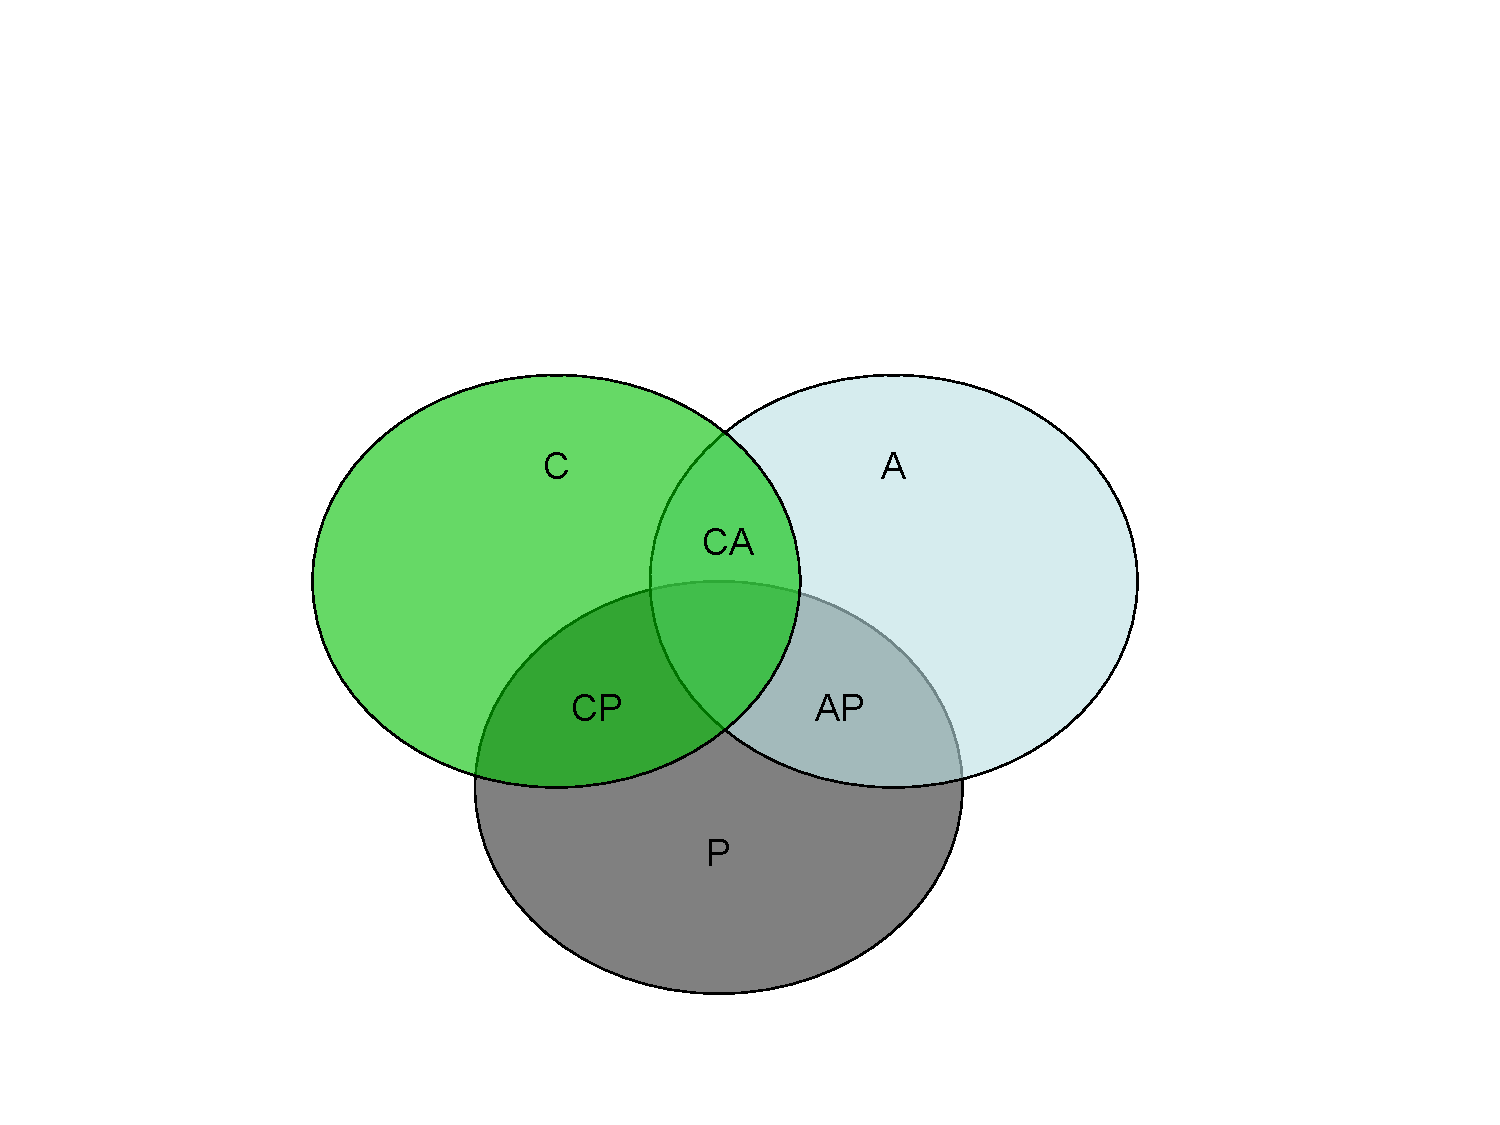
\includegraphics[scale=0.3]{./figures/cap_pick2}
\end{figure}
}

%%%%%%%%%%%%%%%%%%%%%%%%%%%%%%%%%%%%%%%%%%%%%%%%%%%%%%%%%%
\frame {\frametitle{Precautions: be careful with CA}
%%%%%%%%%%%%%%%%%%%%%%%%%%%%%%%%%%%%%%%%%%%%%%%%%%%%%%%%%%
\begin{itemize}
	\item {\bf Sacrificing P (partition tolerance)}

	\vspace{20pt}

	\item {\bf Negating:} A system functions properly even if the network is allowed to lose arbitrarily many messages sent from one node to another 

	\vspace{20pt}

	\item {\bf Yields:} A system {\color{red}does not} function properly even if the network is allowed to lose arbitrarily many messages sent from one node to another
	\begin{itemize}
		\item This implies sacrificing C or A, \textit{i.e.,} the system does not work
	\end{itemize}
\end{itemize}
}

%%%%%%%%%%%%%%%%%%%%%%%%%%%%%%%%%%%%%%%%%%%%%%%%%%%%%%%%%%
\frame {\frametitle{Precautions: be careful with CA}
%%%%%%%%%%%%%%%%%%%%%%%%%%%%%%%%%%%%%%%%%%%%%%%%%%%%%%%%%%
\begin{itemize}
	\item {\bf Negating P:} A system function properly if the network is {\color{red}not allowed} to lose arbitrarily many messages

	\vspace{20pt}

	\item {\bf However, in practice:} It is not possible to choose whether the network will lose messages! This either happens or not

	\vspace{20pt}

	\item {\bf One can argue that not ``arbitrarily'' many messages will be lost}
	\begin{itemize}
		\item But ``a lot'' of them might be (before the network repairs)
		\item In the meantime, either C or A is sacrificed
	\end{itemize}
\end{itemize}
}

%%%%%%%%%%%%%%%%%%%%%%%%%%%%%%%%%%%%%%%%%%%%%%%%%%%%%%%%%%
\frame {\frametitle{CAP in practice}
%%%%%%%%%%%%%%%%%%%%%%%%%%%%%%%%%%%%%%%%%%%%%%%%%%%%%%%%%%
\begin{itemize}
	\item {\bf In practical distributed systems:}
	\begin{itemize}
		\item Partitions may occur
		\item This is not under your control, as a system designer
	\end{itemize}

	\vspace{20pt}

	\item {\bf Designer's choice:}
	\begin{itemize}
		\item {\color{red}You choose} whether you want your system in C or A, when/if (temporary) partitions occur
	\end{itemize}

	\vspace{20pt}

	\item {\bf In summary:}
	\begin{itemize}
		\item CAP is a fundamental theorem stating the tradeoffs among different system properties
		\item {\color{red}Practical distributed systems are either in CP or AP}
		\item {\bf The choice (C vs. A) depends on your application logic}
	\end{itemize}
\end{itemize}
}

%%%%%%%%%%%%%%%%%%%%%%%%%%%%%%%%%%%%%%%%%%%%%%%%%%%%%%%%%%
\frame {\frametitle{CAP in theory}
%%%%%%%%%%%%%%%%%%%%%%%%%%%%%%%%%%%%%%%%%%%%%%%%%%%%%%%%%%
\begin{itemize}
	\item {\bf Historical notes:}
	\begin{itemize}
		\item First stated by Eric Brewer at the PODC 2000 keynote
		\item Formally proved by Gilbert and Lynch, 2002
	\end{itemize}

	\vspace{20pt}

	\item {\bf GL Theorems:}
	\begin{itemize}
		\item Asynchronous / partially synchronous network models
		\item Read/Write data objects
		\item Finer definitions of Availability and Consistency
	\end{itemize}

	\vspace{20pt}

	\item {\bf Further readings:}
	\begin{itemize}
		\item (Fischer, Lynch and Patterson) FLP impossibility result
		\item t-connected CAP
	\end{itemize}
\end{itemize}
}

%%%%%%%%%%%%%%%%%%%%%%%%%%%%%%%%%%%%%%%%%%%%%%%%%%%%%%%%%%
\frame {\frametitle{CAP: some illustrative choices}
%%%%%%%%%%%%%%%%%%%%%%%%%%%%%%%%%%%%%%%%%%%%%%%%%%%%%%%%%%
\begin{itemize}
	\item {\bf CP:}
	\begin{itemize}
		\item BigTable (Google), HBase, MongoDB, Redis, Memcachedb, ...
		\item (sometimes classified in CA) Paxos, Zookeeper, RDBMSs, ...
	\end{itemize}

	\vspace{40pt}

	\item {\bf AP:}
	\begin{itemize}
		\item Amazon Dynamo, CouchDB, Cassandra, SimpleDB, Riak, Voldmort (LinkedIn), ...
	\end{itemize}
\end{itemize}
}



%%%%%%%%%%%%%%%%%%%%%%%%%%%%%%%%%%%%%%%%%%%%%%%%%%%%%%%%%%
%%%%%%%%%%%%%%%%%%%%%%%%%%%%%%%%%%%%%%%%%%%%%%%%%%%%%%%%%%
\begin{frame}
 \begin{colorblock}{blue}{lightblue}{ }
  \begin{center}
    \Huge \textbf{\texttt{Amazon Dynamo}}
  \end{center}
  \end{colorblock}
\end{frame}
%%%%%%%%%%%%%%%%%%%%%%%%%%%%%%%%%%%%%%%%%%%%%%%%%%%%%%%%%%
%%%%%%%%%%%%%%%%%%%%%%%%%%%%%%%%%%%%%%%%%%%%%%%%%%%%%%%%%%
\section{Amazon Dynamo}
%%%%%%%%%%%%%%%%%%%%%%%%%%%%%%%%%%%%%%%%%%%%%%%%%%%%%%%%%%
\frame {\frametitle{Amazon Web Services}
%%%%%%%%%%%%%%%%%%%%%%%%%%%%%%%%%%%%%%%%%%%%%%%%%%%%%%%%%%
\begin{itemize}
	\item {\bf Amazon's cloud computing services}
	\begin{itemize}
		\item S3, EC2, RedShift, SimpleDB, Elastic MR, and many, many more
		\item Combined, they allow constructing Internet-scale applications
	\end{itemize}

	\item {\bf Infrastructure services requirements:}
	\begin{itemize}
		\item Security, scalability, availability, performance, cost-efficiency
		\item Serve millions of customers worldwide, continuously
	\end{itemize}
\end{itemize}
}

%%%%%%%%%%%%%%%%%%%%%%%%%%%%%%%%%%%%%%%%%%%%%%%%%%%%%%%%%%
\frame {\frametitle{Amazon Web Services}
%%%%%%%%%%%%%%%%%%%%%%%%%%%%%%%%%%%%%%%%%%%%%%%%%%%%%%%%%%
\begin{itemize}
	\item {\bf Important observations}
	\begin{itemize}
		\item No emphasis on consistency
		\item AWS is in AP, sacrificing consistency
	\end{itemize}

	\item {\bf AWS follows the BASE philosophy}
	\begin{itemize}
		\item BASE vs. ACID
		\item Basically Available
		\item Soft state
		\item Eventually consistent
	\end{itemize}
\end{itemize}
}

%%%%%%%%%%%%%%%%%%%%%%%%%%%%%%%%%%%%%%%%%%%%%%%%%%%%%%%%%%
\frame {\frametitle{Why favoring Availability over Consistency?}
%%%%%%%%%%%%%%%%%%%%%%%%%%%%%%%%%%%%%%%%%%%%%%%%%%%%%%%%%%
\begin{itemize}
	\item {\bf Even the shortest outage has significant financial consequences and impact customer trust}

	\item {\bf Clearly, consistency violations may as well have a big impact}
	\begin{itemize}
		\item But not in several Amazon's services
		\item {\color{red} Billing} is a separate story
	\end{itemize}
\end{itemize}
}

%%%%%%%%%%%%%%%%%%%%%%%%%%%%%%%%%%%%%%%%%%%%%%%%%%%%%%%%%%
\frame {\frametitle{Amazon Dynamo}
%%%%%%%%%%%%%%%%%%%%%%%%%%%%%%%%%%%%%%%%%%%%%%%%%%%%%%%%%%
\begin{itemize}
	\item {\bf Works behind the scenes in the context of AWS}
	\begin{itemize}
		\item Used to power client-facing services such as S3, and others
		\item Used to power internal Amazon services such as: shopping cart, customer session management, product catalog, recommendations, order fulfillment, sales rank, fraud detection, ...
	\end{itemize}

	\item {\bf What is Dynamo?}
	\begin{itemize}
		\item Highly available key-value storage system
		\item Favors availability over consistency under failures
	\end{itemize}
\end{itemize}
}

%%%%%%%%%%%%%%%%%%%%%%%%%%%%%%%%%%%%%%%%%%%%%%%%%%%%%%%%%%
\frame {\frametitle{What is a key-value store?}
%%%%%%%%%%%%%%%%%%%%%%%%%%%%%%%%%%%%%%%%%%%%%%%%%%%%%%%%%%
\begin{itemize}
	\item {\bf Think about Hash tables or dictionaries}
	\begin{itemize}
		\item Simple API: \texttt{\bf get(key)}, \texttt{\bf put(key, value)}
		\item Sometimes referred to read/write operations
	\end{itemize}

	\item {\bf Specifics of Dynamo API}
	\begin{itemize}
		\item Uses an additional argument to pass a ``context''
		\item Context holds critical metadata
		\item Typically stores {\color{red}small objects} (< 1 MB)
	\end{itemize}

	\item {\bf Specifics of services using Dynamo}
	\begin{itemize}
		\item Do not need transactions
		\item Often need only primary-key access to data
	\end{itemize}
\end{itemize}
}

%%%%%%%%%%%%%%%%%%%%%%%%%%%%%%%%%%%%%%%%%%%%%%%%%%%%%%%%%%
\frame {\frametitle{Amazon Dynamo: Features}
%%%%%%%%%%%%%%%%%%%%%%%%%%%%%%%%%%%%%%%%%%%%%%%%%%%%%%%%%%
\begin{itemize}
	\item {\bf Main characteristics}
	\begin{itemize}
		\item Low latency
		\item Scalable (hundreds of machines)
		\item Always-on available (especially for writes)
		\item Partition/Fault tolerance
		\item {\color{red}Eventually} consistent
	\end{itemize}

	\item {\bf How such features are obtained}
	\begin{itemize}
		\item General distributed systems toolbox
		\item We review some of them here
	\end{itemize}
\end{itemize}
}

%%%%%%%%%%%%%%%%%%%%%%%%%%%%%%%%%%%%%%%%%%%%%%%%%%%%%%%%%%
\frame {\frametitle{Amazon Dynamo: Key Techniques (1)}
%%%%%%%%%%%%%%%%%%%%%%%%%%%%%%%%%%%%%%%%%%%%%%%%%%%%%%%%%%
\begin{itemize}
	\item {\bf Consistent hashing} [Karger97]
	\begin{itemize}
		\item For data partitioning, replication and load balancing
	\end{itemize}

	\item {\bf Sloppy Quorums}
	\begin{itemize}
		\item Boosts availability in presence of failures
		\item May result in inconsistent versions of keys (data)
	\end{itemize}
\end{itemize}
}

%%%%%%%%%%%%%%%%%%%%%%%%%%%%%%%%%%%%%%%%%%%%%%%%%%%%%%%%%%
\frame {\frametitle{Amazon Dynamo: Key Techniques (2)}
%%%%%%%%%%%%%%%%%%%%%%%%%%%%%%%%%%%%%%%%%%%%%%%%%%%%%%%%%%
\begin{itemize}
	\item {\bf Vector clocks} [Fidge88/Mantern88]
	\begin{itemize}
		\item For tracking causal dependencies among different versions of the same key (data)
	\end{itemize}

	\item {\bf Gossip-based group membership}
	\begin{itemize}
		\item For maintaining information about alive nodes
	\end{itemize}

	\item {\bf Anti-entropy protocol based on Merkle trees}
	\begin{itemize}
		\item Background synchronization of divergent replicas
	\end{itemize}
\end{itemize}
}

%%%%%%%%%%%%%%%%%%%%%%%%%%%%%%%%%%%%%%%%%%%%%%%%%%%%%%%%%%
\frame {\frametitle{Amazon Dynamo: Design Decisions}
%%%%%%%%%%%%%%%%%%%%%%%%%%%%%%%%%%%%%%%%%%%%%%%%%%%%%%%%%%
\begin{itemize}
	\item {\bf Always writable data store}
	\begin{itemize}
		\item E.g., think shopping cart service
	\end{itemize}

	\item {\bf How to handle data changes?}
	\begin{itemize}
		\item Replication, required for fault/disaster tolerance
		\item Allow multiple versions of data
		\item Reconcile and resolve conflicts {\color{red}during reads}
	\end{itemize}

	\item {\bf How to reconcile data?}
	\begin{itemize}
		\item Application-side: depending on business logic
		\item Dynamo: deterministic, e.g., ``last-write'' wins
	\end{itemize}
\end{itemize}
}




\subsection{Dynamo Architecture}
%%%%%%%%%%%%%%%%%%%%%%%%%%%%%%%%%%%%%%%%%%%%%%%%%%%%%%%%%%
%%%%%%%%%%%%%%%%%%%%%%%%%%%%%%%%%%%%%%%%%%%%%%%%%%%%%%%%%%
\begin{frame}
 \begin{colorblock}{blue}{lightblue}{ }
  \begin{center}
    \textbf{\texttt{Amazon Dynamo: Architecture}}
  \end{center}
  \end{colorblock}
\end{frame}
%%%%%%%%%%%%%%%%%%%%%%%%%%%%%%%%%%%%%%%%%%%%%%%%%%%%%%%%%%
%%%%%%%%%%%%%%%%%%%%%%%%%%%%%%%%%%%%%%%%%%%%%%%%%%%%%%%%%%

%%%%%%%%%%%%%%%%%%%%%%%%%%%%%%%%%%%%%%%%%%%%%%%%%%%%%%%%%%
\frame {\frametitle{Amazon Dynamo Architecture}
%%%%%%%%%%%%%%%%%%%%%%%%%%%%%%%%%%%%%%%%%%%%%%%%%%%%%%%%%%
\begin{itemize}
	\item {\bf Scalable and robust components for:}
	\begin{itemize}
		\item {\bf Load balancing and data partitioning}
		\item {\bf Membership, fault detection}
		\item Failure recovery
		\item {\bf Replica synchronization}
		\item Overload Handling
		\item State transfer
		\item Concurrency management
		\item Scheduling
		\item Request marshalling and routing
		\item System monitoring
		\item Configuration management
	\end{itemize}

\end{itemize}
}

%%%%%%%%%%%%%%%%%%%%%%%%%%%%%%%%%%%%%%%%%%%%%%%%%%%%%%%%%%
\frame {\frametitle{Amazon Dynamo: Data Partitioning}
%%%%%%%%%%%%%%%%%%%%%%%%%%%%%%%%%%%%%%%%%%%%%%%%%%%%%%%%%%
\begin{itemize}
	\item {\bf Data partitioning}
	\begin{itemize}
		\item Dynamic partitioning of {\color{red}keys} over a set of storage {\color{red}nodes}
		\item Technique used for DHTs, e.g., Chord
	\end{itemize}

	\item {\bf Consistent Hashing}
	\begin{itemize}
		\item Hashes of keys give key $m$-bit identifiers
		\item Hashes of nodes give $m$-bit identifiers
		\item Identifiers are ordered in an identifier circle
	\end{itemize}

	\item {\bf Key assignment to storage nodes}
	\begin{itemize}
		\item A key is assigned to the closest {\color{red}successor node} ID
		\item Key $k$ is assigned to the first node whose ID $\geq k$
		\item If such node does not exist, navigate the circle and find node with the smallest ID
	\end{itemize}
\end{itemize}
}

%%%%%%%%%%%%%%%%%%%%%%%%%%%%%%%%%%%%%%%%%%%%%%%%%%%%%%%%%%
\frame {\frametitle{Consistent Hashing Example}
%%%%%%%%%%%%%%%%%%%%%%%%%%%%%%%%%%%%%%%%%%%%%%%%%%%%%%%%%%
\begin{itemize}
	\item Assume: $m=3$ bit, 3 storage nodes (0,2,3), 4 keys (1,3,5,6)
\end{itemize}
\begin{figure}[h]
	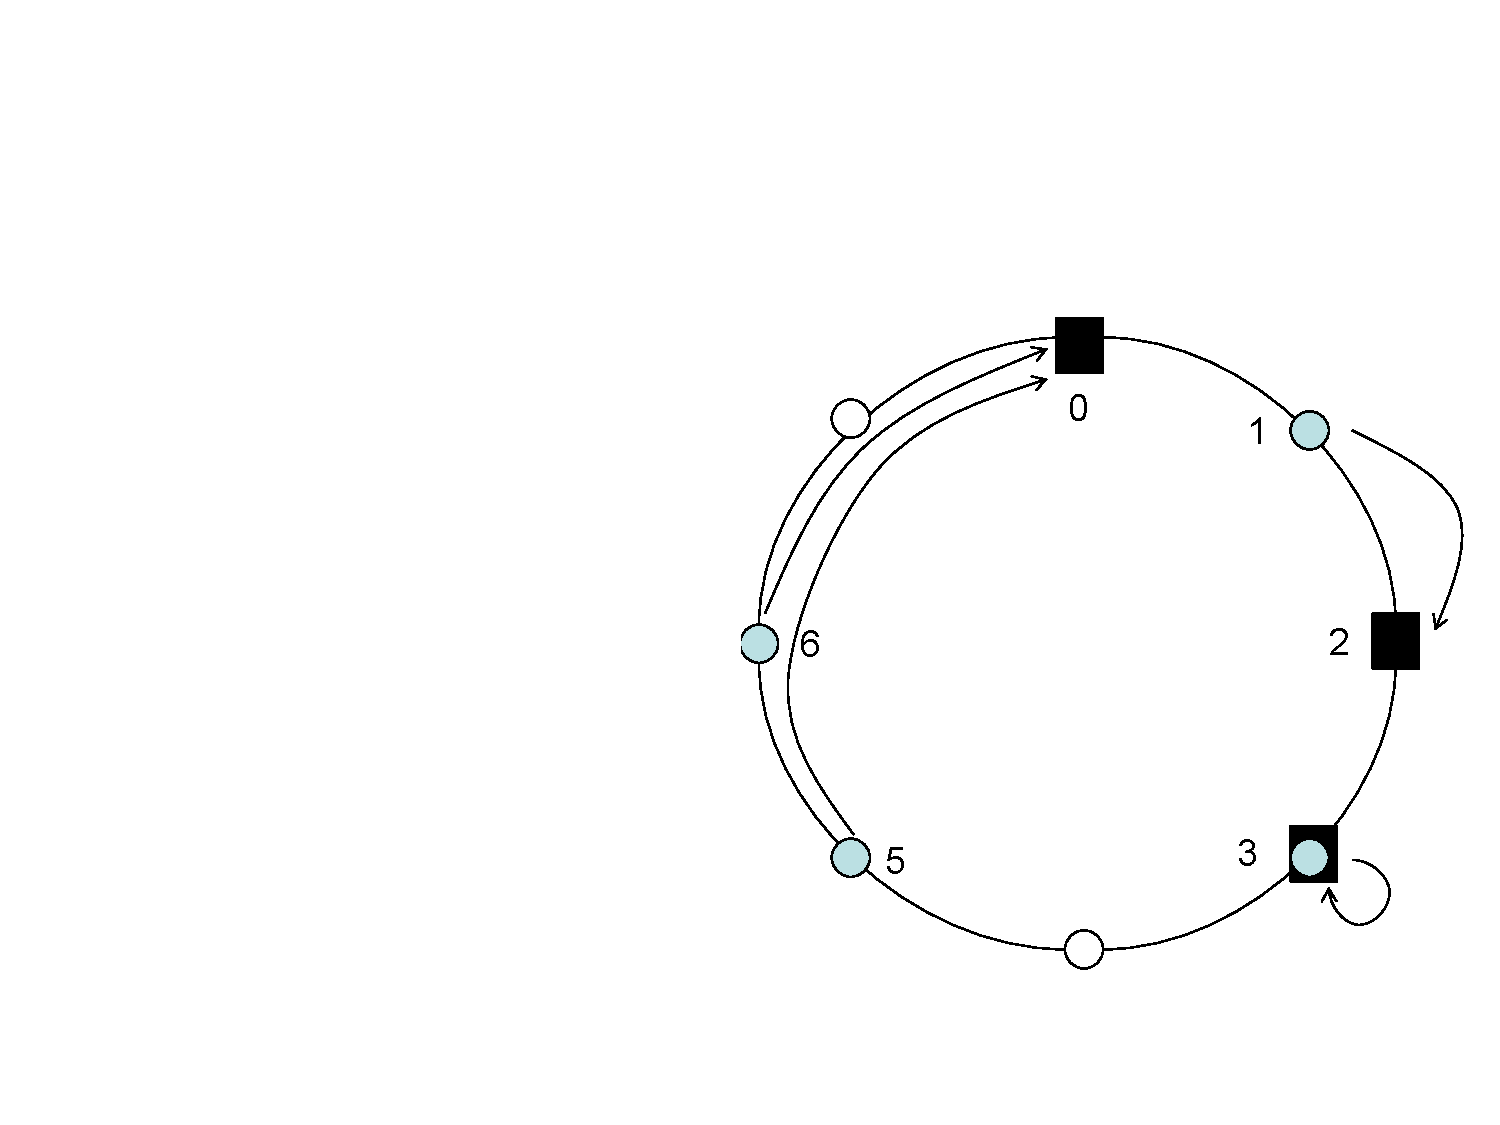
\includegraphics[scale=0.3]{./figures/consistent_hashing_example}
\end{figure}
}

%%%%%%%%%%%%%%%%%%%%%%%%%%%%%%%%%%%%%%%%%%%%%%%%%%%%%%%%%%
\frame {\frametitle{Consistent Hashing: Key Properties (1)}
%%%%%%%%%%%%%%%%%%%%%%%%%%%%%%%%%%%%%%%%%%%%%%%%%%%%%%%%%%
\begin{itemize}
	\item {\bf Dynamic membership management}
	\begin{itemize}
		\item Storage nodes can come and go
		\item Allows incremental scalability
	\end{itemize}

	\item {\bf Storage node arrival/departures}
	\begin{itemize}
		\item \texttt{$n$ Joins}: all keys previously assigned to node $n$'s successor are now assigned to $n$
		\item \texttt{$n$ Leaves}: all keys currently assigned to node $n$ are assigned to its successor
	\end{itemize}
\end{itemize}
}

%%%%%%%%%%%%%%%%%%%%%%%%%%%%%%%%%%%%%%%%%%%%%%%%%%%%%%%%%%
\frame {\frametitle{Consistent Hashing: Key Properties (2)}
%%%%%%%%%%%%%%%%%%%%%%%%%%%%%%%%%%%%%%%%%%%%%%%%%%%%%%%%%%
\begin{itemize}
	\item {\bf Load balancing} [Karger97]
	\begin{itemize}
		\item Each node is responsible for at most $(1+ \epsilon)K/N$ keys
		\item When a new node joins, only $O(K/n)$ keys must be moved (optimal)
	\end{itemize}

	\item {\bf Virtual Nodes}
	\begin{itemize}
		\item Each physical storage node mapped multiple times to the circle
		\item[$\to$] Improves load balancing
		\item[$\to$] Allows heterogeneous storage nodes
	\end{itemize}
\end{itemize}
}

%%%%%%%%%%%%%%%%%%%%%%%%%%%%%%%%%%%%%%%%%%%%%%%%%%%%%%%%%%
\frame {\frametitle{Amazon Dynamo: Data Replication}
%%%%%%%%%%%%%%%%%%%%%%%%%%%%%%%%%%%%%%%%%%%%%%%%%%%%%%%%%%
\begin{itemize}
	\item {\bf Goal: achieve high availability and durability}
	\begin{itemize}
		\item Each data item (key) replicated at $N$ nodes
		\item Virtual nodes: same physical node skipped
		\item $N$ is a configurable parameter per Dynamo instance
	\end{itemize}

	\item {\bf Example:}
	\begin{itemize}
		\item Assume $N=3$
		\item For key $k$, $B$ is the ``coordinator'' node
		\item $B$ replicates $k$ to $N-1$ other successor nodes (C and D)
		\item[$\to$] $B, C, D$ are a {\bf preference list} for $k$
	\end{itemize}
\end{itemize}

\begin{figure}[h]
	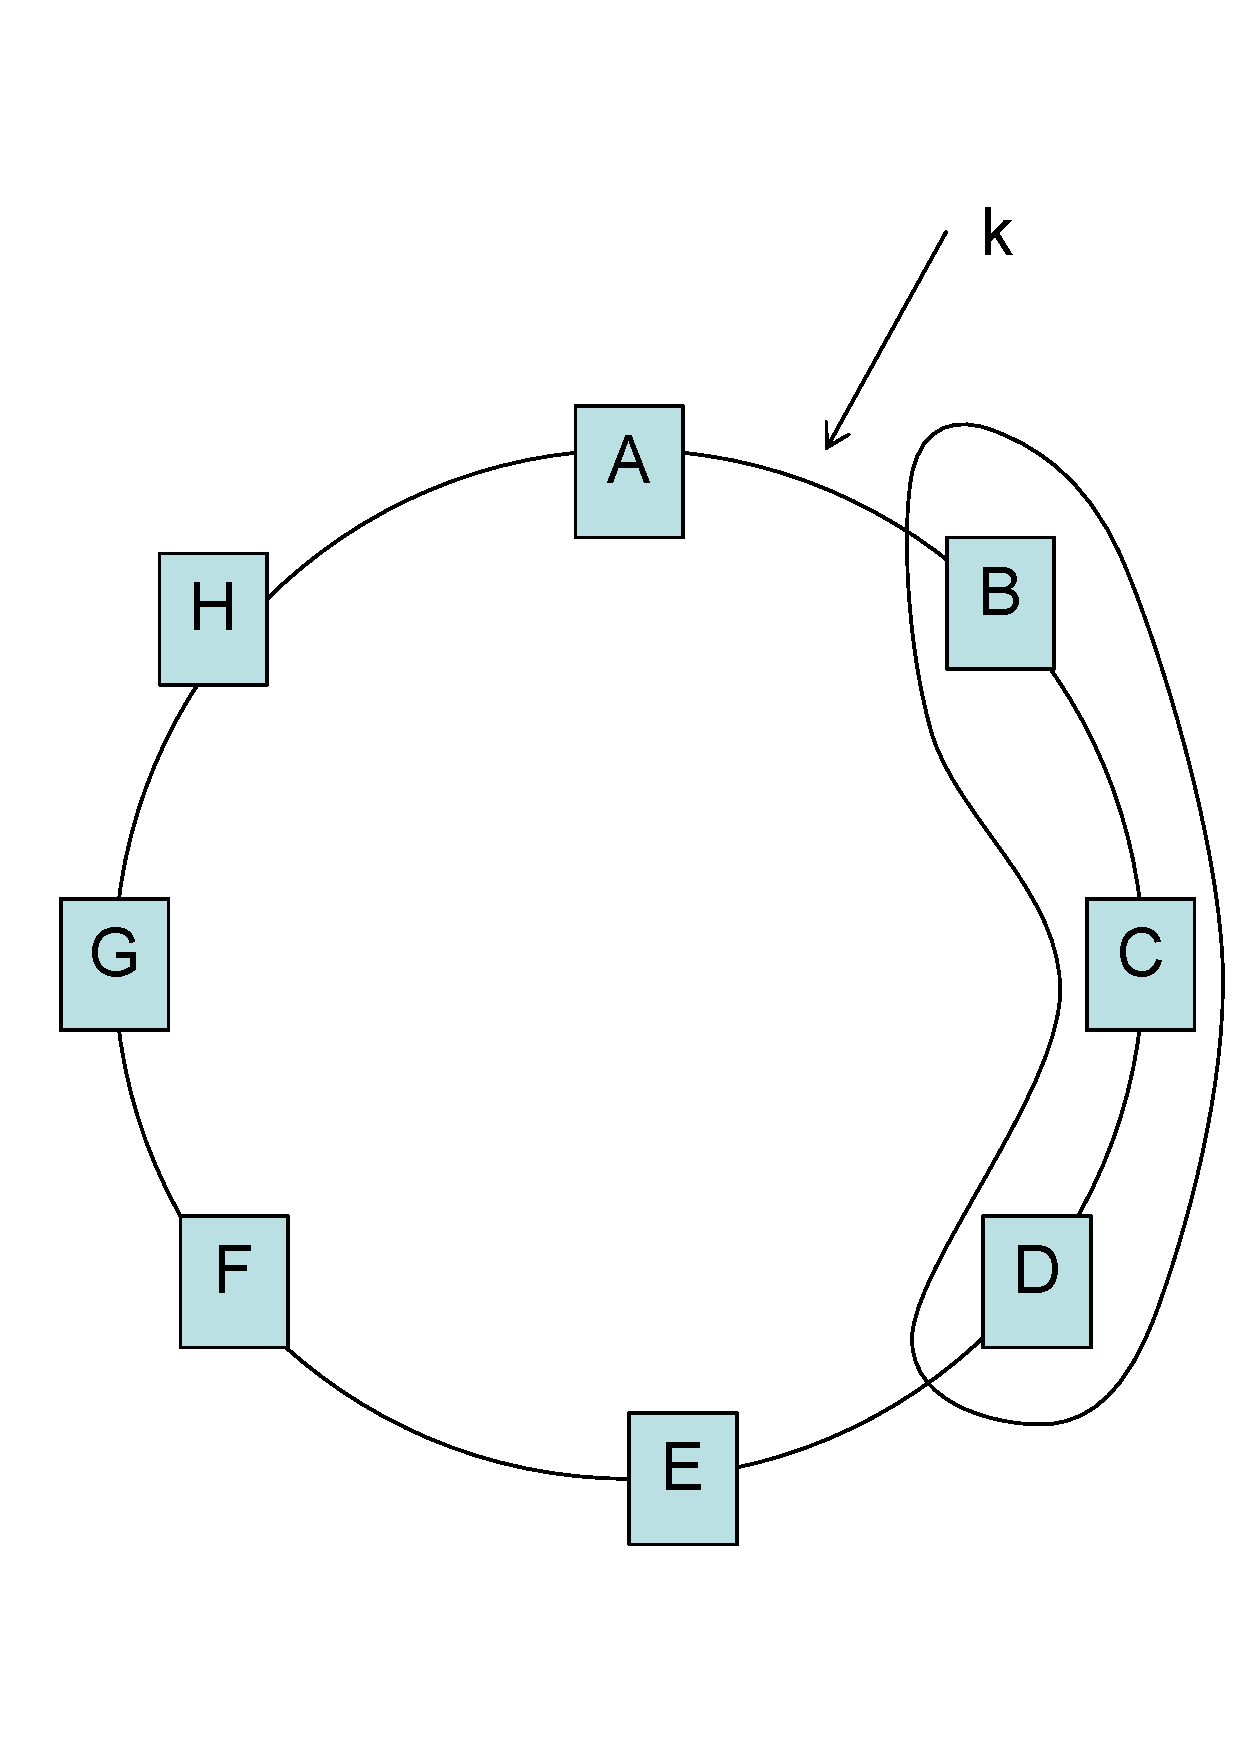
\includegraphics[scale=0.3]{./figures/dynamo_replication_example}
\end{figure}

}

%%%%%%%%%%%%%%%%%%%%%%%%%%%%%%%%%%%%%%%%%%%%%%%%%%%%%%%%%%
\frame {\frametitle{Amazon Dynamo: Data Versioning (1)}
%%%%%%%%%%%%%%%%%%%%%%%%%%%%%%%%%%%%%%%%%%%%%%%%%%%%%%%%%%
\begin{itemize}
	\item {\bf Data replication performed after an ACK is sent to a client \texttt{put} request}
	\begin{itemize}
		\item {\color{red}Asynchronous replication}
		\item May result in inconsistencies under partitions
		\item[$\to$] Read does not return the last value
	\end{itemize}

	\item {\bf Operations should not be lost!}
	\begin{itemize}
		\item ``Add to cart'' should not be rejected but also not forgotten
		\item If it is performed when the latest version is not available, then it is performed on a stale version of the data
		\item[$\to$] We may have different version of a key/value pair
	\end{itemize}
\end{itemize}
}

%%%%%%%%%%%%%%%%%%%%%%%%%%%%%%%%%%%%%%%%%%%%%%%%%%%%%%%%%%
\frame {\frametitle{Amazon Dynamo: Data Versioning (2)}
%%%%%%%%%%%%%%%%%%%%%%%%%%%%%%%%%%%%%%%%%%%%%%%%%%%%%%%%%%
\begin{itemize}
	\item {\bf Precautions}
	\begin{itemize}
		\item Once a partition heals, versions are merged
		\item New versions subsume previous ones
		\item Applications {\color{red}must be designed} with data versionin in mind
	\end{itemize}

	\item {\bf Key technique for versioning}
	\begin{itemize}
		\item Vector clocks
		\item Capture causality between different versions of an object
	\end{itemize}
\end{itemize}
}

%%%%%%%%%%%%%%%%%%%%%%%%%%%%%%%%%%%%%%%%%%%%%%%%%%%%%%%%%%
\frame {\frametitle{Vector Clocks (in Dynamo) (1)}
%%%%%%%%%%%%%%%%%%%%%%%%%%%%%%%%%%%%%%%%%%%%%%%%%%%%%%%%%%
\begin{itemize}
	\item {\bf In theory:}
	\begin{itemize}
		\item Each \texttt{write} to a key $k$ associated to a vector clock $VC(k)$
		\item $VC(k)$ is an array (map) of integers
		\item In theory, one entry $VC(k)[i]$ for each storage node $i$
		\item When node $i$ handles a write for key $k$ it increments $VC(k)[i]$
	\end{itemize}

	\item {\bf In practice:}
	\begin{itemize}
		\item $VC(k)$ will not have many entries $\to$ only node from the preference list should have entries
		\item Dynamo truncates entries if more than a threshold
	\end{itemize}
\end{itemize}
}

%%%%%%%%%%%%%%%%%%%%%%%%%%%%%%%%%%%%%%%%%%%%%%%%%%%%%%%%%%
\frame {\frametitle{Vector Clocks (in Dynamo) (2)}
%%%%%%%%%%%%%%%%%%%%%%%%%%%%%%%%%%%%%%%%%%%%%%%%%%%%%%%%%%
\begin{figure}[h]
	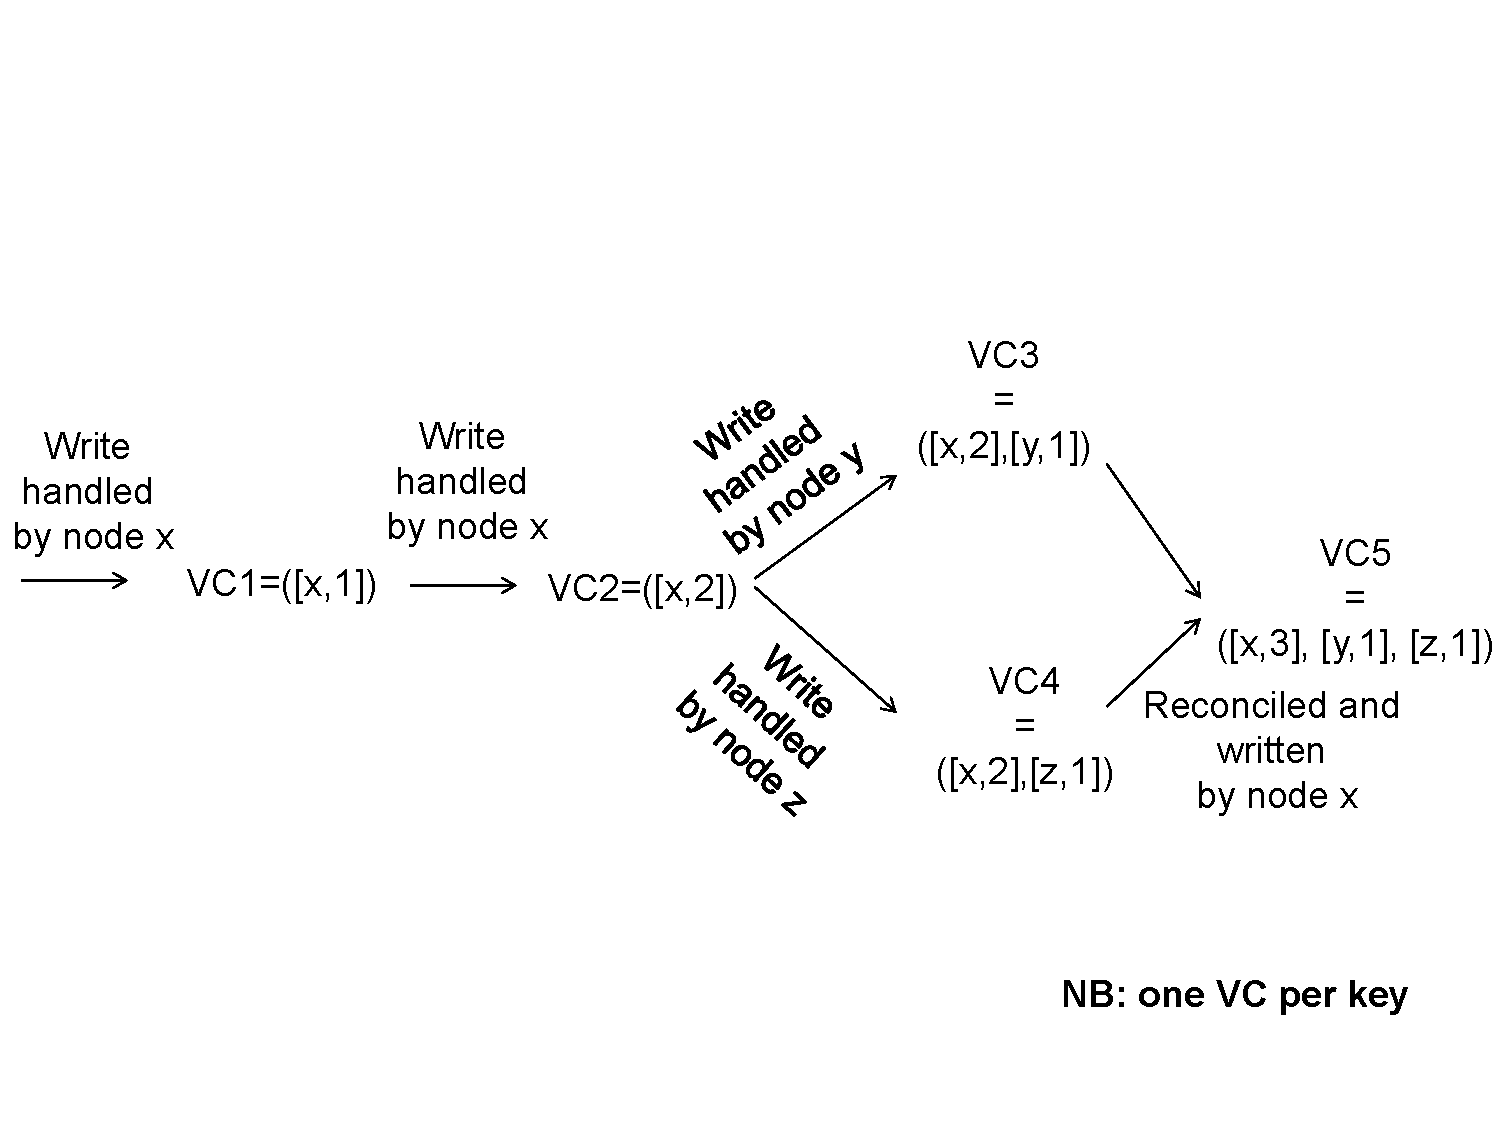
\includegraphics[scale=0.5]{./figures/dynamo_vc_example}
\end{figure}

}

%%%%%%%%%%%%%%%%%%%%%%%%%%%%%%%%%%%%%%%%%%%%%%%%%%%%%%%%%%
\frame {\frametitle{Anatomy of \texttt{put} and \texttt{get} operations}
%%%%%%%%%%%%%%%%%%%%%%%%%%%%%%%%%%%%%%%%%%%%%%%%%%%%%%%%%%
\begin{itemize}
	\item {\bf Storage nodes can receive requests for {\color{red}any} key}
	\begin{itemize}
		\item Generic load balancer may chose a random node, not necessarily the coordinator
		\item Application may directly contact the coordinator in a preference list
	\end{itemize}

	\item {\bf Request routing}
	\begin{itemize}
		\item Node serves request only if in preference list
		\item Otherwise, routes the request to the first node in preference list
		\item 0-hop DHT routing: all nodes know all other nodes
		\item[$\to$] Not the most scalable, but excellent for low-latency
	\end{itemize}

	\item {\bf Extended preference list}
	\begin{itemize}
		\item Accounts for node failures
	\end{itemize}
\end{itemize}
}

%%%%%%%%%%%%%%%%%%%%%%%%%%%%%%%%%%%%%%%%%%%%%%%%%%%%%%%%%%
\frame {\frametitle{Amazon Dynamo: Quorums}
%%%%%%%%%%%%%%%%%%%%%%%%%%%%%%%%%%%%%%%%%%%%%%%%%%%%%%%%%%
\begin{itemize}
	\item {\bf Two important parameters}
	\begin{itemize}
		\item R: number of nodes involved in a get
		\item W: number of nodes involved in a put
		\item Quorum system: $R+W > N$, where $N$ is the number of replicas
	\end{itemize}

	\item {\bf Handling put (by coordinator)}
	\begin{itemize}
		\item Generate new VC, write new version locally
		\item Send value, VC, to $N$ nodes from preference list
		\item Wait for $W-1$ acknowledgments
	\end{itemize}

	\item {\bf Handling get (by coordinator)}
	\begin{itemize}
		\item Send get to $N$ selected nodes from preference list
		\item Wait for $R$ responses
		\item Select highest versions using VC, reconcile/merge different versions
		\item Writeback reconciled version
	\end{itemize}
\end{itemize}
}

%%%%%%%%%%%%%%%%%%%%%%%%%%%%%%%%%%%%%%%%%%%%%%%%%%%%%%%%%%
\frame {\frametitle{Choosing $R, W$}
%%%%%%%%%%%%%%%%%%%%%%%%%%%%%%%%%%%%%%%%%%%%%%%%%%%%%%%%%%
\begin{itemize}
	\item {\bf $R,W$ smaller than $N$}
	\begin{itemize}
		\item To decrease latency
		\item Slowest replica dictates query latency
	\end{itemize}

	\item {\bf $W=1$}
	\begin{itemize}
		\item Always available for writes
		\item Yields $R=N$ $\to$ reads pay the penalty
	\end{itemize}

	\item {\bf Typical values in Dynamo}
	\begin{itemize}
		\item $W,R,N = 2,2,3$
	\end{itemize}
\end{itemize}
}

%%%%%%%%%%%%%%%%%%%%%%%%%%%%%%%%%%%%%%%%%%%%%%%%%%%%%%%%%%
\frame {\frametitle{Handling Failures}
%%%%%%%%%%%%%%%%%%%%%%%%%%%%%%%%%%%%%%%%%%%%%%%%%%%%%%%%%%
\begin{itemize}
	\item {\bf $N$ selected nodes are the first $N$ healthy nodes}
	\begin{itemize}
		\item Might change from request to request
		\item Hence the term ``sloppy'' quorums
	\end{itemize}

	\item {\bf Sloppy vs. strict quorums}
	\begin{itemize}
		\item Allow availability under a much wider range of partitions
		\item Sacrifice consistency
	\end{itemize}

	\item {\bf Data-center wide failures}
	\begin{itemize}
		\item Power outages, cooling failures, network failures, ...
		\item Preference lists account for this
	\end{itemize}
\end{itemize}
}

%%%%%%%%%%%%%%%%%%%%%%%%%%%%%%%%%%%%%%%%%%%%%%%%%%%%%%%%%%
\frame {\frametitle{Handling Temporary Failures}
%%%%%%%%%%%%%%%%%%%%%%%%%%%%%%%%%%%%%%%%%%%%%%%%%%%%%%%%%%
\begin{itemize}
	\item {\bf Hinted Handoff}
	\begin{itemize}
		\item If a replica in the preference list is down, then a new replica is created on a new node
		\item Coordinator selects a new replica node, but hints that the role is temporary
		\item When the new replica learns about failure recovery, it handles data to the node in the preference list
	\end{itemize}
\end{itemize}
}

%%%%%%%%%%%%%%%%%%%%%%%%%%%%%%%%%%%%%%%%%%%%%%%%%%%%%%%%%%
\frame {\frametitle{Amazon Dynamo: Anti-Entropy Synchronization}
%%%%%%%%%%%%%%%%%%%%%%%%%%%%%%%%%%%%%%%%%%%%%%%%%%%%%%%%%%
\begin{itemize}
	\item {\bf Uses Merkle Trees}
	\begin{itemize}
		\item A tree in which every non-leaf node is labelled with the hash of the labels of its children nodes
	\end{itemize}

	\item {\bf Storage nodes}
	\begin{itemize}
		\item Keep a Merkle tree for each of its key ranges (virtual nodes)
		\item Compare root of the tree with replicas
		\item If equal, replicas are in sync
		\item Otherwise, traverse the tree and synchronize keys that differ
	\end{itemize}
\end{itemize}
}

%%%%%%%%%%%%%%%%%%%%%%%%%%%%%%%%%%%%%%%%%%%%%%%%%%%%%%%%%%
\frame {\frametitle{Amazon Dynamo: Membership Management}
%%%%%%%%%%%%%%%%%%%%%%%%%%%%%%%%%%%%%%%%%%%%%%%%%%%%%%%%%%
\begin{itemize}
	\item {\bf Membership management initiated by administrator}

	\item {\bf Gossip protocol to propagate membership changes}
	\begin{itemize}
		\item Nodes contact a random node every second
		\item 2 nodes reconcile membership information
		\item Gossiping also used to handle metadata
	\end{itemize}
\end{itemize}
}

%%%%%%%%%%%%%%%%%%%%%%%%%%%%%%%%%%%%%%%%%%%%%%%%%%%%%%%%%%
\frame {\frametitle{Failure Detection}
%%%%%%%%%%%%%%%%%%%%%%%%%%%%%%%%%%%%%%%%%%%%%%%%%%%%%%%%%%
\begin{itemize}
	\item {\bf Unreliable failure detection}
	\begin{itemize}
		\item Detection is triggered by read/write requests
		\item Called ``in-band'' failure detection
		\item[$\to$] No dedicated component
	\end{itemize}

	\item {\bf Example:}
	\begin{itemize}
		\item With steady load on node A
		\item Node A periodically checks the status of nodes in the extended preference list
		\item {\color{red} Does not make the distinction between faults and partitions}
	\end{itemize}
\end{itemize}
}

%%%%%%%%%%%%%%%%%%%%%%%%%%%%%%%%%%%%%%%%%%%%%%%%%%%%%%%%%%
\frame {\frametitle{Amazon Dynamo: Summary}
%%%%%%%%%%%%%%%%%%%%%%%%%%%%%%%%%%%%%%%%%%%%%%%%%%%%%%%%%%
\begin{itemize}
	\item {\bf Eventually consistent, highly available key value store}
	\begin{itemize}
		\item In the CAP space, it is in AP
	\end{itemize}

	\item {\bf Focuses on low-latency}
	\begin{itemize}
		\item Writes are super fast
		\item Reconciliation in reads
	\end{itemize}

	\item {\bf Built atop of fundamental techniques in distributed systems}
	\begin{itemize}
		\item Consistent hashing
		\item Sloppy quorum-based replication
		\item Merkle-tree based synchronization
		\item Vector clocks, and gossip membership management
	\end{itemize}
\end{itemize}
}



%%%%%%%%%%%%%%%%%%%%%%%%%%%%%%%%%%%%%%%%%%%%%%%%%%%%%%%%%%
%%%%%%%%%%%%%%%%%%%%%%%%%%%%%%%%%%%%%%%%%%%%%%%%%%%%%%%%%%
\begin{frame}
 \begin{colorblock}{blue}{lightblue}{ }
  \begin{center}
    \Huge \textbf{\texttt{HBASE}}
  \end{center}
  \end{colorblock}
\end{frame}
%%%%%%%%%%%%%%%%%%%%%%%%%%%%%%%%%%%%%%%%%%%%%%%%%%%%%%%%%%
%%%%%%%%%%%%%%%%%%%%%%%%%%%%%%%%%%%%%%%%%%%%%%%%%%%%%%%%%%
\section{HBase}
\subsection{Introduction}
%%%%%%%%%%%%%%%%%%%%%%%%%%%%%%%%%%%%%%%%%%%%%%%%%%%%%%%%%%
\begin{frame}
  \begin{beamerboxesrounded}{}
	\begin{center}

\vspace{20pt}

		Introduction

\vspace{20pt}

	\end{center}    
  \end{beamerboxesrounded}
\end{frame}


%%%%%%%%%%%%%%%%%%%%%%%%%%%%%%%%%%%%%%%%%%%%%%%%%%%%%%%%%%
\subsection{RDBMS}
%%%%%%%%%%%%%%%%%%%%%%%%%%%%%%%%%%%%%%%%%%%%%%%%%%%%%%%%%%
\frame {\frametitle{Why yet another storage architecture?}
  \begin{itemize}
  \item \textbf{Relational Databse Management Systems (RDBMS)}:
    \begin{itemize}
    \item Around since 1970s
    \item Countless examples in which they actually do make sense
    \end{itemize}

\vspace{20pt}

  \item \textbf{The dawn of Big Data}:
    \begin{itemize}
    \item Previously: ignore data sources because no cost-effective
      way to store everything
      \begin{itemize}
      \item One option was to prune, by retaining only data for the
        last $N$ days
      \end{itemize}
    \item Today: store everything!
      \begin{itemize}
      \item Pruning fails in providing a base to build useful
        mathematical models
      \end{itemize}
    \end{itemize}
 \end{itemize}
}

\frame {\frametitle{Batch processing}
  \begin{itemize}
  \item \textbf{Hadoop and MapReduce}:
    \begin{itemize}
    \item Excels at storing (semi- and/or un-) structured data
    \item Data interpretation takes place at analysis-time
    \item Flexibility in data classification
    \end{itemize}

    \vspace{20pt}
    
  \item \textbf{Batch processing: A complement to RDBMS}
    \begin{itemize}
    \item Scalable sink for data, processing launched when time is
      right
    \item Optimized for large file storage
    \item Optimized for ``streaming'' access
    \end{itemize}

    \vspace{20pt}
    
  \item \textbf{Random Access}:
    \begin{itemize}
    \item Users need to ``interact'' with data, especially that
      ``crunched'' after a MapReduce job
    \item This is historically where RDBMS excel: random access for
      structured data
    \end{itemize}
    
  \end{itemize}
}

%%%%%%%%%%%%%%%%%%%%%%%%%%%%%%%%%%%%%%%%%%%%%%%%%%%%%%%%%%
\subsection{Column-Oriented DB}
%%%%%%%%%%%%%%%%%%%%%%%%%%%%%%%%%%%%%%%%%%%%%%%%%%%%%%%%%%
\frame {\frametitle{Column-Oriented Databases}
  \begin{itemize}
  \item \textbf{Data layout}:
    \begin{itemize}
    \item Save their data grouped by columns
    \item Subsequent column values are stored contiguously on disk
    \item This is substantially different from  traditional RDBMS,
      which save and store data by row
    \end{itemize}

    \vspace{20pt}
    
  \item \textbf{Specialized databases for specific workloads}:
    \begin{itemize}
    \item Reduced I/O
    \item Better suited for compression $\to$ Efficient use of bandwidth
      \begin{itemize}
      \item Indeed, column values are often very similar and differ
        little row-by-row
      \end{itemize}
    \item Real-time access to data
    \end{itemize}

    \vspace{20pt}
    
  \item \textbf{Important NOTE}:
    \begin{itemize}
    \item HBase is not a column-oriented DB in the typical term
    \item HBase uses an on-disk column storage format
    \item Provides key-based access to specific cell of data, or a
      sequential range of cells
    \end{itemize}

  \end{itemize}
}

\frame {\frametitle{Column-Oriented and Row-Oriented storage layouts}
  \begin{figure}[h]
    \centering
    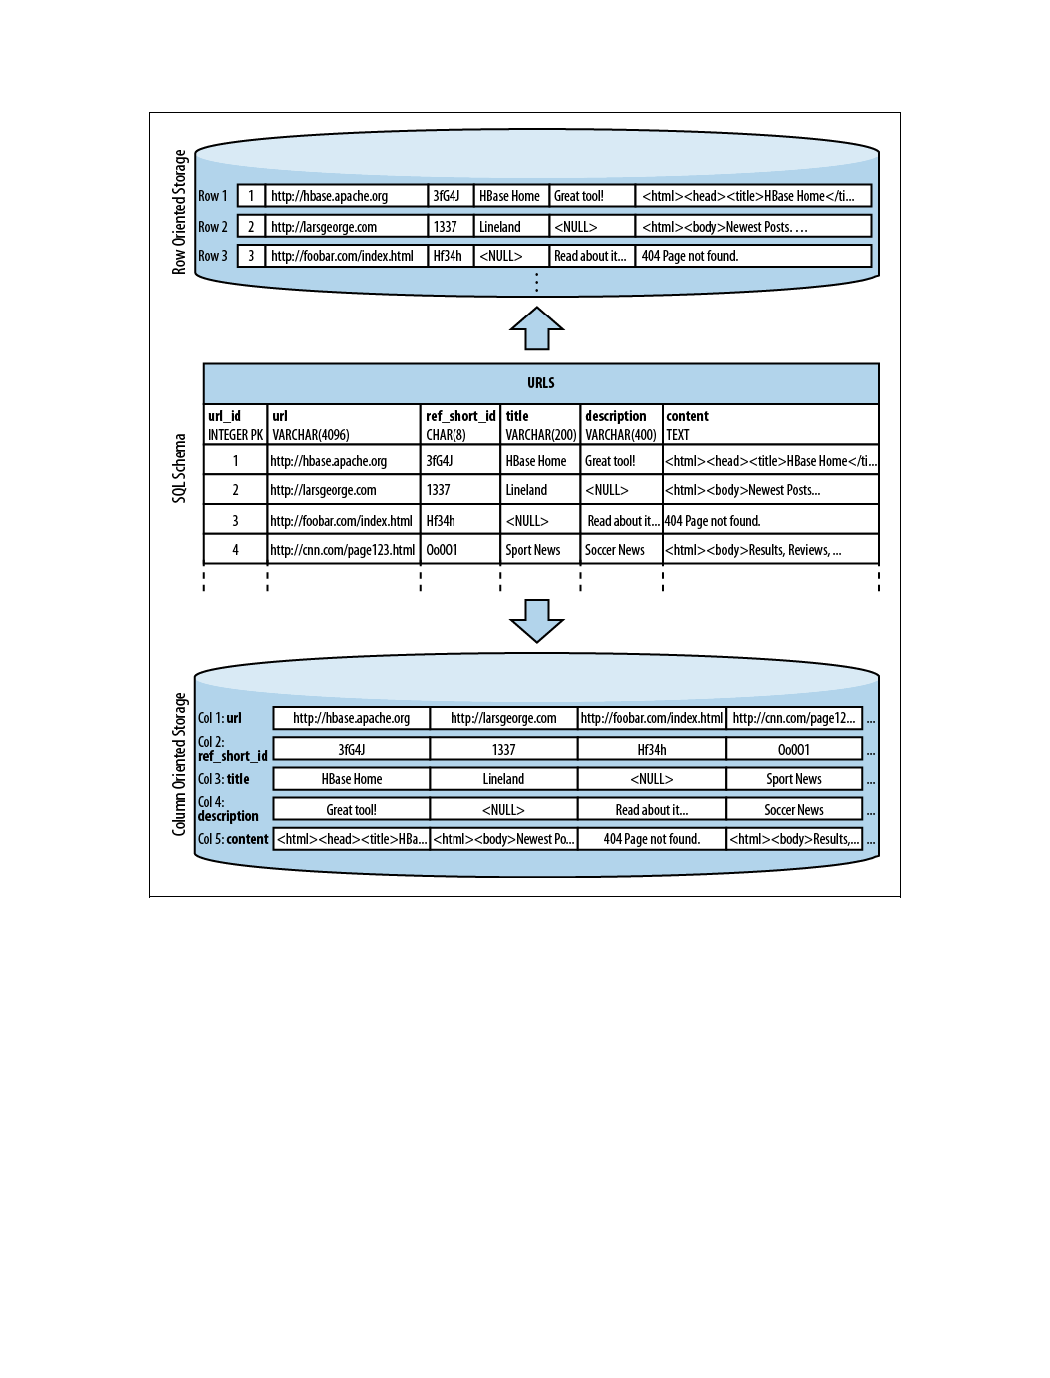
\includegraphics[scale=0.5]{./figures/storage-layout}
    \caption{Example of Storage Layouts}
    \label{fig:storage-layout}
  \end{figure}
}

%%%%%%%%%%%%%%%%%%%%%%%%%%%%%%%%%%%%%%%%%%%%%%%%%%%%%%%%%%
\subsection{The problem with RDBMS}
%%%%%%%%%%%%%%%%%%%%%%%%%%%%%%%%%%%%%%%%%%%%%%%%%%%%%%%%%%
\frame {\frametitle{The Problem with RDBMS}
  \begin{itemize}
  \item \textbf{RDBMS are still relevant}
    \begin{itemize}
    \item Persistence layer for frontend application
    \item Store relational data
    \item Works well for a limited number of records
    \end{itemize}

    \vspace{20pt}

  \item \textbf{Example: Hush}
    \begin{itemize}
    \item Used throughout this course
    \item URL shortener service
    \end{itemize}

    \vspace{20pt}

  \item \textbf{Let's see the ``scalability story'' of such a service}
    \begin{itemize}
    \item Assumption: service must run with a reasonable budget
    \end{itemize}

  \end{itemize}
}

\frame {\frametitle{The Problem with RDBMS}
  \begin{itemize}
  \item \textbf{Few thousands users: use a LAMP stack}
    \begin{itemize}
    \item \textit{Normalize data}
    \item Use foreign keys
    \item Use Indexes
    \end{itemize}

    \begin{figure}[h]
      \centering
      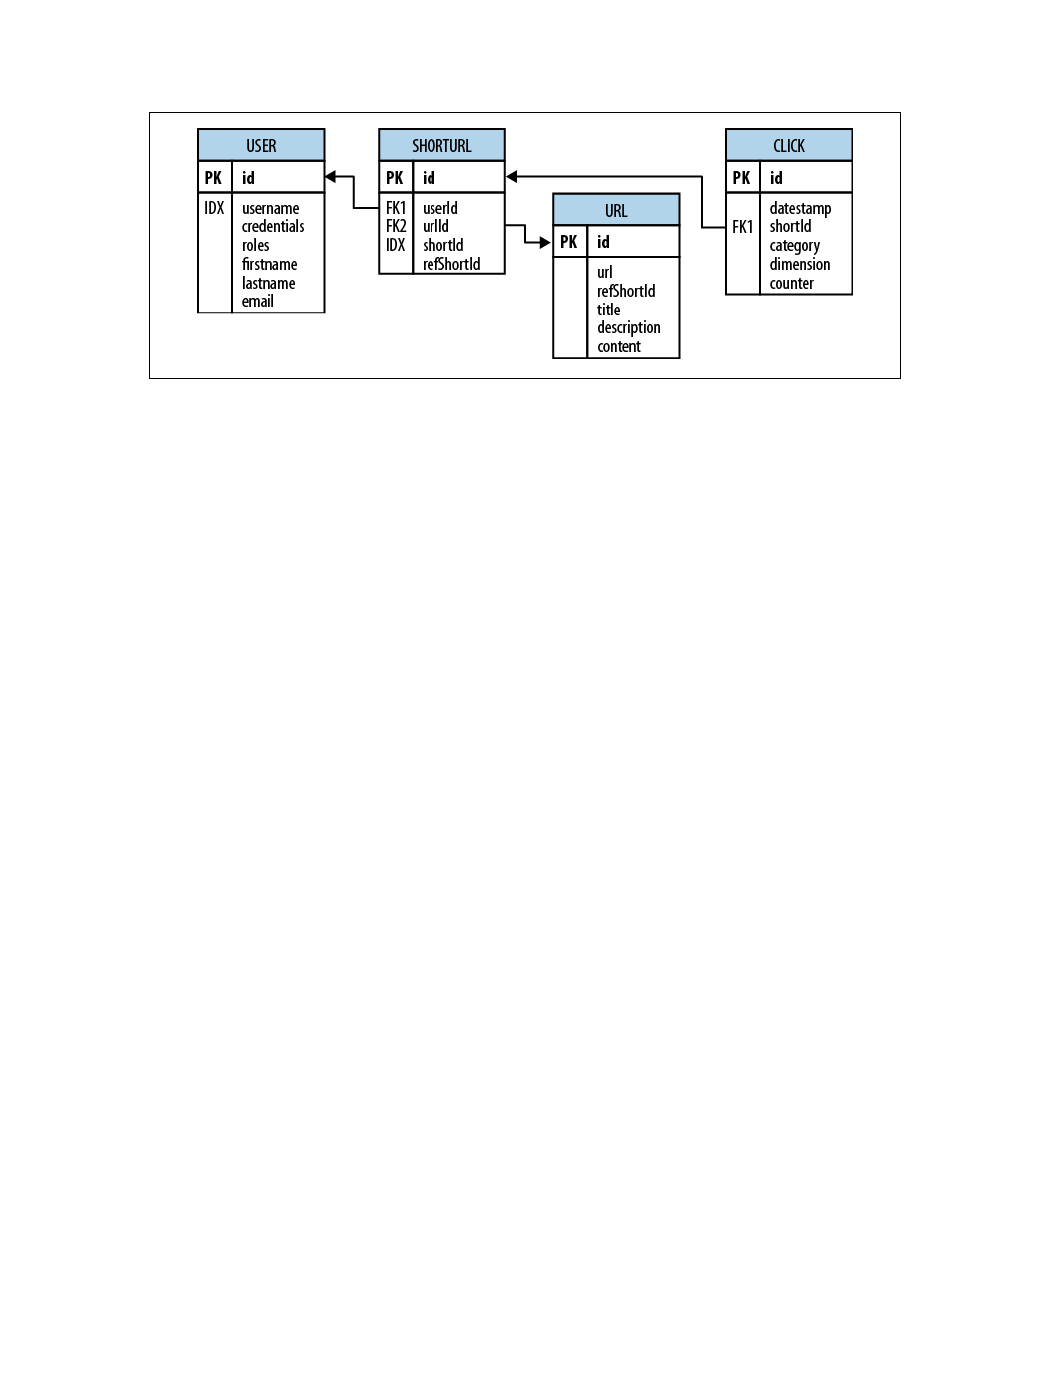
\includegraphics[scale=0.8]{./figures/hush-schema}
      \caption{The Hush Schema expressed as an ERD}
      \label{fig:hush_schema}
    \end{figure}

  \end{itemize}
}

\frame {\frametitle{The Problem with RDBMS}
  \begin{itemize}
  \item \textbf{Find all short URLs for a given user}
    \begin{itemize}
    \item \texttt{JOIN} \texttt{user} and \texttt{shorturl} tables
    \item Use the \texttt{WHERE} clause to select the given user
    \end{itemize}

    \vspace{20pt}

  \item \textbf{Stored Procedures}
    \begin{itemize}
    \item Consistently update data from multiple clients
    \item Underlying DB system guarantees coherency
    \end{itemize}

    \vspace{20pt}

  \item \textbf{Transactions}
    \begin{itemize}
    \item Make sure you can update tables in an \textit{atomic}
      fashion
    \item RDBMS $\to$ \textit{Strong Consistency} (ACID properties)
    \item \textit{Referential Integrity}
    \end{itemize}
  \end{itemize}
}

\frame {\frametitle{The Problem with RDBMS}
  \begin{itemize}
  \item \textbf{Scaling up to tens of thousands of users}
    \begin{itemize}
    \item Increasing pressure on the database server
    \item Adding more application servers is easy: they share their
      state on the same central DB
    \item CPU and I/O start to be a problem on the DB
    \end{itemize}

    \vspace{20pt}

  \item \textbf{Master-Slave architecture}
    \begin{itemize}
    \item Add DB server so that \texttt{READS} can be served in
      parallel
    \item Master DB takes all the writes (which are fewer in the Hush
      application)
    \item Slaves DB replicate Master DB and serve all reads (but you
      need a load balancer)
    \end{itemize}
  
  \end{itemize}
}

\frame {\frametitle{The Problem with RDBMS}
  \begin{itemize}
  \item \textbf{Scaling up to hundreds of thousands}
    \begin{itemize}
    \item \texttt{READS} are still the bottlenecks
    \item Slave servers begin to fall short in serving clients requests
    \end{itemize}

    \vspace{20pt}

  \item \textbf{Caching}
    \begin{itemize}
    \item Add a caching layer, e.g. Memcached or Redis
    \item Offload \texttt{READS} to a fast in-memory system
    \item[$\to$] You lose consistency guarantees
    \item[$\to$] Cache invalidation is critical for having DB and
      Caching layer consistent
    \end{itemize}

  \end{itemize}
}

\frame {\frametitle{The Problem with RDBMS}
  \begin{itemize}
  \item \textbf{Scaling up more}
    \begin{itemize}
    \item \texttt{WRITES} are the bottleneck
    \item The master DB is hit too hard by \texttt{WRITE} load
    \item \textit{Vertical scalability}: beef up your master server
    \item[$\to$] This becomes costly, as you may also have to replace
      your RDBMS
    \end{itemize}

    \vspace{20pt}

  \item \textbf{SQL \texttt{JOINs} becomes a bottleneck}
    \begin{itemize}
    \item Schema de-normalization
    \item Cease using stored procedures, as they become slow and eat
      up a lot of server CPU
    \item Materialized views (they speed up \texttt{READS})
    \item Drop secondary indexes as they slow down \texttt{WRITES}
    \end{itemize}
  \end{itemize}
}

\frame {\frametitle{The Problem with RDBMS}
  \begin{itemize}
  \item \textbf{What if your application needs to further scale up?}
    \begin{itemize}
    \item Vertical scalability vs. Horizontal scalability
    \end{itemize}

    \vspace{20pt}
    
    \item \textbf{Sharding}
      \begin{itemize}
      \item Partition your data across multiple databases
        \begin{itemize}
        \item Essentially you break horizontally your tables and ship
          them to different servers
        \item This is done using fixed boundaries
        \item[$\to$] Re-sharding to achieve load-balancing
        \end{itemize}
      \item[$\to$] This is an operational nightmare
      \item Re-sharding takes a huge toll on I/O resources
      \end{itemize}
  \end{itemize}
}

%%%%%%%%%%%%%%%%%%%%%%%%%%%%%%%%%%%%%%%%%%%%%%%%%%%%%%%%%%
\subsection{NOSQL}
%%%%%%%%%%%%%%%%%%%%%%%%%%%%%%%%%%%%%%%%%%%%%%%%%%%%%%%%%%
\frame {\frametitle{Non-Relational DataBases}
  \begin{itemize}
  \item \textbf{They originally do not support SQL}
    \begin{itemize}
    \item In practice, this is becoming a thin line to make the
      distinction
    \item One difference is in the data model
    \item Another difference is in the consistency model (ACID and
      transactions are generally sacrificed)
    \end{itemize}

    \vspace{20pt}

  \item \textbf{Consistency models and the CAP Theorem}
    \begin{itemize}
    \item Strict: all changes to data are atomic
    \item Sequential: changes to data are seen in the same order as
      they were applied
      \item Causal: causally related changes are seen in the same
        order
      \item Eventual: updates propagates through the system and
        replicas when in steady state
      \item Weak: no guarantee
    \end{itemize}

  \end{itemize}
}

\frame {\frametitle{Dimensions to classify NoSQL DBs}
  \begin{itemize}
  \item \textbf{Data model}
    \begin{itemize}
    \item How the data is stored: key/value, semi-structured,
      column-oriented, ...
    \item How to access data?
    \item Can the schema evolve over time?
    \end{itemize}

    \vspace{20pt}

  \item \textbf{Storage model}
    \begin{itemize}
    \item In-memory or persistent?
    \item How does this affect your access pattern?
    \end{itemize}

    \vspace{20pt}

  \item \textbf{Consistency model}
    \begin{itemize}
    \item Strict or eventual?
    \item This translates in how fast the system handles
      \texttt{READS} and \texttt{WRITES} \cite{Brewer01}
    \end{itemize}
  \end{itemize}
}

\frame {\frametitle{Dimensions to classify NoSQL DBs}
  \begin{itemize}
  \item \textbf{Physical Model}
    \begin{itemize}
    \item Distributed or single machine?
    \item How does the system scale?
    \end{itemize}

    \vspace{20pt}

  \item \textbf{Read/Write performance}
    \begin{itemize}
    \item Top-down approach: understands well the workload!
    \item Some systems are better for \texttt{READS}, other for \texttt{WRITES}
    \end{itemize}

    \vspace{20pt}

  \item \textbf{Secondary indexes}
    \begin{itemize}
    \item Does your workload require them?
    \item Can your system emulate them?
    \end{itemize}
  \end{itemize}
}

\frame {\frametitle{Dimensions to classify NoSQL DBs}
  \begin{itemize}
  \item \textbf{Failure Handling}
    \begin{itemize}
    \item How each data store handle server failures?
    \item Is it able to continue operating in case of failures?
      \begin{itemize}
      \item This is related to Consistency models and the CAP theorem
      \end{itemize}
      \item Does the system support ``hot-swap''?
    \end{itemize}

    \vspace{20pt}

  \item \textbf{Compression}
    \begin{itemize}
    \item Is the compression method pluggable?
    \item What type of compression?
    \end{itemize}

    \vspace{20pt}

  \item \textbf{Load Balancing}
    \begin{itemize}
    \item Can the storage system seamlessly balance load?
    \end{itemize}
  \end{itemize}
}

\frame {\frametitle{Dimensions to classify NoSQL DBs}
  \begin{itemize}
  \item \textbf{Atomic \texttt{read-modify-write}}
    \begin{itemize}
    \item Easy in a centralized system, difficult in a distributed one
    \item Prevent race conditions in multi-threaded or shared-nothing
      designs
    \item Can reduce client-side complexity
    \end{itemize}

    \vspace{20pt}

  \item \textbf{Locking, waits and deadlocks}
    \begin{itemize}
    \item Support for multiple client accessing data simultaneously
    \item Is locking available?
    \item Is it wait-free, hence deadlock free?
    \end{itemize}

    \vspace{20pt}

    \begin{beamerboxesrounded}{Impedance Match}

        ``One-size-fits-all'' has been long dismissed: need to find
        the perfect match for your problem.

    \end{beamerboxesrounded}

  \end{itemize}
}

%%%%%%%%%%%%%%%%%%%%%%%%%%%%%%%%%%%%%%%%%%%%%%%%%%%%%%%%%%
\subsection{Denormalization}
%%%%%%%%%%%%%%%%%%%%%%%%%%%%%%%%%%%%%%%%%%%%%%%%%%%%%%%%%%
\frame {\frametitle{Database (De-)Normalization}
  \begin{itemize}
  \item \textbf{Schema design at scale}
    \begin{itemize}
    \item A good methodology is to apply the DDI principle \cite{Salmen09}
      \begin{itemize}
      \item Denormalization
      \item Duplication
      \item Intelligent Key design
      \end{itemize}
    \end{itemize}

    \vspace{20pt}

  \item \textbf{Denormalization}
    \begin{itemize}
    \item Duplicate data in more than one table such that at
      \texttt{READ} time no further aggregation is required
    \end{itemize}

    \vspace{20pt}

  \item \textbf{Next: an example based on Hush}
    \begin{itemize}
    \item How to convert a classic relational data model to one that
      fits HBase
    \item This example will be covered in the LAB session 3
    \end{itemize}
  \end{itemize}
}

\frame {\frametitle{Example: Hush - from RDBMS to HBase}
    \begin{figure}[h]
      \centering
      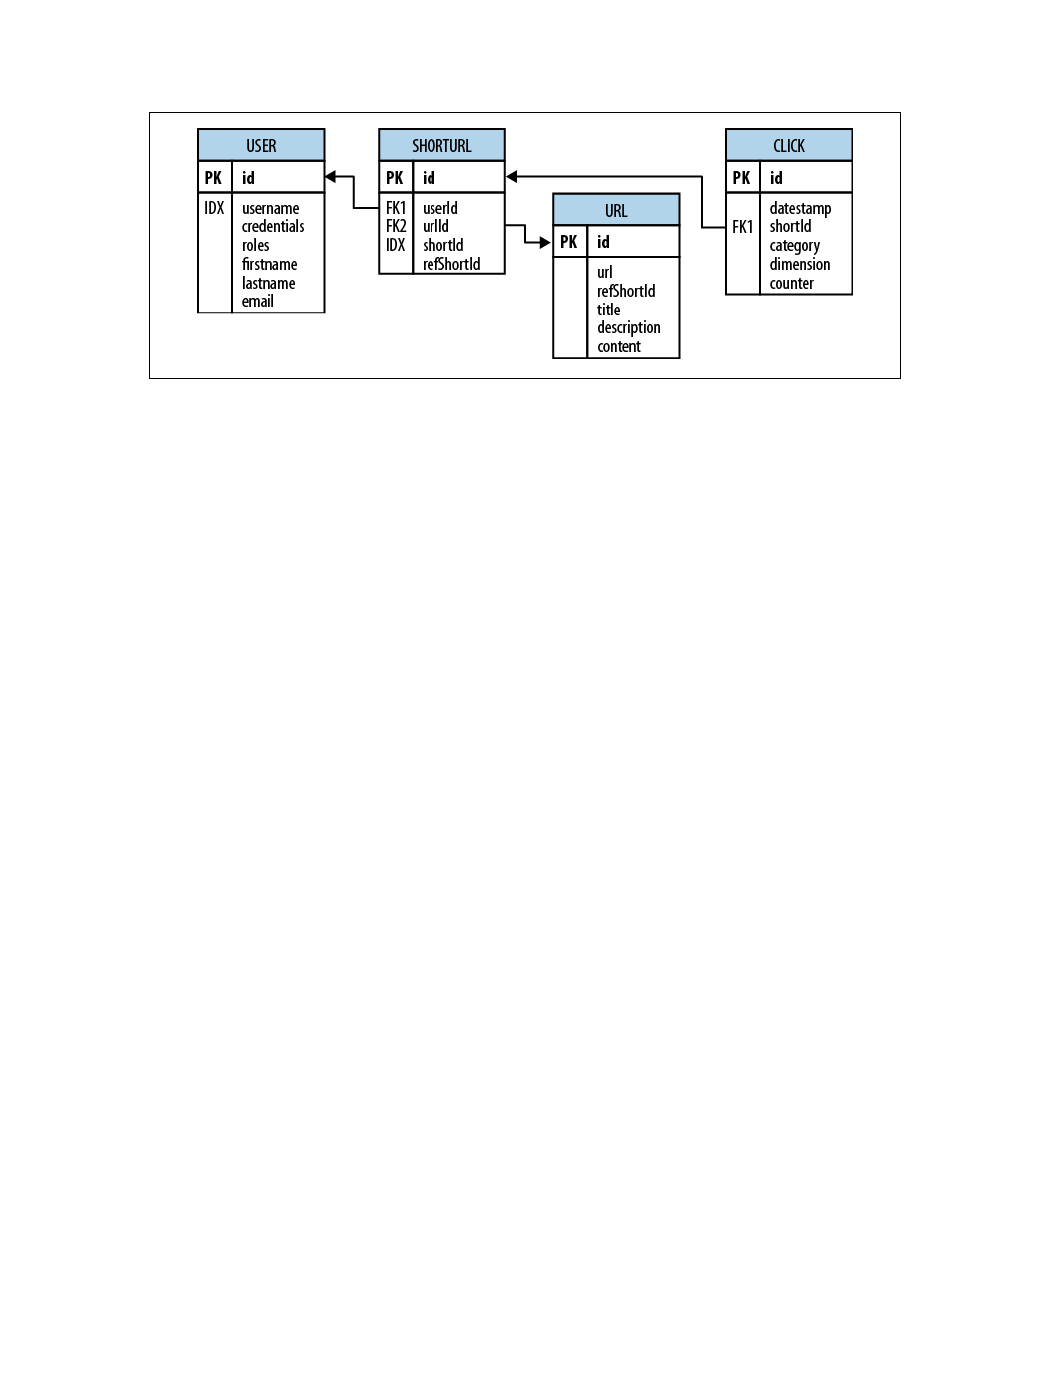
\includegraphics[scale=0.6]{./figures/hush-schema}
      \caption{The Hush Schema expressed as an ERD}
      \label{fig:hush_schema}
    \end{figure}

    \begin{itemize}
    \item \texttt{shorturl} table: contains the short URL
    \item \texttt{click} table: contains click tracking, and other
      statistics, aggregated on a daily basis (essentially, a counter)
    \item \texttt{user} table: contains user information
    \item \texttt{URL} table: contains a replica of the page linked to
      a short URL, including META data and content (this is done for
      batch analysis purposes)
    \end{itemize}
}

\frame {\frametitle{Example: Hush - from RDBMS to HBase}
    \begin{figure}[h]
      \centering
      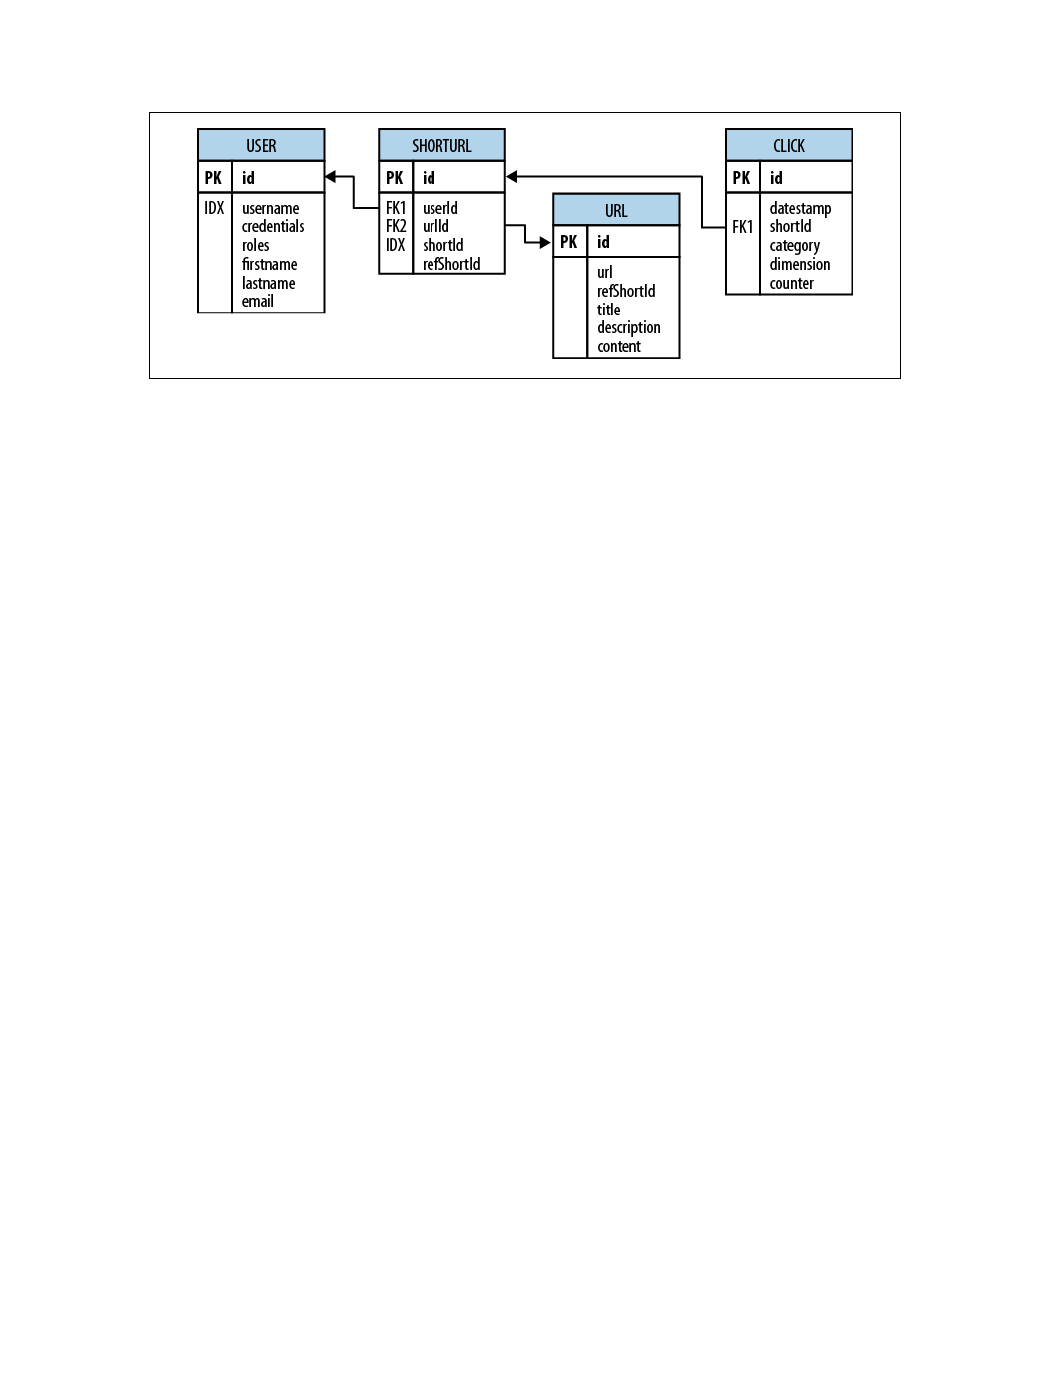
\includegraphics[scale=0.6]{./figures/hush-schema}
      \caption{The Hush Schema expressed as an ERD}
      \label{fig:hush_schema}
    \end{figure}

    \begin{itemize}
    \item \texttt{user} table is indexed on the \texttt{username}
      field, for fast user lookup
    \item \texttt{shorturl} table is indexed on the short URL
      (\texttt{shortId}) field, for fast short URL lookup
   \end{itemize}
}

\frame {\frametitle{Example: Hush - from RDBMS to HBase}
    \begin{figure}[h]
      \centering
      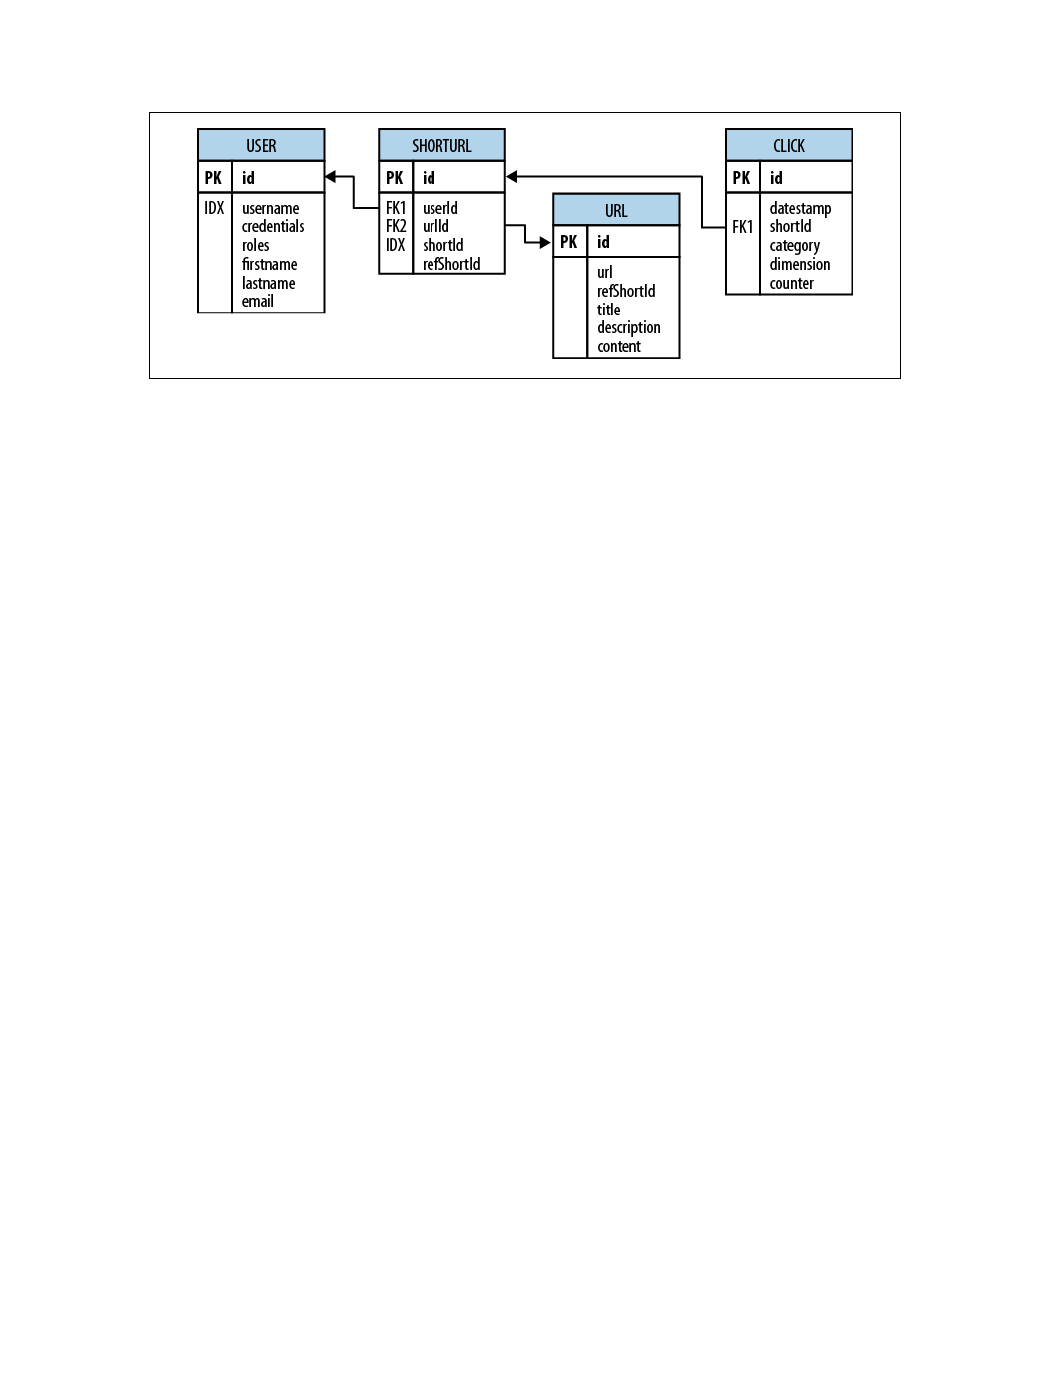
\includegraphics[scale=0.6]{./figures/hush-schema}
      \caption{The Hush Schema expressed as an ERD}
      \label{fig:hush_schema}
    \end{figure}

    \begin{itemize}
    \item \texttt{shorturl} and \texttt{user} tables are related
      through a foreign key relation on the \texttt{userId}
    \item \texttt{URL} table is related to \texttt{shorturl} table
      with a foreign key on the URL id
    \item \texttt{click} table is related to \texttt{shorturl} table
      with a foreign key on the short URL id
    \item NOTE: a web page is stored only once (even if multiple users
      link to it), but each users maintain separate statistics
   \end{itemize}
}

\frame {\frametitle{Example: Hush - from RDBMS to HBase}
  \begin{columns}[c]
    \column{6cm}

    \vspace{-10pt}

    \begin{figure}[h]
      \centering
      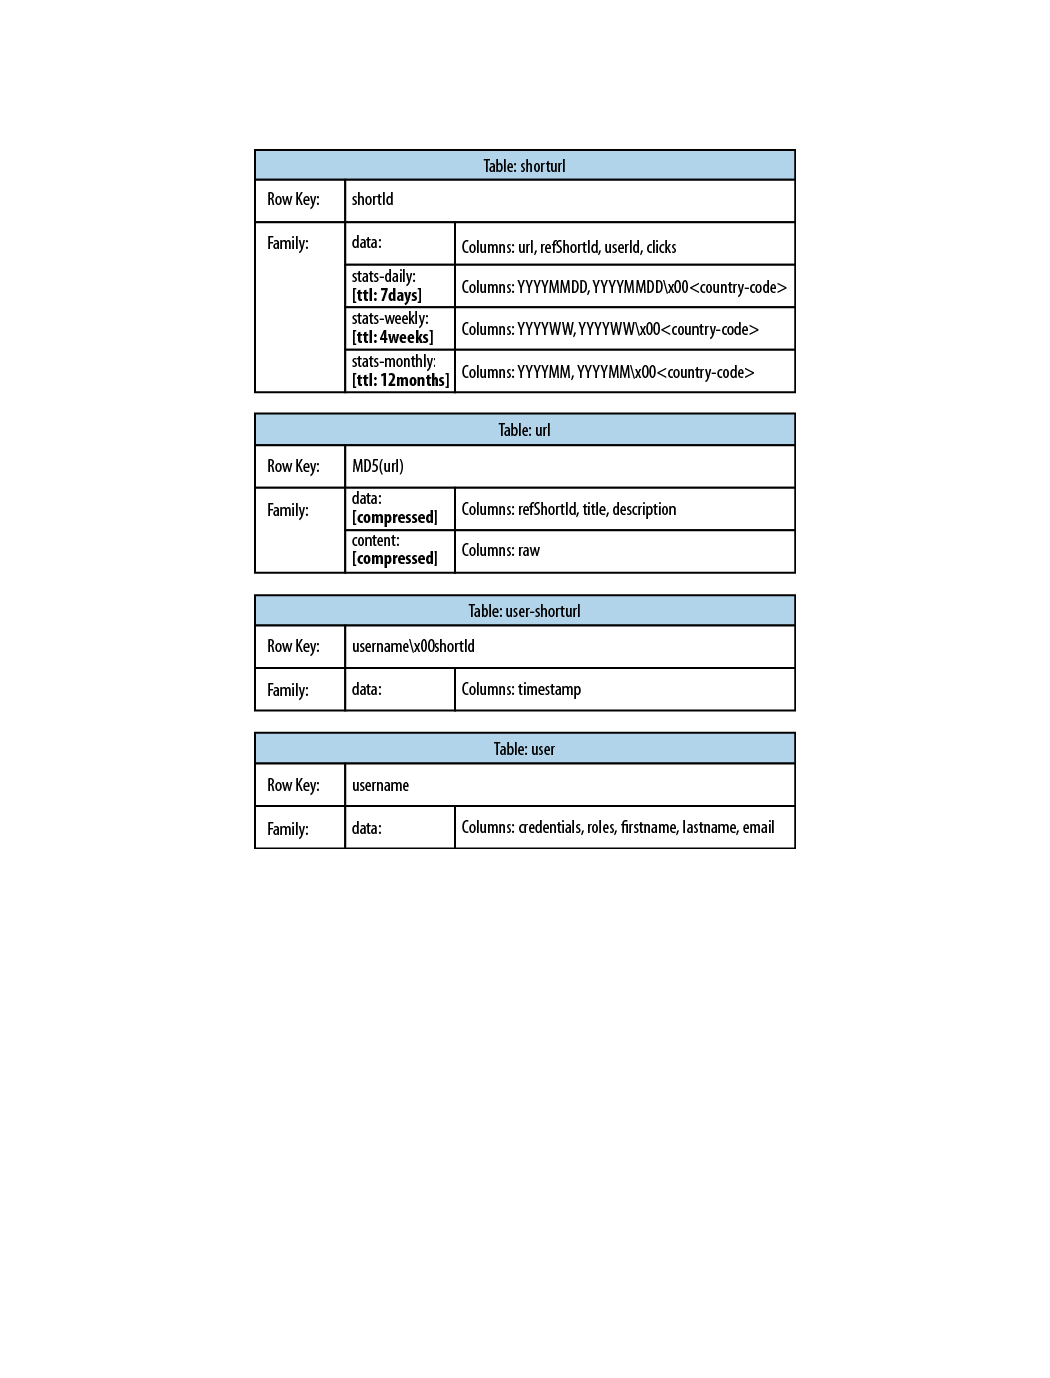
\includegraphics[scale=0.6]{./figures/hush-hbase}
      \caption{The Hush Schema in HBase}
      \label{fig:hush_schema}
    \end{figure}
    
    
    \column{6cm}
    \begin{itemize}
    \item \texttt{shorturl} table: stores each short URL, usage
      statistics (various time-ranges in separate
      \textit{column-families} with distinct \textit{TTL} settings)
      \begin{itemize}
      \item Note the dimensional postfix appended to the time information
      \end{itemize}
      
      \vspace{20pt}
      
    \item \texttt{url} table: stores the downloaded page, and the
      extracted details
      \begin{itemize}
      \item This table uses compression
      \end{itemize}
    \end{itemize}
  \end{columns}
}

\frame {\frametitle{Example: Hush - from RDBMS to HBase}
  \begin{columns}[c]
    \column{6cm}

    \vspace{-10pt}

    \begin{figure}[h]
      \centering
      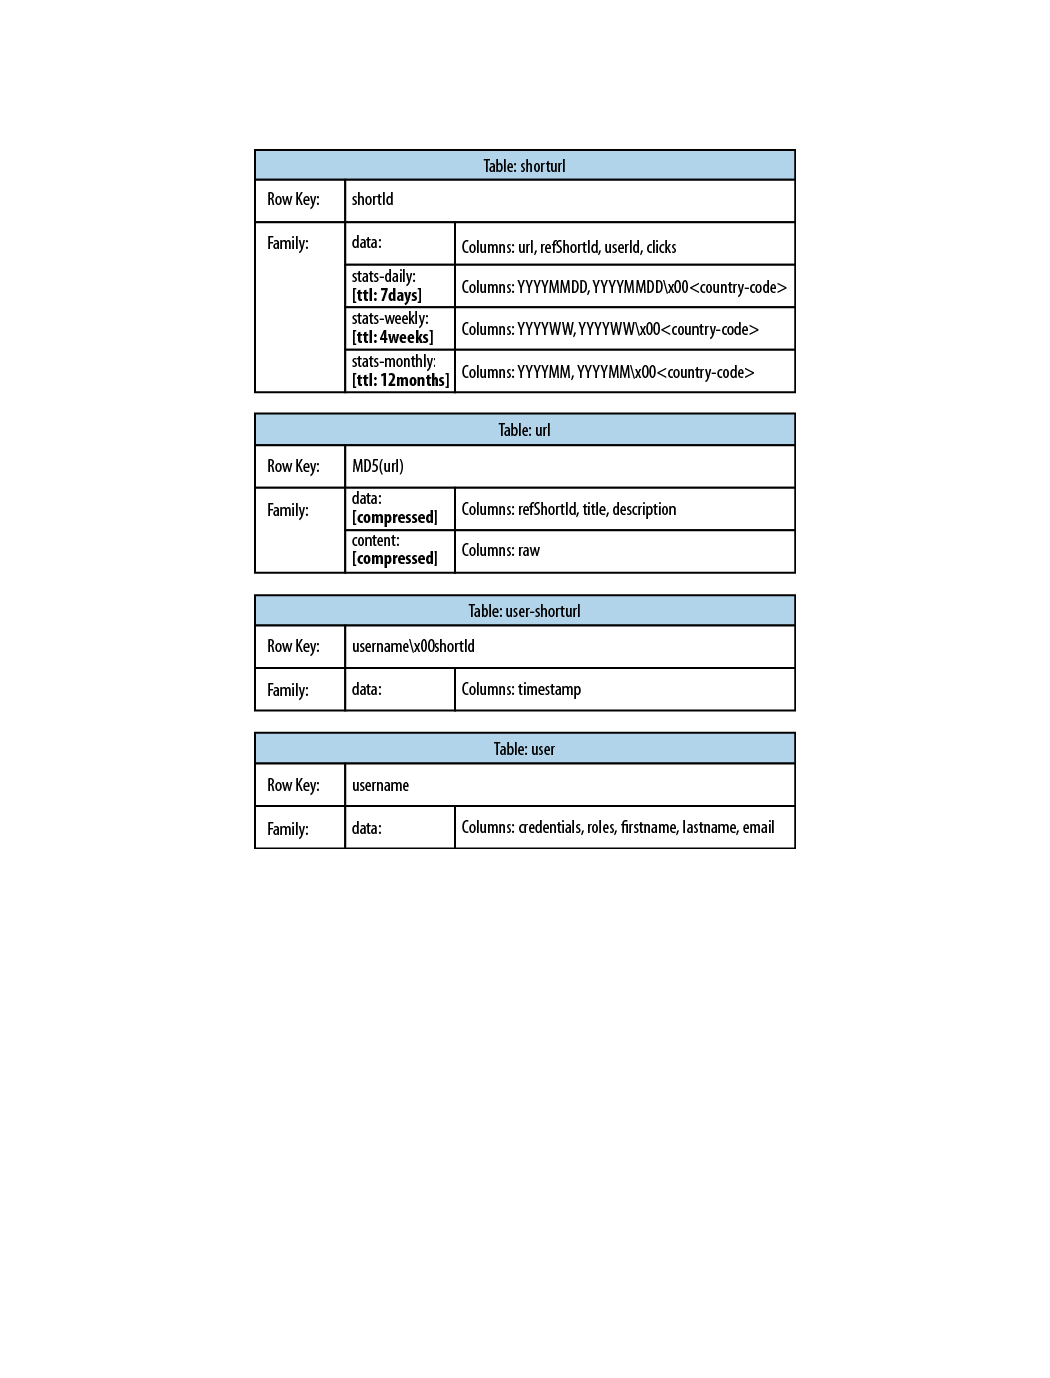
\includegraphics[scale=0.6]{./figures/hush-hbase}
      \caption{The Hush Schema in HBase}
      \label{fig:hush_schema}
    \end{figure}
        
    \column{6cm}
    \begin{itemize}
    \item \texttt{user-shorturl} table: this is a lookup table
      (basically an index) to find all shortIDs for a given user
      \begin{itemize}
      \item Note that this table is filled at \textit{insert time},
        it's not automatically generated by HBase
      \end{itemize}

      \vspace{20pt}

    \item \texttt{user} table: stores user details
    \end{itemize}
  \end{columns}
}

\frame {\frametitle{Example: Hush - RDBMS vs HBase}
  \begin{itemize}
  \item \textbf{Same number of tables}
    \begin{itemize}
    \item Their meaning is different
    \item \texttt{click} table has been absorbed by the
      \texttt{shorturl} table
    \item statistics are stored with the date as the key, so that they
      can be accessed \textit{sequentially}
    \item The \texttt{user-shorturl} table is replacing the foreign
      key relationship, making user-related lookups faster
    \end{itemize}

    \vspace{20pt}

  \item \textbf{Normalized vs. De-normalized data}
    \begin{itemize}
    \item Wide tables and column-oriented design eliminates
      \texttt{JOINs}
    \item \textit{Compound keys} are essential
    \item Data partitioning is based on keys, so a proper
      understanding thereof is essential
    \end{itemize}
  \end{itemize}
}

%%%%%%%%%%%%%%%%%%%%%%%%%%%%%%%%%%%%%%%%%%%%%%%%%%%%%%%%%%
\subsection{HBase Sketch}
%%%%%%%%%%%%%%%%%%%%%%%%%%%%%%%%%%%%%%%%%%%%%%%%%%%%%%%%%%
\frame {\frametitle{HBase building blocks}
  \begin{itemize}
  \item \textbf{The backdrop: BigTable}
    \begin{itemize}
    \item GFS, The Google FileSystem \cite{Ghemawat2003}
    \item Google MapReduce \cite{Dean2004}
    \item BigTable \cite{Chang2006}
    \end{itemize}

    \vspace{20pt}

  \item \textbf{What is BigTable?}
    \begin{itemize}
    \item BigTable is a distributed storage system for managing
      structured data designed to scale to a very large size
    \item BigTable is a sparse, distributed, persistent
      multi-dimensional sorted map
    \end{itemize}
    
    \vspace{20pt}
    
  \item \textbf{What is HBase?}
    \begin{itemize}
    \item Essentially it's an open-source version of BigTable
    \item Differences listed in \cite{George2011}
    \end{itemize}
  \end{itemize}
}

\frame {\frametitle{HBase building blocks}
  \begin{beamerboxesrounded}{}
    Tables, Rows, Columns, and Cells
  \end{beamerboxesrounded}

  \begin{itemize}
  \item \textbf{The most basic unit in HBase is a \textit{column}}
    \begin{itemize}
    \item Each column may have multiple versions, with each distinct
      value contained in a separate \textit{cell}
    \item One or more columns form a \textit{row}, that is addressed uniquely
      by a \textit{row key}
    \end{itemize}

    \vspace{20pt}
    
  \item A table is a collection of rows
    \begin{itemize}
    \item All rows are always \textit{sorted lexicographically} by
      their row key
    \end{itemize}
  \end{itemize}
  \begin{figure}[h]
    \centering
    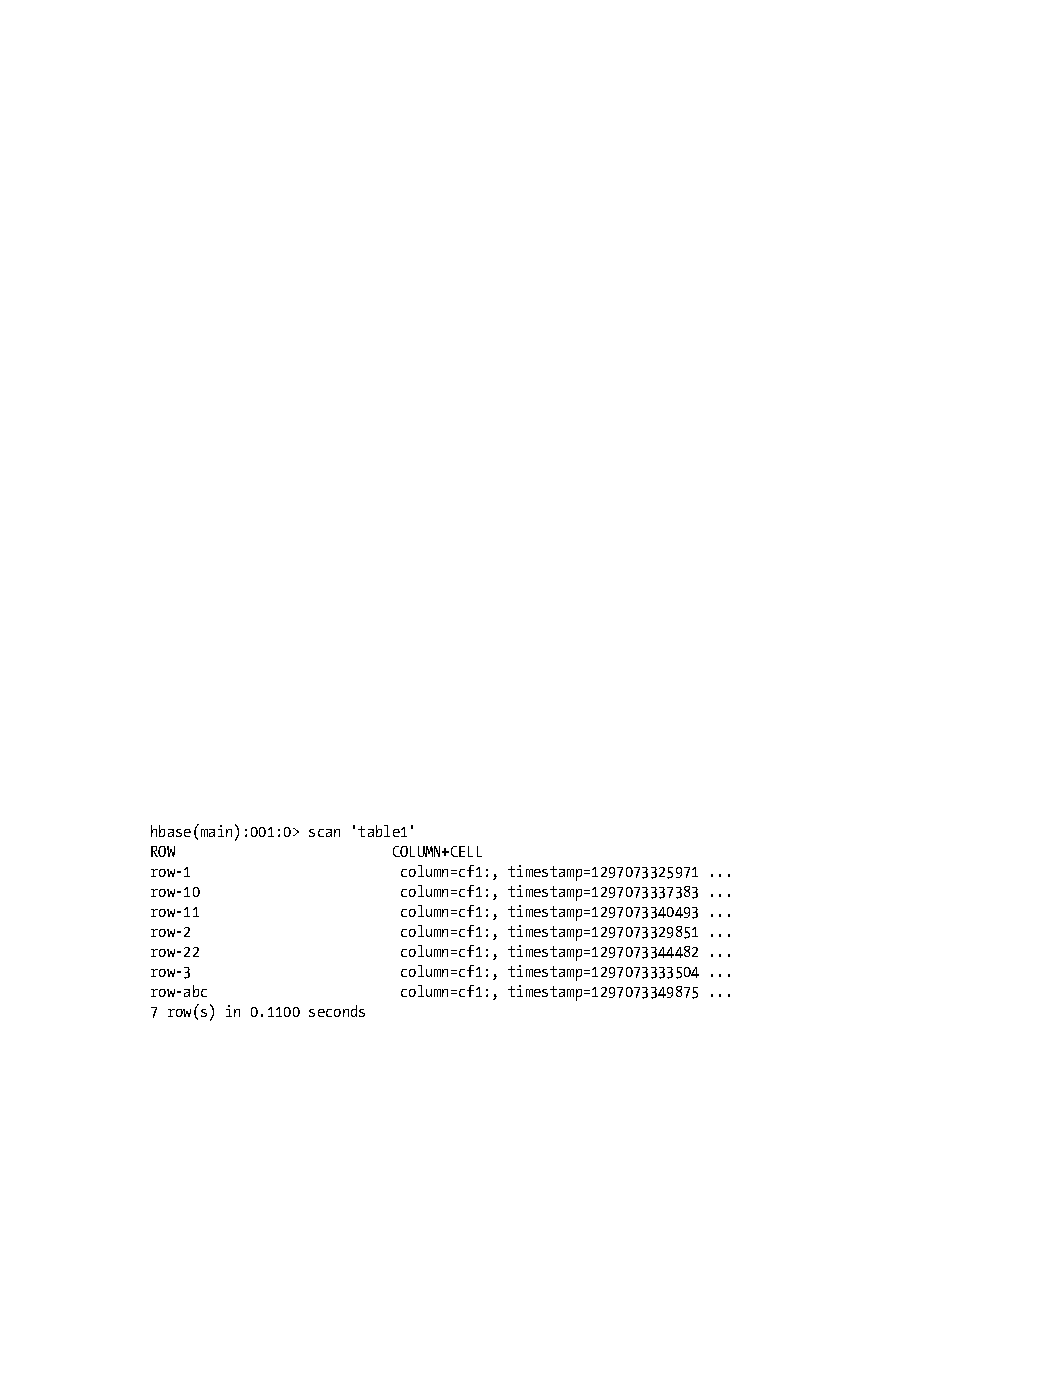
\includegraphics[scale=0.8]{./figures/lexi-sort}
  \end{figure}

}

\frame {\frametitle{HBase building blocks}
  \begin{beamerboxesrounded}{}
    Tables, Rows, Columns, and Cells
  \end{beamerboxesrounded}

  \begin{itemize}
  \item \textbf{Lexicographical ordering of row keys}
    \begin{itemize}
    \item Keys are compared on a binary level, byte by byte, from left
      to right
    \item This can be thought of as a primary index on the row key!
    \item Row keys are \textit{always unique}
    \item Row keys can be any \textit{arbitrary array of bytes}
    \end{itemize}

    \vspace{20pt}

  \item \textbf{Columns}
    \begin{itemize}
    \item Rows are composed of columns
    \item Can have millions of columns
    \item Can be compressed or tagged to stay in memory
    \end{itemize}
  \end{itemize}
}

\frame {\frametitle{HBase building blocks}
  \begin{beamerboxesrounded}{}
    Tables, Rows, Columns, and Cells
  \end{beamerboxesrounded}

  \begin{itemize}
  \item \textbf{Column Families}
    \begin{itemize}
    \item Columns are grouped into \textit{column families}
    \item[$\to$] Semantical boundaries between data
    \item Column families and columns stored together in the same
      low-level storage file, called an \textit{HFile}
    \item Defined when table is created
    \item Should not be changed too often
    \item The number of column families should be reasonable
      [{\color{red}WHY?}]
    \item Column family name composed by printable characters
    \end{itemize}

    \vspace{20pt}

  \item \textbf{References to columns}
    \begin{itemize}
    \item Column ``name'' is called \texttt{qualifier}, and can be any
      arbitrary number of bytes
    \item Reference: \texttt{family:qualifier} (also called the {\color{red}column key})
    \end{itemize}

  \end{itemize}

}

\frame {\frametitle{HBase building blocks}
  \begin{beamerboxesrounded}{}
    Tables, Rows, Columns, and Cells
  \end{beamerboxesrounded}

  \begin{itemize}
  \item \textbf{A note on the \texttt{NULL} value}
    \begin{itemize}
    \item In RDBMS \texttt{NULL} cells need to be set and occupy space
    \item In HBase, \texttt{NULL} cells or columns are simply not stored
    \end{itemize}

    \vspace{20pt}

  \item \textbf{A \textit{cell}}
    \begin{itemize}
    \item Every column value, or cell, is timestamped (implicitly or
      explicitly)
      \begin{itemize}
      \item This can be used to save multiple versions of a value that
        changes over time
      \item Versions are stored in decreasing timestamp, most recent first
      \end{itemize}
    \item Cell versions can be constrained by \textit{predicate
        deletions}
      \begin{itemize}
      \item Keep only values from the last week
      \end{itemize}
    \end{itemize}
  \end{itemize}
}

\frame {\frametitle{HBase building blocks}
  \begin{beamerboxesrounded}{}
    Tables, Rows, Columns, and Cells
  \end{beamerboxesrounded}
  \begin{itemize}
  \item \textbf{Access to data}
    \begin{itemize}
    \item \texttt{(Table, RowKey, Family, Column, Timestamp) $\to$
        Value}
    \item \texttt{SortedMap<RowKey, List<SortedMap<Column, List<Value,
        Timestamp$>\,>\,>\,>$}
    \item[]
    \item The first \texttt{SortedMap} is the table, containing a
      \texttt{List} of column families
    \item The families contain another \texttt{SortedMap}, representing columns
      and a \texttt{List} of value, timestamp tuples
    \end{itemize}

    \vspace{20pt}
    
  \item \textbf{A note on consistency:}
    \begin{itemize}
    \item Row data access is \textbf{atomic} and includes any number
      of columns
    \item There is no further guarantee or transactional feature
      spanning multiple rows
    \item[$\to$] HBase is strictly consistent
    \end{itemize}

  \end{itemize}
}

\frame {\frametitle{HBase building blocks}
  \begin{beamerboxesrounded}{}
    Automatic Sharding
  \end{beamerboxesrounded}

  \begin{itemize}
  \item \textbf{Region}
    \begin{itemize}
    \item This is the basic unit of scalability and load balancing
    \item Regions are contiguous ranges of rows ``stored together'' $\to$
      they are the equivalent of \textit{range partitions} in sharded RDBMS
    \item Regions are \textit{dynamically split} by the system when
      they become too large
    \item Regions can also be merged to reduce the number of storage files
    \end{itemize}
    
    \vspace{20pt}

  \item \textbf{Regions in practice}
    \begin{itemize}
    \item Initially, there is one region
    \item System monitors region size: if a threshold is attained,
      \texttt{SPLIT}
      \begin{itemize}
      \item Regions are split in two at the \textit{middle key}
      \item This creates roughly two equivalent (in size) regions
      \end{itemize}
    \end{itemize}
  \end{itemize}
}

\frame {\frametitle{HBase building blocks}
  \begin{beamerboxesrounded}{}
    Automatic Sharding
  \end{beamerboxesrounded}
  
  \begin{itemize}
  \item \textbf{Region Servers}
    \begin{itemize}
    \item Each region is served by \textit{exactly one Region Server}
    \item Region servers can serve multiple regions
    \item The number of region servers and their sizes depend on the
      capability of a single region server
    \end{itemize}
    
    \vspace{20pt}
    
  \item \textbf{Server failures}
    \begin{itemize}
    \item Regions allow for fast recovery upon failure
    \item Fine-grained Load Balancing is also achieved using regions
      as they can be easily moved across servers
    \end{itemize}
  \end{itemize}
}

\frame {\frametitle{HBase building blocks}
  \begin{beamerboxesrounded}{}
    Storage API
  \end{beamerboxesrounded}
 
  \begin{itemize}
  \item \textbf{No support for SQL}
    \begin{itemize}
    \item CRUD operations using a standard API, available for many
      ``clients''
    \item Data access is not declarative but imperative
    \end{itemize}
    
    \vspace{20pt}
    
  \item \textbf{Scan API}
    \begin{itemize}
    \item Allows for fast iteration over ranges of rows
    \item Allows to limit the number and which column are returned
    \item Allows to control the version number of each cell
    \end{itemize}
    
    \vspace{20pt}
    
  \item \textbf{Read-modify-write API}
    \begin{itemize}
    \item HBase supports single-row transactions
    \item Atomic read-modify-write on data stored in a single row key
    \end{itemize}
  \end{itemize}
}

\frame {\frametitle{HBase building blocks}
  \begin{beamerboxesrounded}{}
    Storage API
  \end{beamerboxesrounded}

  \begin{itemize} 
  \item \textbf{Counters}
    \begin{itemize}
    \item Values can be interpreted as counters and \textbf{updated
        atomically}
    \item Can be read and modified in one operation
    \item[$\to$] Implement global, strictly consistent, sequential counters
    \end{itemize}

    \vspace{20pt}
    
  \item \textbf{Coprocessors}
    \begin{itemize}
    \item These are equivalent to stored-procedures in RDBMS
    \item Allow to push user code in the address space of the server
    \item Access to server local data
    \item Implement lightweight batch jobs, data pre-processing, data summarization
    \end{itemize}
    
  \end{itemize}
}

\frame {\frametitle{HBase building blocks}
  \begin{beamerboxesrounded}{}
    HBase implementation
  \end{beamerboxesrounded}

  \begin{itemize}
  \item \textbf{Data Storage}
    \begin{itemize}
    \item \textit{Store} files are called \texttt{HFiles}
    \item Persistent and ordered \textbf{immutable} maps from key to
      value
    \item Internally implemented as sequences of blocks with an index
      at the end
    \item Index is loaded when the \texttt{HFile} is opened and kept in memory
    \end{itemize}

    \vspace{20pt}

  \item \textbf{Data lookups}
    \begin{itemize}
    \item Since \texttt{HFiles} have a block index, lookup can be done
      with a single disk seek
    \item First, the block possibly containing a given lookup key is
      determined with a \textbf{binary search} in the in-memory index
    \item Then a block read is performed to find the actual key
    \end{itemize}

    \vspace{20pt}

  \item \textbf{Underlying file system}
    \begin{itemize}
    \item Many are supported, usually HBase deployed on top of HDFS
    \end{itemize}

  \end{itemize}
}

\frame {\frametitle{HBase building blocks}
  \begin{beamerboxesrounded}{}
    HBase implementation
  \end{beamerboxesrounded}

  \begin{itemize}
  \item \textbf{\texttt{WRITE} operation}
    \begin{itemize}
    \item First, data is written to a commit log, called WAL
      (write-ahead-log)
    \item Then data is moved into memory, in a structure called
      \texttt{memstore}
    \item When the size of the \texttt{memstore} exceeds a given
      threshold it is flushed to an \texttt{HFile} to disk
    \end{itemize}

    \vspace{20pt}

  \item \textbf{How can HBase write, while serving \texttt{READS} and
      \texttt{WRITES}?}
    \begin{itemize}
    \item Rolling mechanism
      \begin{itemize}
      \item new/empty slots in the \texttt{memstore}
        take the updates
      \item old/full slots are flushed to disk
      \end{itemize}
    \item Note that data in \texttt{memstore} is sorted by keys, matching what
      happens in the \texttt{HFiles}
    \end{itemize}

    \vspace{20pt}

  \item \textbf{Data Locality}
    \begin{itemize}
    \item Achieved by the system looking up for server hostnames
    \item Achieved through intelligent key design
    \end{itemize}
  \end{itemize}
}

\frame {\frametitle{HBase building blocks}
  \begin{beamerboxesrounded}{}
    HBase implementation
  \end{beamerboxesrounded}

  \begin{itemize}
  \item \textbf{Deleting data}
    \begin{itemize}
    \item Since HFiles are immutable, how can we delete data?
    \item A delete marker (also known as \textit{tombstone marker}) is
      written to indicate that a given key is deleted
    \item During the read process, data marked as deleted is skipped
    \item Compactions (see next slides) finalize the deletion process
    \end{itemize}

    \vspace{20pt}

  \item \textbf{\texttt{READ} operation}
    \begin{itemize}
    \item Merge of what is stored in the \texttt{memstores} (data that
      is not on disk) and in the \texttt{HFiles}
    \item The WAL is never used in the \texttt{READ} operation
    \item Several API calls to read, scan data
    \end{itemize}

  \end{itemize}
}

\frame {\frametitle{HBase building blocks}
  \begin{beamerboxesrounded}{}
    HBase implementation
  \end{beamerboxesrounded}
  \begin{itemize}
  \item \textbf{Compactions}
    \begin{itemize}
    \item Flushing data from \texttt{memstores} to disk implies the creation of
      new \texttt{HFiles} each time
    \item[$\to$] We end up with many (possibly small) files
    \item[$\to$] We need to do housekeeping [{\color{red}WHY?}]
    \end{itemize}

    \vspace{20pt}

  \item \textbf{Minor Compaction}
    \begin{itemize}
    \item Rewrites small \texttt{HFiles} into fewer, larger
      \texttt{HFiles}
    \item This is done using an $n$-way merge\footnote{What is MergeSort?}
    \end{itemize}
    \vspace{20pt}

  \item \textbf{Major Compaction}
    \begin{itemize}
    \item Rewrites all files within a column family or a region in a
      new one
    \item Drop deleted data
    \item Perform predicated deletion (e.g. delete old data)
    \end{itemize}
  \end{itemize}
}

\frame {\frametitle{HBase: a glance at the architecture}
  \begin{figure}[h]
    \centering
    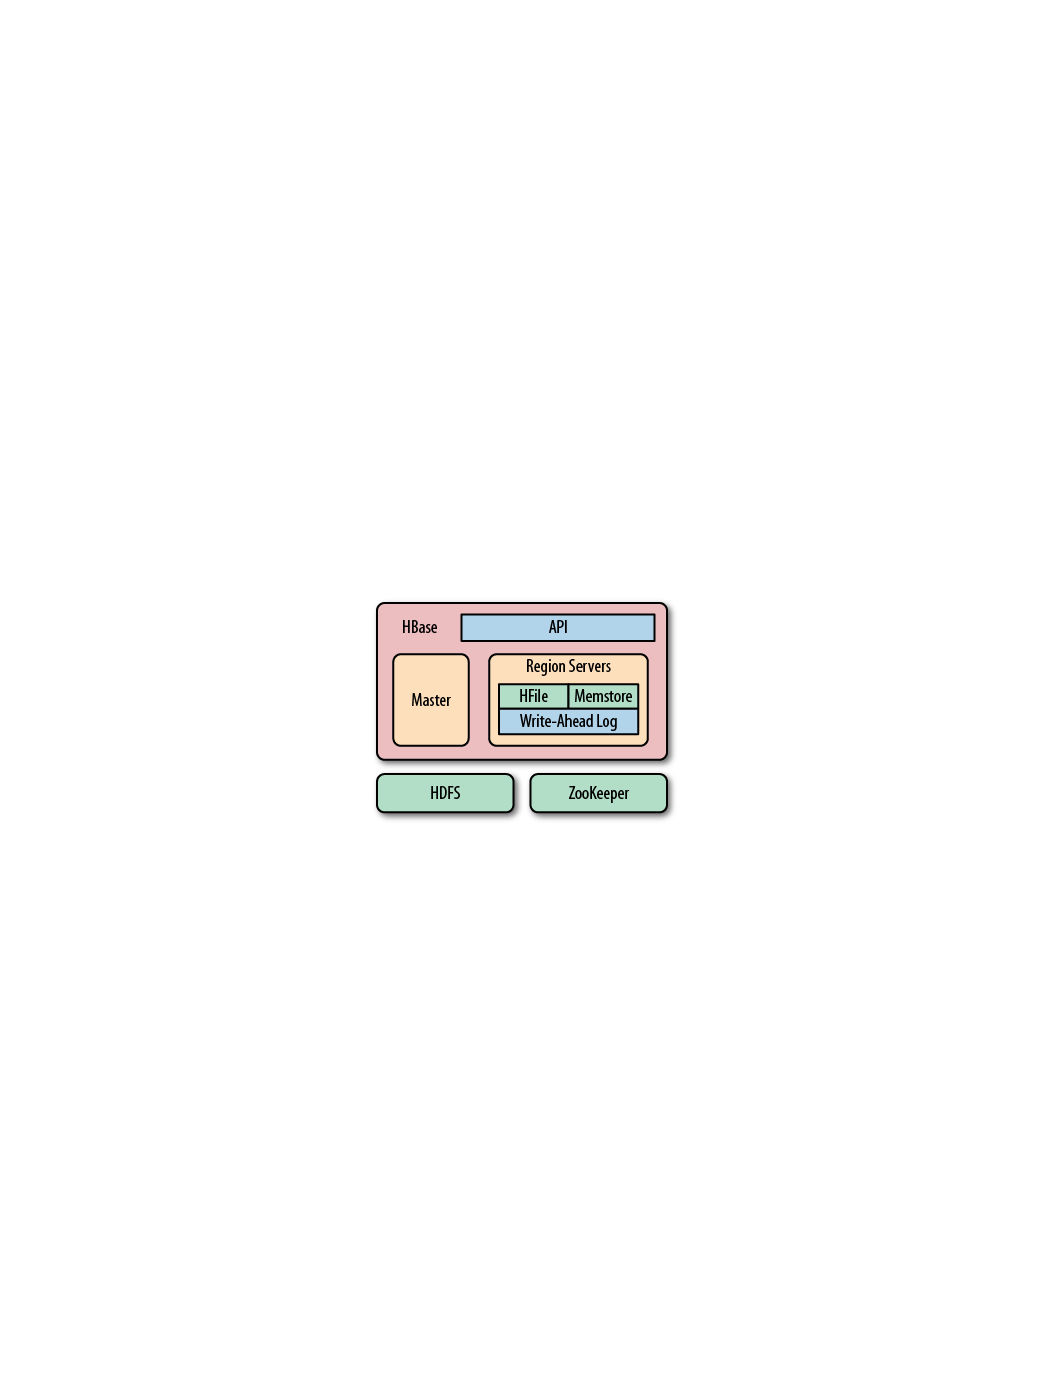
\includegraphics[scale=0.8]{./figures/hbase-arch}
  \end{figure}

  \begin{itemize}
  \item \textbf{Master node: \texttt{HMaster}}
    \begin{itemize}
    \item Assigns regions to region servers using ZooKeeper
    \item Handles load balancing
    \item Not part of the data path
    \item Holds metadata and schema
    \end{itemize}

    \vspace{10pt}

  \item \textbf{Region Servers}
    \begin{itemize}
    \item Handle \texttt{READs} and \texttt{WRITEs}
    \item Handle region splitting
    \end{itemize}
  \end{itemize}
}


\subsection{Architecture}
%%%%%%%%%%%%%%%%%%%%%%%%%%%%%%%%%%%%%%%%%%%%%%%%%%%%%%%%%%
\begin{frame}
  \begin{beamerboxesrounded}{}
	\begin{center}

\vspace{20pt}

		Architecture

\vspace{20pt}

	\end{center}    
  \end{beamerboxesrounded}
\end{frame}


%%%%%%%%%%%%%%%%%%%%%%%%%%%%%%%%%%%%%%%%%%%%%%%%%%%%%%%%%%
\subsection{Seek vs. Transfer}
%%%%%%%%%%%%%%%%%%%%%%%%%%%%%%%%%%%%%%%%%%%%%%%%%%%%%%%%%%
\frame {\frametitle{Seek vs. Transfer}
  \begin{itemize}
  \item \textbf{Fundamental difference between RDBMS and alternatives}
    \begin{itemize}
    \item B+Trees
    \item Log-Structured Merge Trees
    \end{itemize}

    \vspace{20pt}

  \item \textbf{Seek vs. Transfer}
    \begin{itemize}
    \item Random access to individual cells
    \item Sequential access to data
    \end{itemize}
  \end{itemize}
}

\frame {\frametitle{B+ Trees}
  \begin{itemize}
  \item \textbf{Dynamic, multi-level indexes}
    \begin{itemize}
    \item Efficient insertion, lookup and deletion
    \item {\color{red}Q: What's the difference between a B+ Tree and a
        Hash Table?}
    \item Frequent updates may imbalance the trees $\to$ Tree
      optimization and re-organization is required (which is a costly operation)
    \end{itemize}

    \vspace{20pt}

  \item \textbf{Bounds on \textit{page size}}
    \begin{itemize}
    \item Number of keys in each branch
    \item Larger fanout compared to binary trees
    \item Lower number of I/O operations to find a specific key
    \end{itemize}

    \vspace{20pt}

  \item \textbf{Support for range scans}
    \begin{itemize}
    \item Leafs are linked and represent an in-order list of all keys
    \item No costly tree-traversal algorithms required
    \end{itemize}
  \end{itemize}
}

\frame {\frametitle{LSM-Trees}
  \begin{itemize}
  \item \textbf{Data flow}
    \begin{itemize}
    \item Incoming data is first stored in a logfile,
      \textit{sequentially}
    \item Once the log has the modification saved, data is pushed in
      memory
      \begin{itemize}
    \item In-memory store holds most recent updates for fast lookup
      \end{itemize}
    \item When memory is ``full'', data is flushed in a store file to
      disk, as a sorted list of \texttt{key $\to$ record} pair
    \item At this point, the log file can be thrown away
    \end{itemize}

    \vspace{20pt}

  \item \textbf{How store files are arranged}
    \begin{itemize}
    \item Similar idea of a B+ Tree, but optimized for sequential disk
      access
    \item All nodes of the tree try to be filled up completely
    \item Updates are done in a \textbf{rolling merge} fashion
      \begin{itemize}
      \item The system packs existing on-disk multi-page blocks with
        in-memory data until the block reaches full capacity
      \end{itemize}
    \end{itemize}
  \end{itemize}
}

\frame {\frametitle{LSM-Trees}
  \begin{itemize}
  \item \textbf{Clean-up process}
    \begin{itemize}
    \item As flushes take place over time, a lot of store files are
      created
    \item Background process aggregates files into larger ones to
      limit disk seeks
    \item All store files are always sorted by key $\to$ no
      re-ordering required to fit new keys in
    \end{itemize}

    \vspace{20pt}

  \item \textbf{Data Lookup}
    \begin{itemize}
    \item Lookups are done in a merging fashion
      \begin{itemize}
      \item First lookup in the in-memory store
      \item If miss, the lookup in the on-disk store
      \end{itemize}
    \end{itemize}

    \vspace{20pt}

  \item \textbf{Deleting data}
    \begin{itemize}
    \item Use a \textit{delete marker}
    \item When pages are re-written, deleted markers and keys are
      eventually dropped
    \item Predicate deletion happens here
    \end{itemize}
  \end{itemize}
}

\frame {\frametitle{B+ Tree vs. LSM-Trees}
  \begin{itemize}
  \item \textbf{B+ Tree \cite{b+tree}}
    \begin{itemize}
    \item Work well when there are not so many updates
    \item The more and the faster you insert data at random locations
      the faster pages get fragmented
    \item \textbf{Updates and deletes are done at disk seek rates, rather than
      transfer rates}
    \end{itemize}

    \vspace{20pt}

  \item \textbf{LSM-Tree \cite{ONeil1996}}
    \begin{itemize}
    \item Work at disk transfer rate and scale better to huge amounts
      of data
    \item Guarantee a consistent insert rate
      \begin{itemize}
      \item They transform random into sequential writes
      \end{itemize}
    \item Reads are independent from writes
    \item Optimized data layout which offers predictable boundaries on
      disk seeks
    \end{itemize}
  \end{itemize}
}



%%%%%%%%%%%%%%%%%%%%%%%%%%%%%%%%%%%%%%%%%%%%%%%%%%%%%%%%%%
\subsection{Storage}
%%%%%%%%%%%%%%%%%%%%%%%%%%%%%%%%%%%%%%%%%%%%%%%%%%%%%%%%%%
\frame {\frametitle{Storage}
  \begin{beamerboxesrounded}{}
    Overview
  \end{beamerboxesrounded}
  \begin{figure}[h]
    \centering
    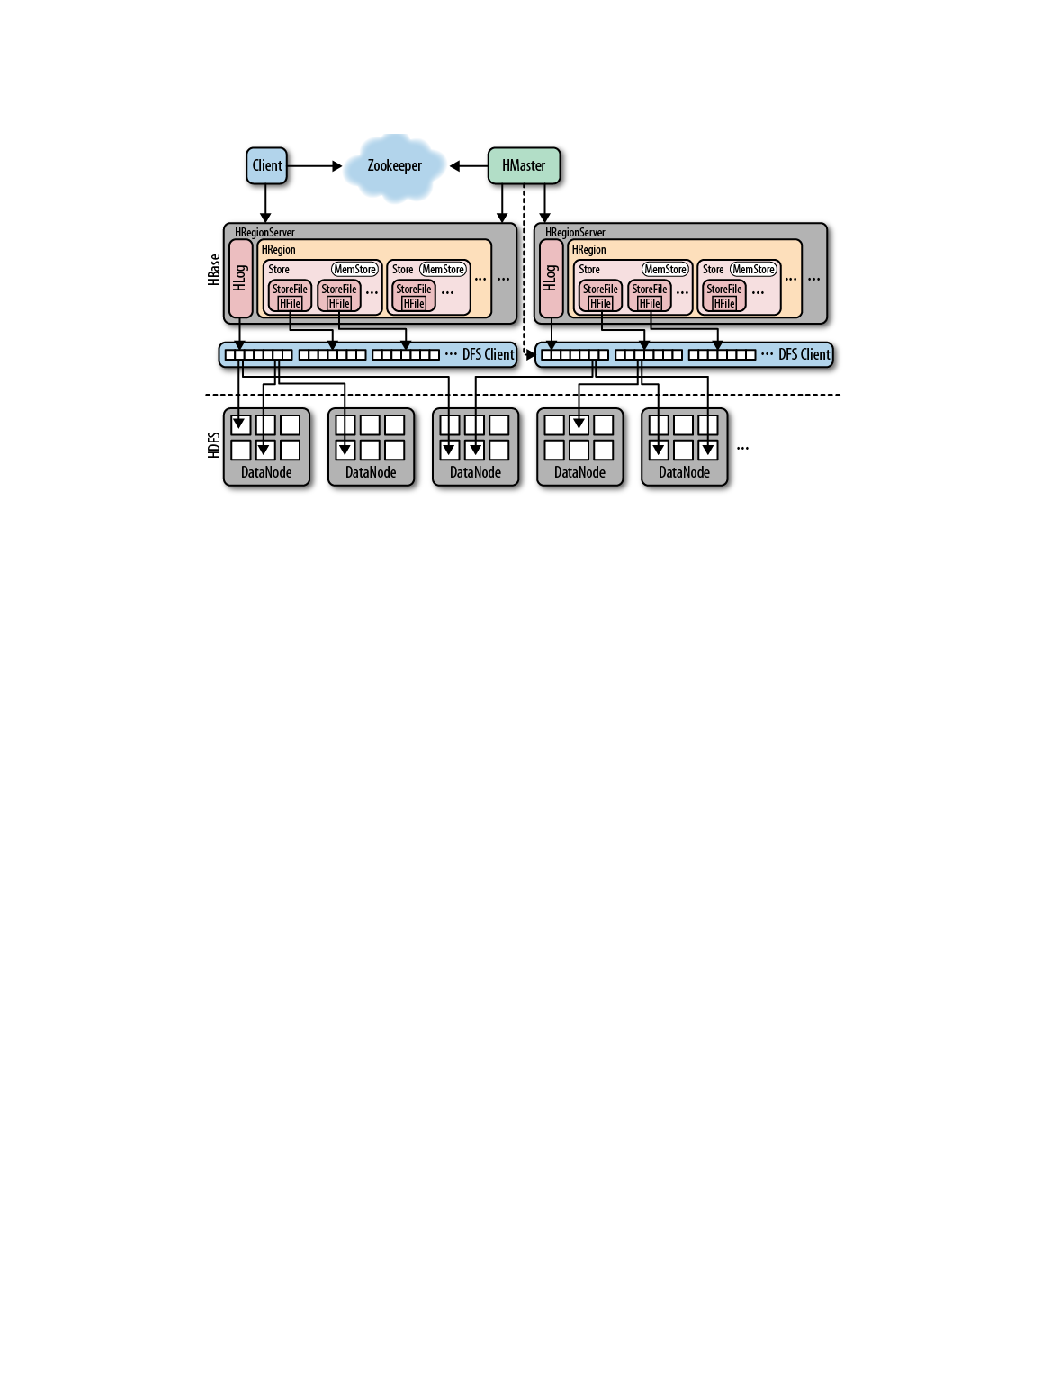
\includegraphics[scale=0.9]{./figures/hbase-storage}
    \caption{Overview of how HBase handles files in the filesystem}
    \label{fig:hbase-storage}
  \end{figure}
}

\frame {\frametitle{Storage}
  \begin{beamerboxesrounded}{}
    Overview
  \end{beamerboxesrounded}

  \begin{itemize}
  \item \textbf{HBase handles two kinds of file types}
    \begin{itemize}
    \item One is used for the WAL
    \item One is used for the actual data storage
    \end{itemize}

    \vspace{20pt}

  \item \textbf{Who does what}
    \begin{itemize}
    \item \texttt{HMaster}
      \begin{itemize}
      \item Low-level operations
      \item Assigns region servers to key space
      \item Keeps metadata
      \item Talks to ZooKeeper
      \end{itemize}
    \item \texttt{HRegionServer}
      \begin{itemize}
      \item Handles the WAL and \texttt{HFiles}
      \item These files are divided in to blocks and stored into HDFS
      \item Block size is a parameter
      \end{itemize}
    \end{itemize}

  \end{itemize}
}

\frame {\frametitle{Storage}
  \begin{beamerboxesrounded}{}
    Overview
  \end{beamerboxesrounded}

  \begin{itemize}
  \item \textbf{General communication flow}
    \begin{itemize}
    \item A client contacts ZooKeeper when trying to access a
      particular row
    \item Recovers from ZooKeeper the server name that host the
      \texttt{-ROOT-} region
    \item Using the \texttt{-ROOT-} information the client retrieves
      the server name that host the \texttt{.META.} table region
      \begin{itemize}
      \item The \texttt{.META.} table region contains the row key in question
      \end{itemize}
    \item Contact the reported \texttt{.META.} server and retrieve the
      server name that has the region containing the row key in question
    \end{itemize}

    \vspace{20pt}

  \item \textbf{Caching}
    \begin{itemize}
    \item Generally, lookup procedures involve caching row key
      locations for faster subsequent lookups
    \end{itemize}
  \end{itemize}
}

\frame {\frametitle{Storage}
  \begin{beamerboxesrounded}{}
    Overview
  \end{beamerboxesrounded}

  \begin{itemize}
  \item \textbf{Important Java Classes}
    \begin{itemize}
    \item \texttt{HRegionServer} handles one or more regions and
      create the corresponding \texttt{HRegion} object
    \item When an \texttt{HRegion} object is opened it creates
      a \texttt{Store} instance for each \texttt{HColumnFamily}
    \item Each \texttt{Store} instance can have:
      \begin{itemize}
      \item One or more \texttt{StoreFile} instances
      \item A \texttt{MemStore} instance
      \end{itemize}
    \item \texttt{HRegionServer} has a shared \texttt{HLog} instance
    \end{itemize}
  \end{itemize}
}

\frame {\frametitle{Storage}
  \begin{beamerboxesrounded}{}
    Write Path
  \end{beamerboxesrounded}

  \begin{itemize}
  \item \textbf{External client insert data in HBase}
    \begin{itemize}
    \item Issues an \texttt{HTable.put(Put)} request to \texttt{HRegionServer}
    \item \texttt{HRegionServer} hands the request to the \texttt{HRegion} instance that
      matches the request [{\color{red}Q: What is the matching criteria?}]
    \end{itemize}

    \vspace{20pt}

  \item \textbf{How the system reacts to a write request}
    \begin{itemize}
    \item Write data to the WAL, represented by the \texttt{HLog}
      class
      \begin{itemize}
      \item The WAL stores \texttt{HLogKey} instances in a HDFS
        \texttt{SequenceFile}
      \item These keys contain a sequence number and the actual data
      \item In case of failure, this data can be used to replay
        not-yet-persisted data
      \end{itemize}
    \item Copy data in the \texttt{MemStore}
      \begin{itemize}
      \item Check if MemStore size has reached a threshold
      \item If yes, launch a \textit{flush request}
      \item Launch a thread in the \texttt{HRegionServer} and flush \texttt{MemStore} data
        to an \texttt{HFile}
      \end{itemize}
    \end{itemize}
  \end{itemize}
}

\frame {\frametitle{Storage}
  \begin{beamerboxesrounded}{}
    HBase Files
  \end{beamerboxesrounded}

  \begin{itemize}
  \item \textbf{What and where are HBase files (including WAL,
    \texttt{HFile},...) stored?}
    \begin{itemize}
    \item HBase has a root directory set to ``\texttt{/hbase}'' in
      HDFS
    \item Files can be divided into:
      \begin{itemize}
      \item Those that reside under the HBase root directory
      \item Those that are in the \textit{per-table} directories
      \end{itemize}
    \end{itemize}

    \vspace{20pt}

  \item \texttt{/hbase}
    \begin{itemize}
    \item \texttt{.logs}
    \item \texttt{.oldlogs}
    \item \texttt{.hbase.id}
    \item \texttt{.hbase.version}
    \item \texttt{/example-table}
    \end{itemize}
  \end{itemize}
}

\frame {\frametitle{Storage}
  \begin{beamerboxesrounded}{}
    HBase Files
  \end{beamerboxesrounded}
  
  \begin{itemize}
  \item \texttt{/example-table}
    \begin{itemize}
    \item \texttt{.tableinfo}
    \item \texttt{.tmp}
    \item \texttt{``\texttt{...Key1...}''}
      \begin{itemize}
      \item \texttt{.oldlogs}
      \item \texttt{.regioninfo}
      \item \texttt{.tmp}
      \item \texttt{colfam1/}
      \end{itemize}
    \end{itemize}

  \item \texttt{colfam1/}
    \begin{itemize}
    \item ``\texttt{....column-key1...}''
    \end{itemize}
  \end{itemize}
}

\frame {\frametitle{Storage}
  \begin{beamerboxesrounded}{}
    HBase: Root-level files
  \end{beamerboxesrounded}

  \begin{itemize}
  \item \textbf{\texttt{.logs} directory}
    \begin{itemize}
    \item WAL files handled by \texttt{HLog} instances
    \item Contains a subdir for each \texttt{HRegionServer}
    \item Each subdir contains many \texttt{HLog} files
    \item All regions from that \texttt{HRegionServer} share the same
      HLog files
    \end{itemize}
  \item \texttt{.oldlogs} directory
    \begin{itemize}
    \item When data is persisted to disk (from \texttt{Memstores}) log
      files are decommissioned to the \texttt{.oldlogs} dir
    \end{itemize}

    \vspace{20pt}

  \item \textbf{\texttt{hbase.id} and \texttt{hbase.version}}
    \begin{itemize}
    \item Represent the unique ID of the cluster and the file format version
    \end{itemize}
  \end{itemize}
}

\frame {\frametitle{Storage}
  \begin{beamerboxesrounded}{}
    HBase: Table-level files
  \end{beamerboxesrounded}

  \begin{itemize}
  \item \textbf{Every table has its own directory}
    \begin{itemize}
    \item \texttt{.tableinfo}: stores the serialized
      \texttt{HTableDescriptor}
      \begin{itemize}
      \item This include the table and column family schema
      \end{itemize}
    \item \texttt{.tmp} directory
      \begin{itemize}
      \item Contains temporary data
      \end{itemize}
    \end{itemize}
  \end{itemize}
}

\frame {\frametitle{Storage}
  \begin{beamerboxesrounded}{}
    HBase: Region-level files
  \end{beamerboxesrounded}

  \begin{itemize}
  \item \textbf{Inside each table dir, there is a separate dir for every
      region in the table}
    \begin{itemize}
    \item The name of each of this dirs is the MD5 hash of a region name
      \begin{itemize}
      \item Inside each region there is a directory for each column
        family
      \item Each column family directory holds the actual data files,
        namely \texttt{HFiles}
      \item Their name is just an arbitrary random number
      \end{itemize}
    \item Each region directory also has a \texttt{.regioninfo} file
      \begin{itemize}
      \item Contains the serialized information of the \texttt{HRegionInfo} instance
      \end{itemize}
    \end{itemize}
    
    \vspace{20pt}
    
  \item \textbf{Split Files}
    \begin{itemize}
    \item Once the region needs to be split, a \texttt{splits}
      directory is created
      \begin{itemize}
      \item This is used to stage two daughter regions
      \item If split is successful, daughter regions are moved up to
        the table directory
      \end{itemize}
    \end{itemize}
  \end{itemize}
}

\frame {\frametitle{Storage}
  \begin{beamerboxesrounded}{}
    HBase: A note on region splits
  \end{beamerboxesrounded}

  \begin{itemize}
  \item \textbf{Splits triggered by store file (region) size}
    \begin{itemize}
    \item Region is split in two
    \item Region is closed to new requests
    \item \texttt{.META.} is updated
    \end{itemize}
    
    \vspace{20pt}
    
  \item \textbf{Daughter regions initially reside on the same server}
    \begin{itemize}
    \item Both daughters are compacted
    \item Parent is cleaned up
    \item \texttt{.META.} is updated
    \end{itemize}
    
    \vspace{20pt}
    
  \item \textbf{Master schedules new regions to be moved off to other servers}
  \end{itemize}  
}

\frame {\frametitle{Storage}
  \begin{beamerboxesrounded}{}
    HBase: Compaction
  \end{beamerboxesrounded}

  \begin{itemize}
  \item \textbf{Process that takes care of re-organizing store files}
    \begin{itemize}
    \item Essentially to conform to underlying filesystem requirements
    \item Compaction check when memstore is flushed
    \end{itemize}

    \vspace{20pt}

  \item \textbf{Minor and Major compactions}
    \begin{itemize}
    \item Always from the oldest to the newest files
    \item Avoid all servers to perform compaction concurrently
    \end{itemize}
  \end{itemize}

  \begin{figure}[h]
    \centering
    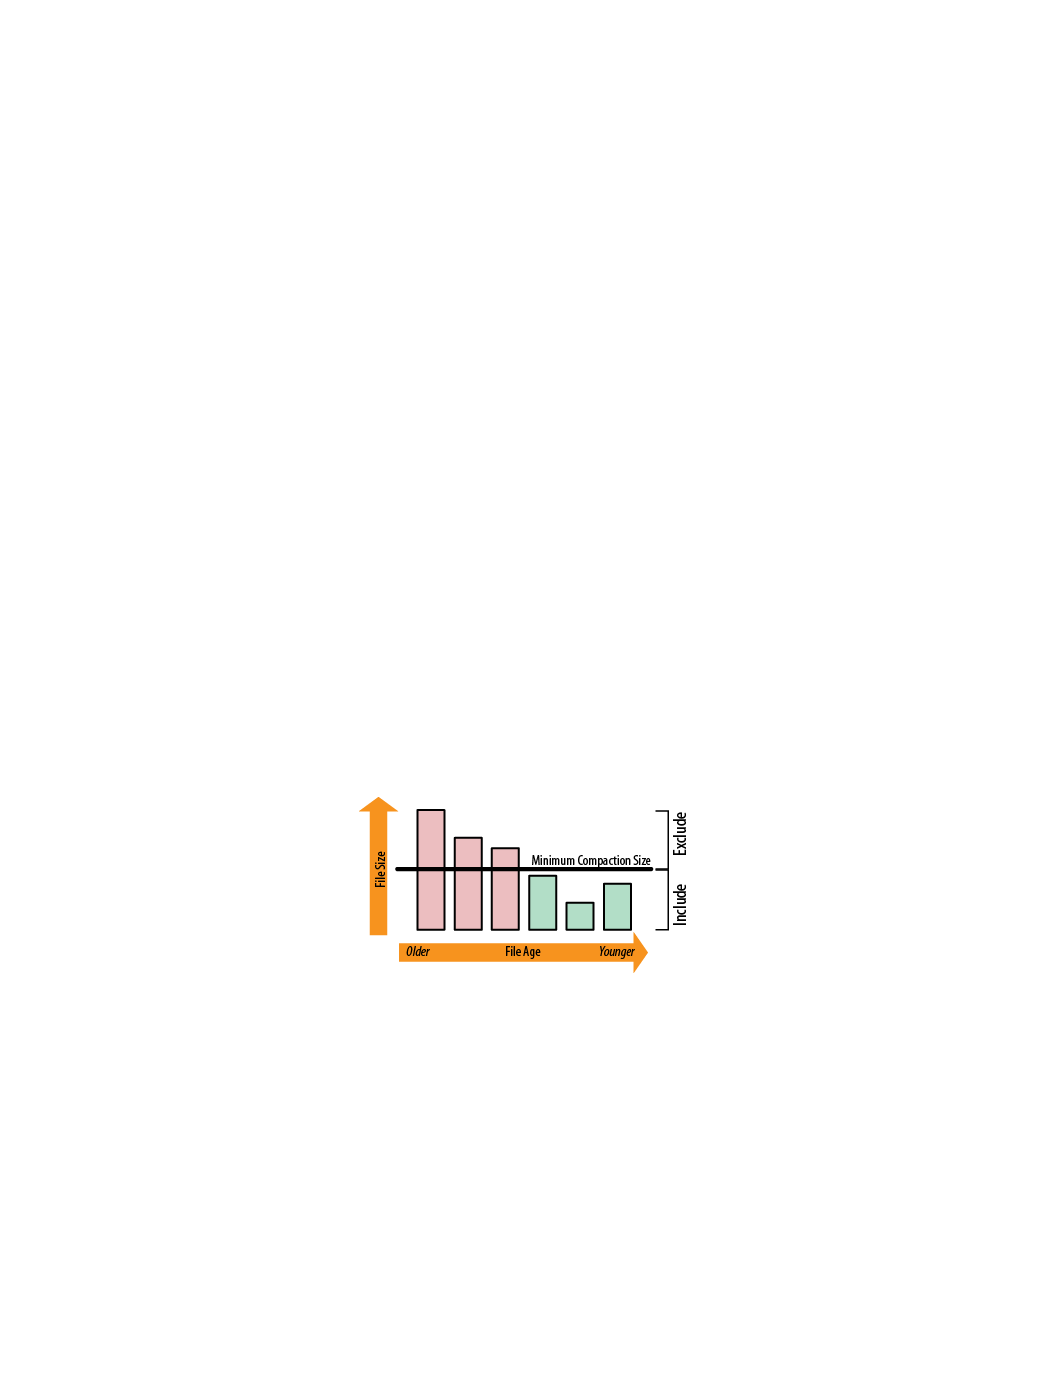
\includegraphics[scale=0.7]{./figures/compaction}
    \caption{A set of store files showing the minimum compaction threshold}
    \label{fig:compaction}
  \end{figure}
}

\frame {\frametitle{Storage}
  \begin{beamerboxesrounded}{}
    HFile format
  \end{beamerboxesrounded}

  \begin{itemize}
  \item \textbf{Store files are implemented by the \texttt{HFile} class}
    \begin{itemize}
    \item Efficient data storage is the goal
    \end{itemize}

    \vspace{20pt}

  \item \textbf{\texttt{HFiles} consist of a variable number of
      blocks}
    \begin{itemize}
    \item Two fixed blocks: \textit{info} and \textit{trailer}
    \item \textit{index} block: records the offsets of the \texttt{data} and
      meta \texttt{blocks}
    \item Block size: \textit{large} $\to$ sequential access; \textit{small} $\to$
      random access
    \end{itemize}
  \end{itemize}

  \begin{figure}[h]
    \centering
    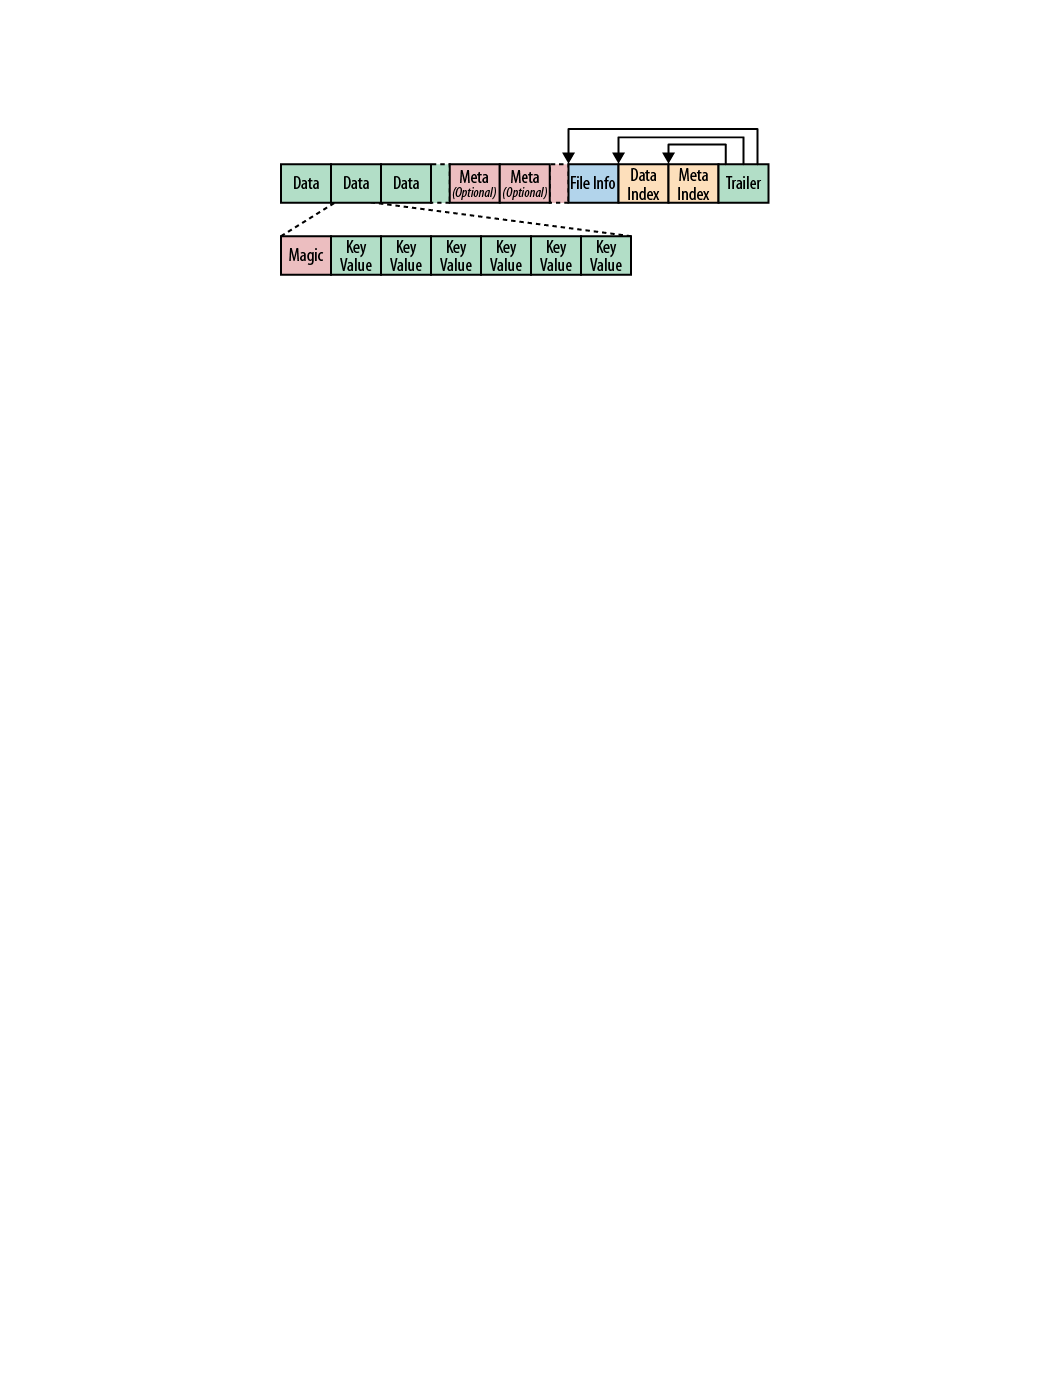
\includegraphics[scale=0.8]{./figures/hfile}
    \caption{The HFile structure}
    \label{fig:hfile}
  \end{figure}
}

\frame {\frametitle{Storage}
  \begin{beamerboxesrounded}{}
    HFile size and HDFS block size
  \end{beamerboxesrounded}

  \begin{itemize}
  \item \textbf{HBase uses any underlying filesystem}

    \vspace{20pt}

  \item \textbf{In case HDFS is used}
    \begin{itemize}
    \item HDFS block size is generally 64MB
    \item This is 1,024 times the default \texttt{HFile} block size
      (64 KB)
    \item[$\to$] There is no correlation between HDFS block and HFile sizes
    \end{itemize}
  \end{itemize}
}

\frame {\frametitle{Storage}
  \begin{beamerboxesrounded}{}
    The KeyValue Format
  \end{beamerboxesrounded}

  \begin{itemize}
  \item \textbf{Each KeyValue in the HFile is a low-level byte array}
    \begin{itemize}
    \item It allows for \textit{zero-copy} access to the data
    \end{itemize}

    \vspace{20pt}

  \item \textbf{Format}
    \begin{itemize}
    \item Fixed-length preambule indicates the length of the key and
      value
      \begin{itemize}
      \item This is useful to offset into the array to get direct
        access to the value, ignoring the key
      \end{itemize}
    \item Key format
      \begin{itemize}
      \item Contains row key, column family name, column qualifier...
      \item \texttt{[TIP]}: consider small keys to avoid overhead when storing
        small data
      \end{itemize}
    \end{itemize}
  \end{itemize}

  \begin{figure}[h]
    \centering
    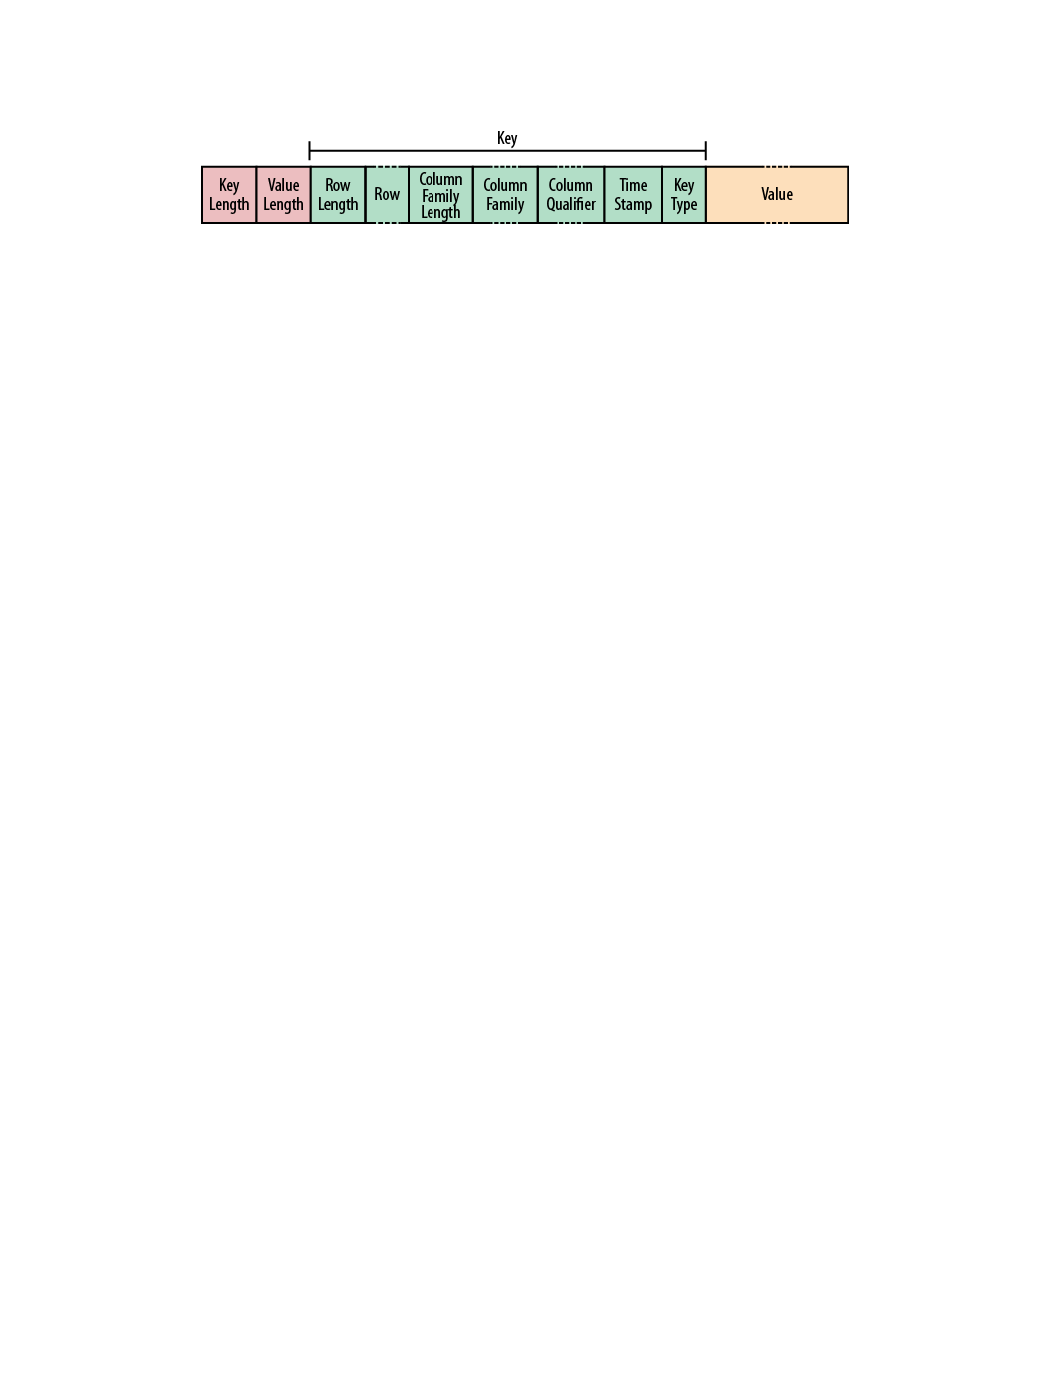
\includegraphics[scale=0.8]{./figures/keyvalue}
    \caption{The KeyValue Format}
    \label{fig:keyvalue}
  \end{figure}


}

%%%%%%%%%%%%%%%%%%%%%%%%%%%%%%%%%%%%%%%%%%%%%%%%%%%%%%%%%%
\subsection{WAL}
%%%%%%%%%%%%%%%%%%%%%%%%%%%%%%%%%%%%%%%%%%%%%%%%%%%%%%%%%%
\frame {\frametitle{The Write-Ahead Log}

  \begin{itemize}
  \item \textbf{Main tool to ensure resiliency to failures}
    \begin{itemize}
    \item Region servers keep data in-memory until enough is collected
      to warrant a flush
    \item What if the server crashes or power is lost?
    \end{itemize}

    \vspace{20pt}

  \item \textbf{WAL is a common approach to address fault-tolerance}
    \begin{itemize}
    \item Every data update is first written to a log
    \item Log is persisted (and replicated, since it resides on HDFS)
    \item Only when log is written, client is notified a successful
      operation on data
    \end{itemize}
  \end{itemize}

}

\frame {\frametitle{The Write-Ahead Log}

  \begin{figure}[h]
    \centering
    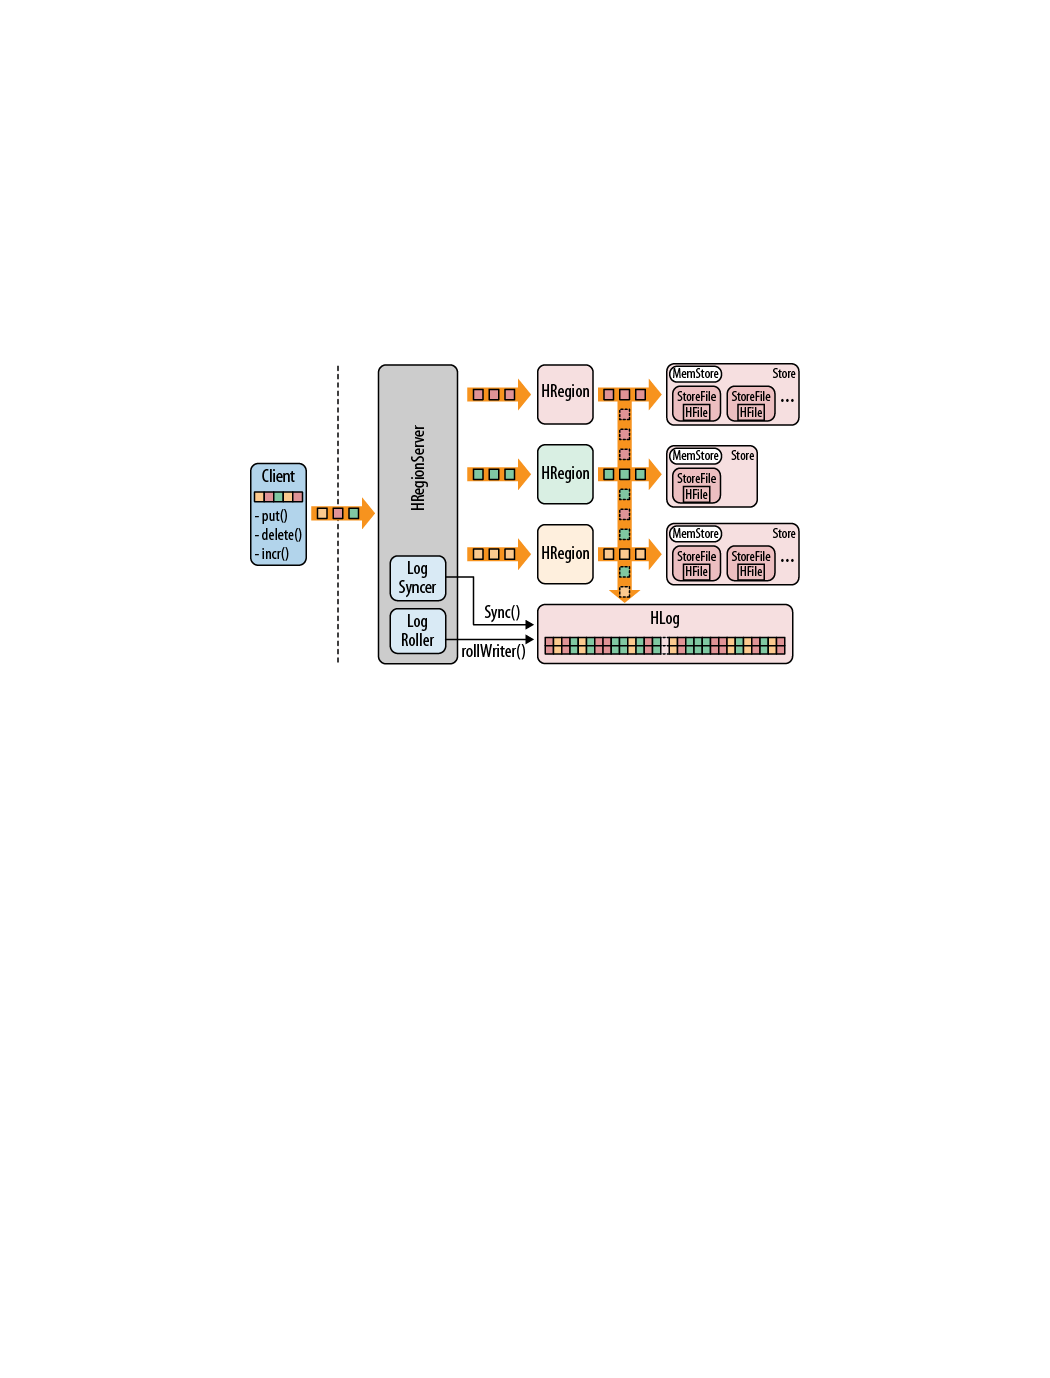
\includegraphics[scale=0.8]{./figures/wal}
    \caption{The write path of HBase}
    \label{fig:wal}
  \end{figure}

  \begin{itemize}
  \item \textbf{WAL records all changes to data}
    \begin{itemize}
    \item Can be replayed in case of server failure
    \item If write to WAL fails, the whole operations has to fail
    \end{itemize}
  \end{itemize}
}

\frame {\frametitle{The Write-Ahead Log}

  \begin{figure}[h]
    \centering
    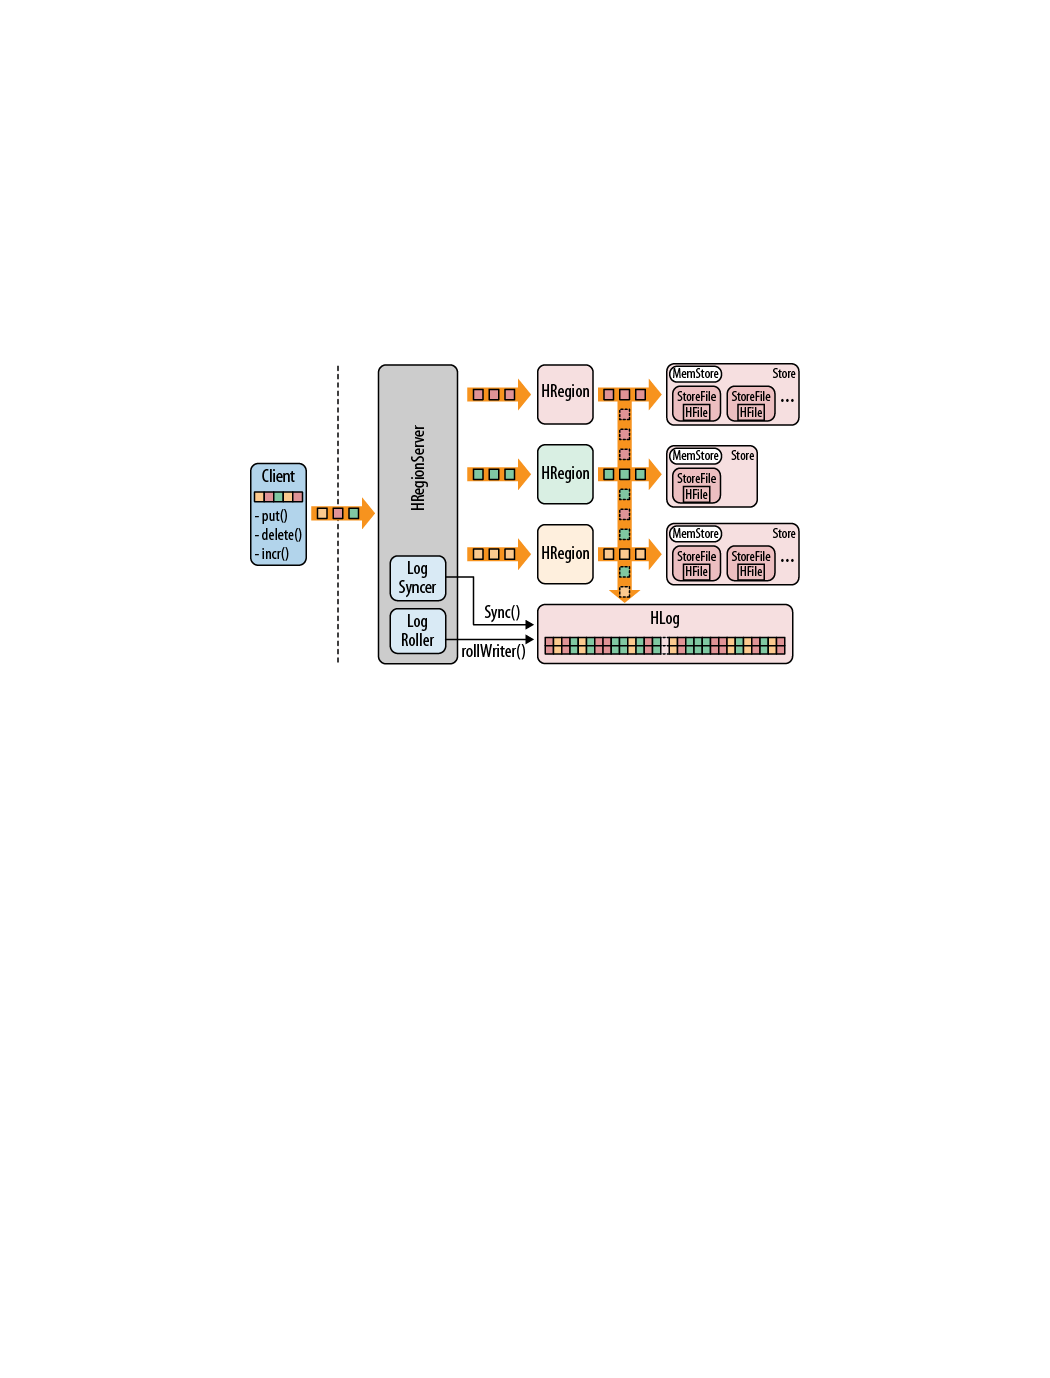
\includegraphics[scale=0.8]{./figures/wal}
  \end{figure}

  \begin{itemize}
  \item \textbf{Write Path}
    \begin{itemize}
    \item Client modifies data (\texttt{put()}, \texttt{delete()},
      \texttt{increment()})
    \item Modifications are wrapped into a KeyValue object
    \item Objects are batched to the corresponding
      \texttt{HRegionServer}
    \item Objects are routed to the corresponding \texttt{HRegion}
    \item Objects are written to WAL and in the \texttt{MemStore}
    \end{itemize}
  \end{itemize}
}


%%%%%%%%%%%%%%%%%%%%%%%%%%%%%%%%%%%%%%%%%%%%%%%%%%%%%%%%%%
\subsection{Read Path}
%%%%%%%%%%%%%%%%%%%%%%%%%%%%%%%%%%%%%%%%%%%%%%%%%%%%%%%%%%
\frame {\frametitle{Read Path}
  \begin{itemize}
  \item \textbf{HBase uses multiple store files per column family}
    \begin{itemize}
    \item These can be either in-memory and/or materialized on disk
    \item Compactions and clean-up background processes take care of
      store files maintenance
    \item Store files are immutable, so deletion is handled in a
      special way
    \end{itemize}

    \vspace{20pt}

  \item \textbf{The anatomy of a \texttt{get} command}
    \begin{itemize}
    \item HBase uses a \texttt{QueryMatcher} in combination with a
      \texttt{ColumnTracker}
    \item First, an exclusion check is performed to filter skip files
      (and eventually tombstone labelled data)
    \item Scanning data is implemented by a \texttt{RegionScanner}
      class which retrieves a \texttt{StoreScanner}
    \item \texttt{StoreScanner} includes both the \texttt{MemStore}
      and \texttt{HFiles}
    \item Read/Scans happen in the same order as data is saved
    \end{itemize}
  \end{itemize}
}

%%%%%%%%%%%%%%%%%%%%%%%%%%%%%%%%%%%%%%%%%%%%%%%%%%%%%%%%%%
\subsection{Region Lookups}
%%%%%%%%%%%%%%%%%%%%%%%%%%%%%%%%%%%%%%%%%%%%%%%%%%%%%%%%%%
\frame {\frametitle{Region Lookups}
  \begin{itemize}
  \item \textbf{How does a client find the region server hosting a specific
      row key range?}
    \begin{itemize}
    \item HBase uses two special catalog tables, \texttt{-ROOT-} and
      \texttt{.META.}
    \item The \texttt{-ROOT-} table is used to refer to all regions in the
      \texttt{.META.} table
    \end{itemize}
    
    \vspace{20pt}
    
  \item \textbf{Three-level B+ Tree -like operation}
    \begin{itemize}
    \item Level 1: a node stored in ZooKeeper, containing the location
      (region server) of the \texttt{-ROOT-} table
    \item Level 2: Lookup in the -ROOT- table to find a matching meta
      region
    \item Level 3: Retrieve the table region from the \texttt{.META.} table
    \end{itemize}
  \end{itemize}
}

\frame {\frametitle{Region Lookups}
  \begin{itemize}
  \item \textbf{Where to send requests when looking for a specific row
      key?}
    \begin{itemize}
    \item This information is cached, but the first time or when the
      cache is stale or when there is a miss due to compaction, the
      following procedure applies
    \end{itemize}

    \vspace{20pt}

  \item \textbf{Recursive discovery process}
    \begin{itemize}
    \item Ask the region server hosting the matching \texttt{.META.}
      table to retrieve the row key address
    \item If the information is invalid, it backs out: asks the
      \texttt{-ROOT-} table where the relevant \texttt{.META.} region
      is
    \item If this fails, ask ZooKeeper where the \texttt{-ROOT-} table is
    \end{itemize}
  \end{itemize}
}

\frame {\frametitle{Region Lookups}
  \begin{figure}[h]
    \centering
    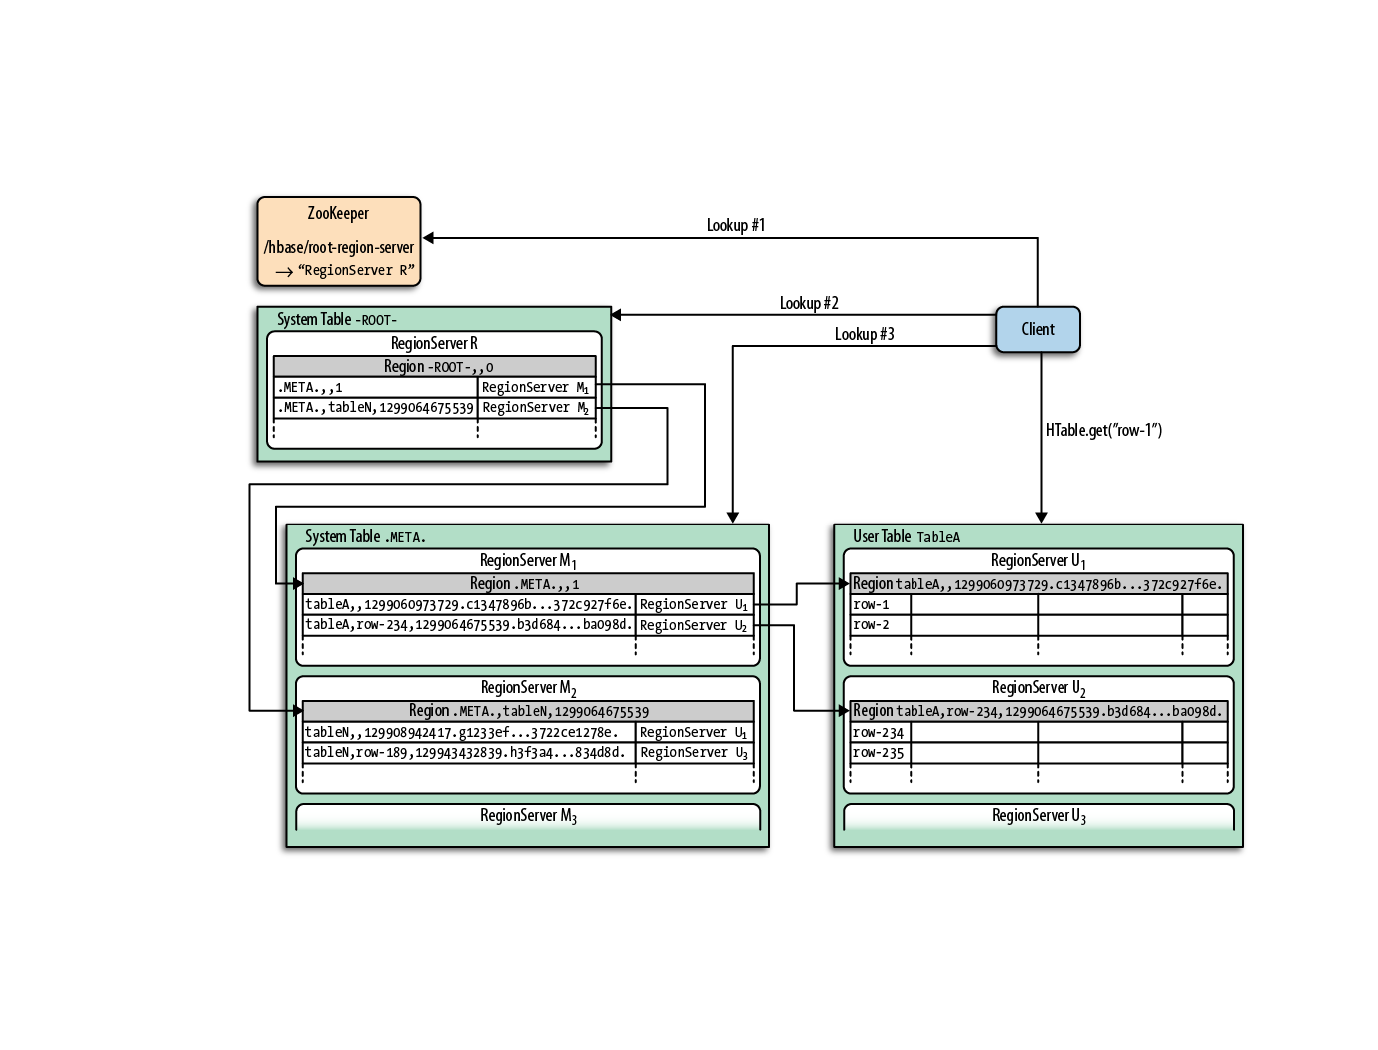
\includegraphics[scale=0.6]{./figures/lookup}
  \end{figure}
}
\subsection{Key Design}
%%%%%%%%%%%%%%%%%%%%%%%%%%%%%%%%%%%%%%%%%%%%%%%%%%%%%%%%%%
\begin{frame}
  \begin{beamerboxesrounded}{}
	\begin{center}

\vspace{20pt}

		Key Design

\vspace{20pt}

	\end{center}    
  \end{beamerboxesrounded}
\end{frame}


%%%%%%%%%%%%%%%%%%%%%%%%%%%%%%%%%%%%%%%%%%%%%%%%%%%%%%%%%%
\subsection{Concepts}
%%%%%%%%%%%%%%%%%%%%%%%%%%%%%%%%%%%%%%%%%%%%%%%%%%%%%%%%%%
\frame {\frametitle{Concepts}
  \begin{itemize}
  \item \textbf{HBase has two fundamental key structures}
    \begin{itemize}
    \item Row key
    \item Column key
    \end{itemize}

    \vspace{20pt}

  \item \textbf{Both can be used to convey meaning}
    \begin{itemize}
    \item Because they store particularly meaningful data
    \item Because their sorting order is important
    \end{itemize}
  \end{itemize}
}

\frame {\frametitle{Concepts}
  \begin{itemize}
  \item \textbf{Logical vs. on-disk layout of a table}
    \begin{itemize}
    \item Main unit of separation within a table is the \textit{column
        family}
    \item The actual columns (as opposed to other column-oriented DB)
      are not used to separate data
    \item Although cells are stored logically in a table format, rows
      are stored as linear sets of the cells
    \item Cells contain all the vital information inside them
    \end{itemize}
  \end{itemize}

  \begin{figure}[h]
    \centering
    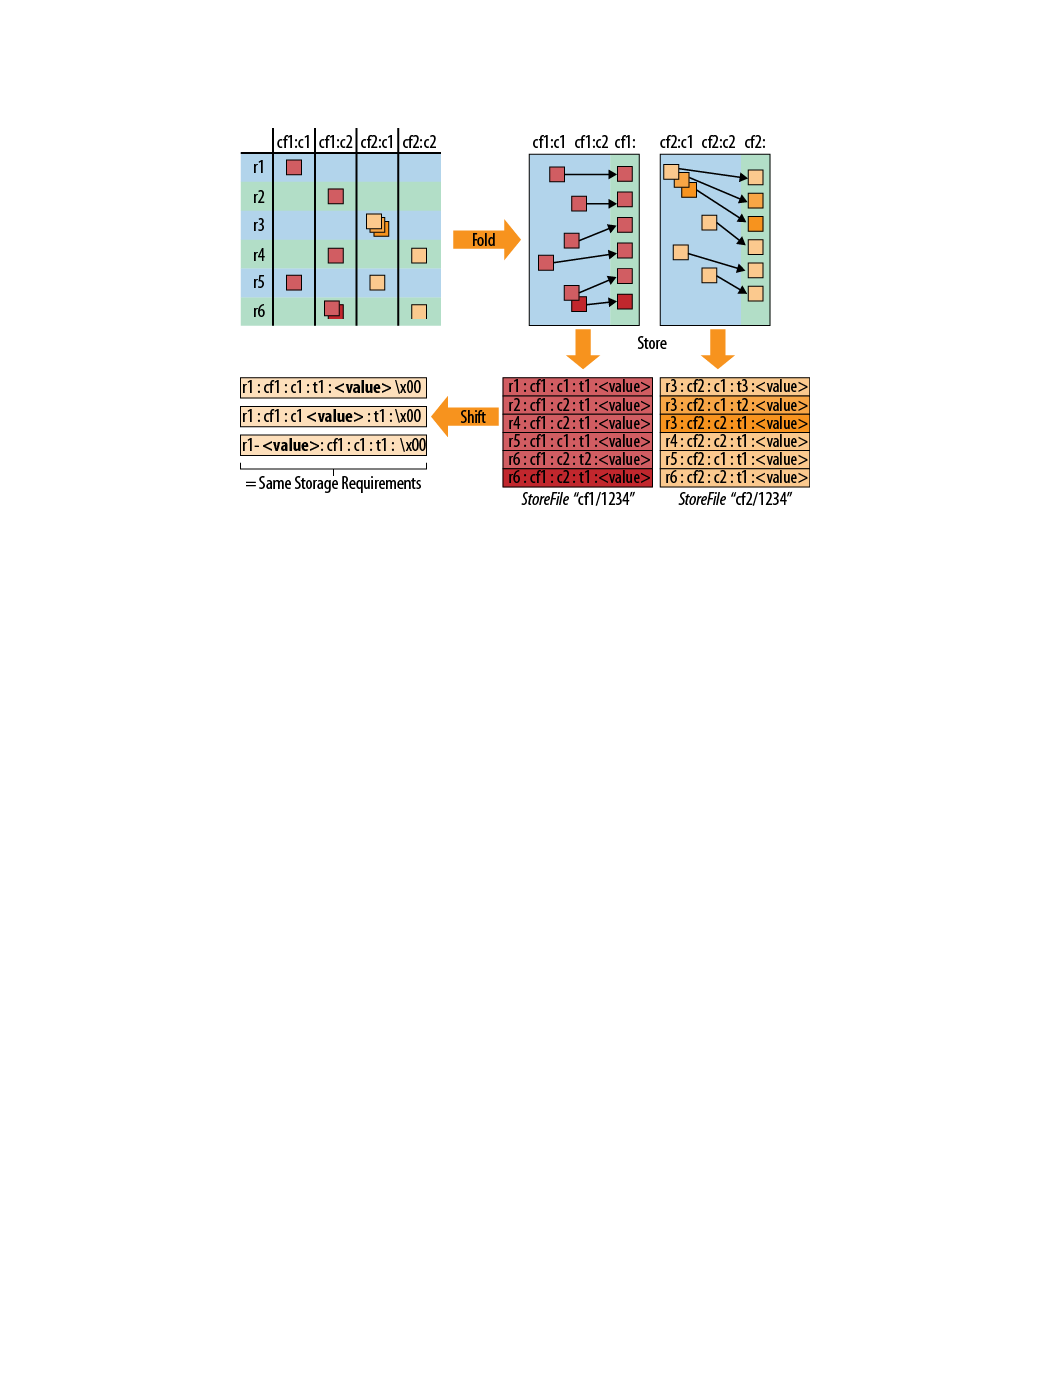
\includegraphics[scale=0.7]{./figures/layout}
  \end{figure}
}

\frame {\frametitle{Concepts}
  \begin{figure}[h]
    \centering
    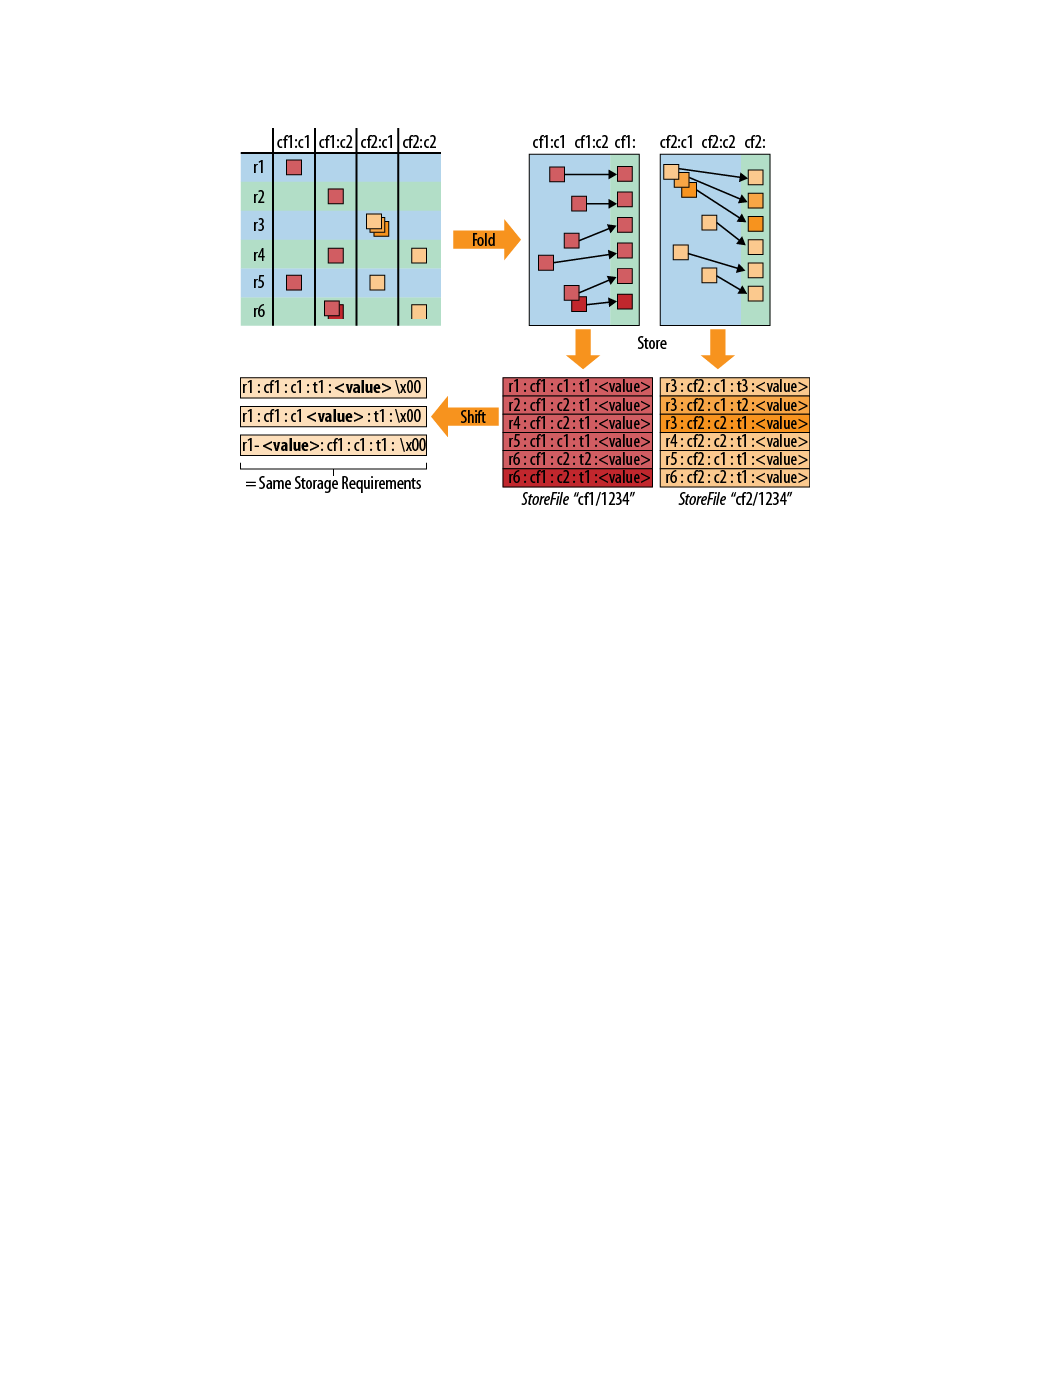
\includegraphics[scale=0.7]{./figures/layout}
  \end{figure}

  \begin{itemize}
  \item \textbf{Logical Layout (Top-Left)}
    \begin{itemize}
    \item Table consists of rows and columns
    \item Columns are the combination of a column family name and a
      column qualifier
    \item[$\to$] \texttt{<cf name: qualifier>} is the \textbf{column
        key}
    \item Rows have a \textbf{row key} to address all columns of a
      single logical row
    \end{itemize}
  \end{itemize}
}

\frame {\frametitle{Concepts}
  \begin{figure}[h]
    \centering
    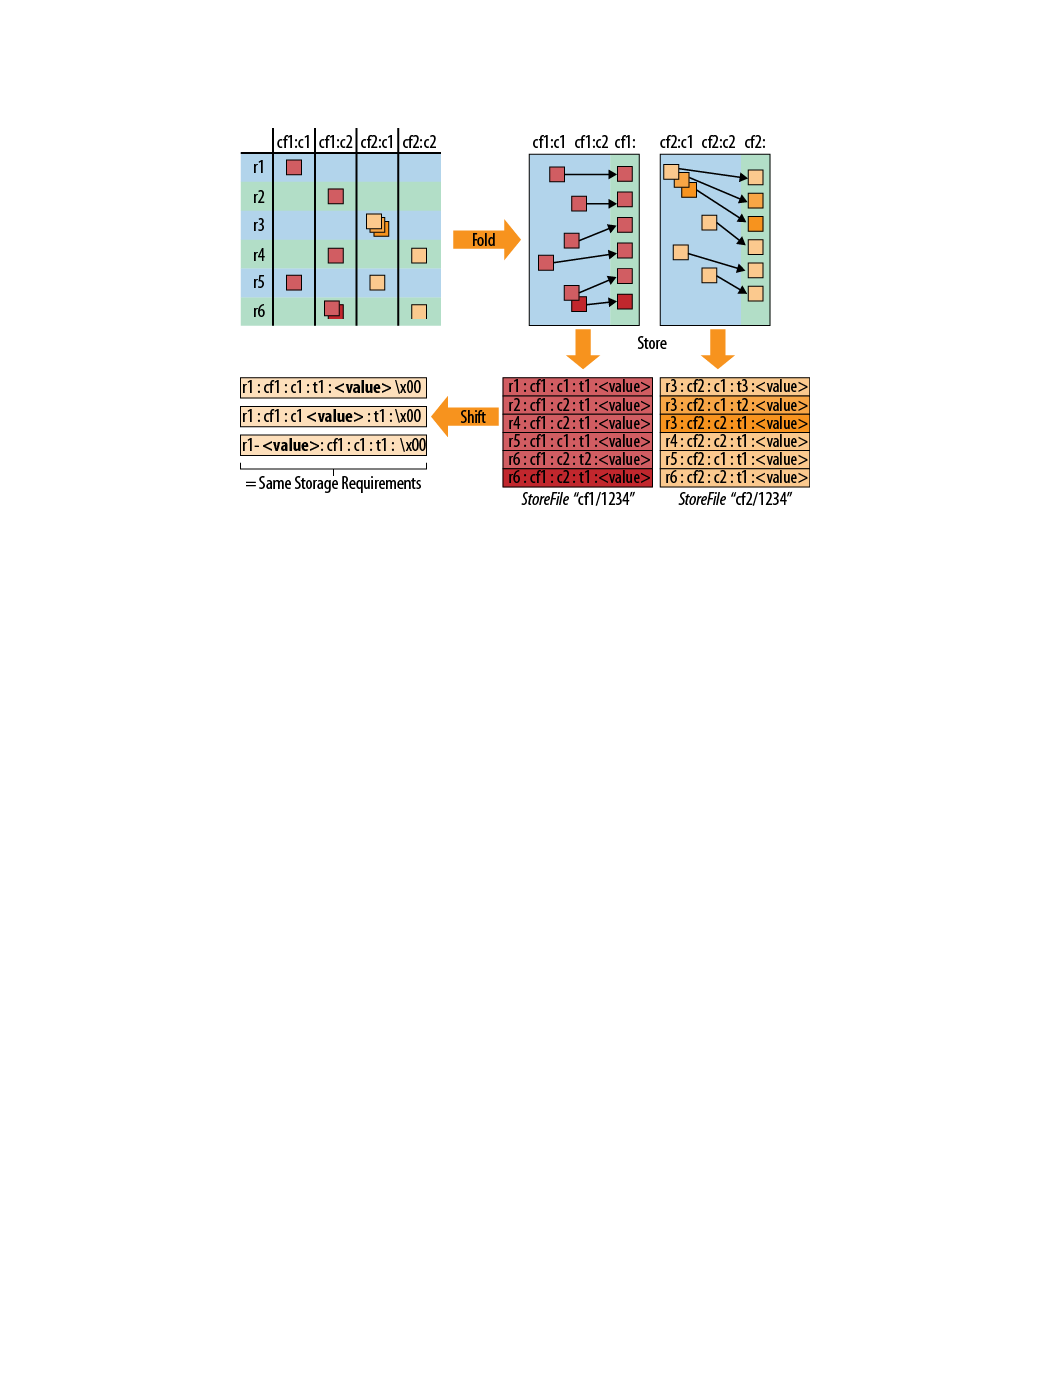
\includegraphics[scale=0.7]{./figures/layout}
  \end{figure}

  \begin{itemize}
  \item \textbf{Folding the Logical Layout (Top-Right)}
    \begin{itemize}
    \item The cells of each row are stored one after the other
    \item Each column family are stored separately
    \item[$\to$] On disk all cells of one family reside on an
      individual \texttt{StoreFile}
    \item HBase does not store unset cells
    \item[$\to$] \textbf{Row and column key is required to address every cell}
    \end{itemize}
  \end{itemize}
}

\frame {\frametitle{Concepts}
  \begin{itemize}
  \item \textbf{Versioning}
    \begin{itemize}
    \item Multiple versions of the same cell stored
      consecutively, together with the \textit{timestamp}
    \item Cells are sorted in descending order of timestamp
    \item[$\to$] Newest value first
    \end{itemize}

    \vspace{20pt}

  \item \textbf{\texttt{KeyValue} object}
    \begin{itemize}
    \item The entire cell, with all the structural information, is a
      \texttt{KeyValue} object
    \item Contains: \texttt{row key}, \texttt{<column family:
        qualifier>} $\to$ \texttt{column key}, \texttt{timestamp} and
      \texttt{value}
    \item Sorted by row key first, then by column key
    \end{itemize}

  \end{itemize}
}

\frame {\frametitle{Concepts}
  \begin{figure}[h]
    \centering
    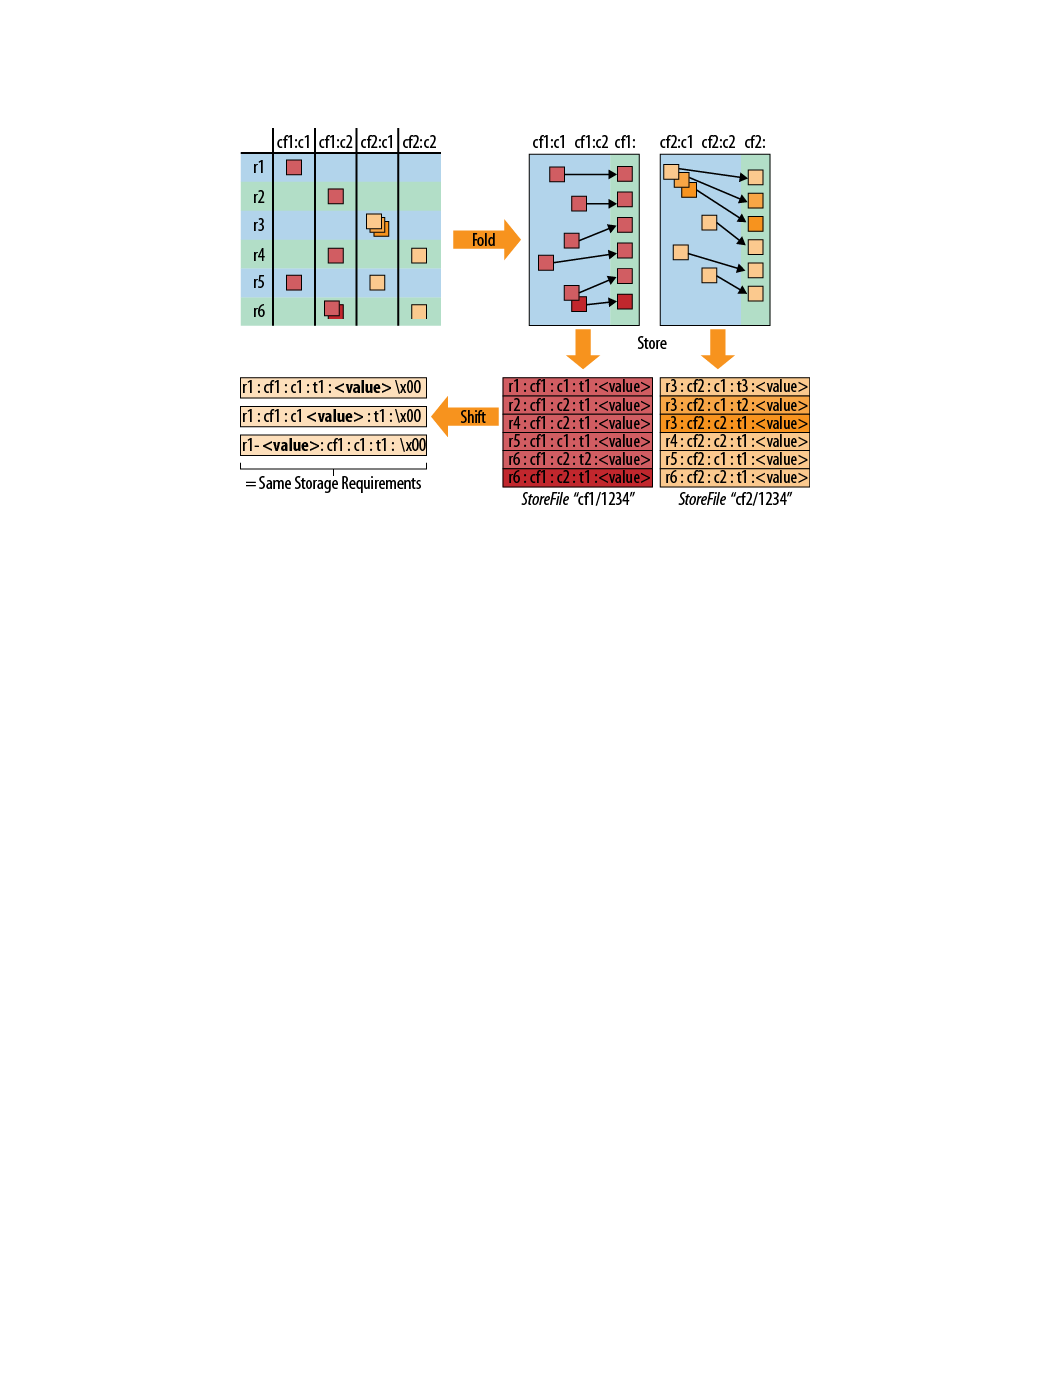
\includegraphics[scale=0.7]{./figures/layout}
  \end{figure}

  \begin{itemize}
  \item \textbf{Physical Layout (Lower-Right)}
    \begin{itemize}
    \item Select data by row key
      \begin{itemize}
      \item This reduces the amount of data to scan for a row or a
        range of rows
      \end{itemize}
    \item Select data by row key and column key
      \begin{itemize}
      \item This focuses the system on an individual storage file
      \end{itemize}
    \item Select data by column qualifier
      \begin{itemize}
      \item Exact lookups, including filters to omit useless data
      \end{itemize}
    \end{itemize}
  \end{itemize}
}

\frame {\frametitle{Concepts}
  \begin{itemize}
  \item \textbf{Summary of key lookup properties}
  \end{itemize}

\vspace{20pt}

 \begin{figure}[h]
    \centering
    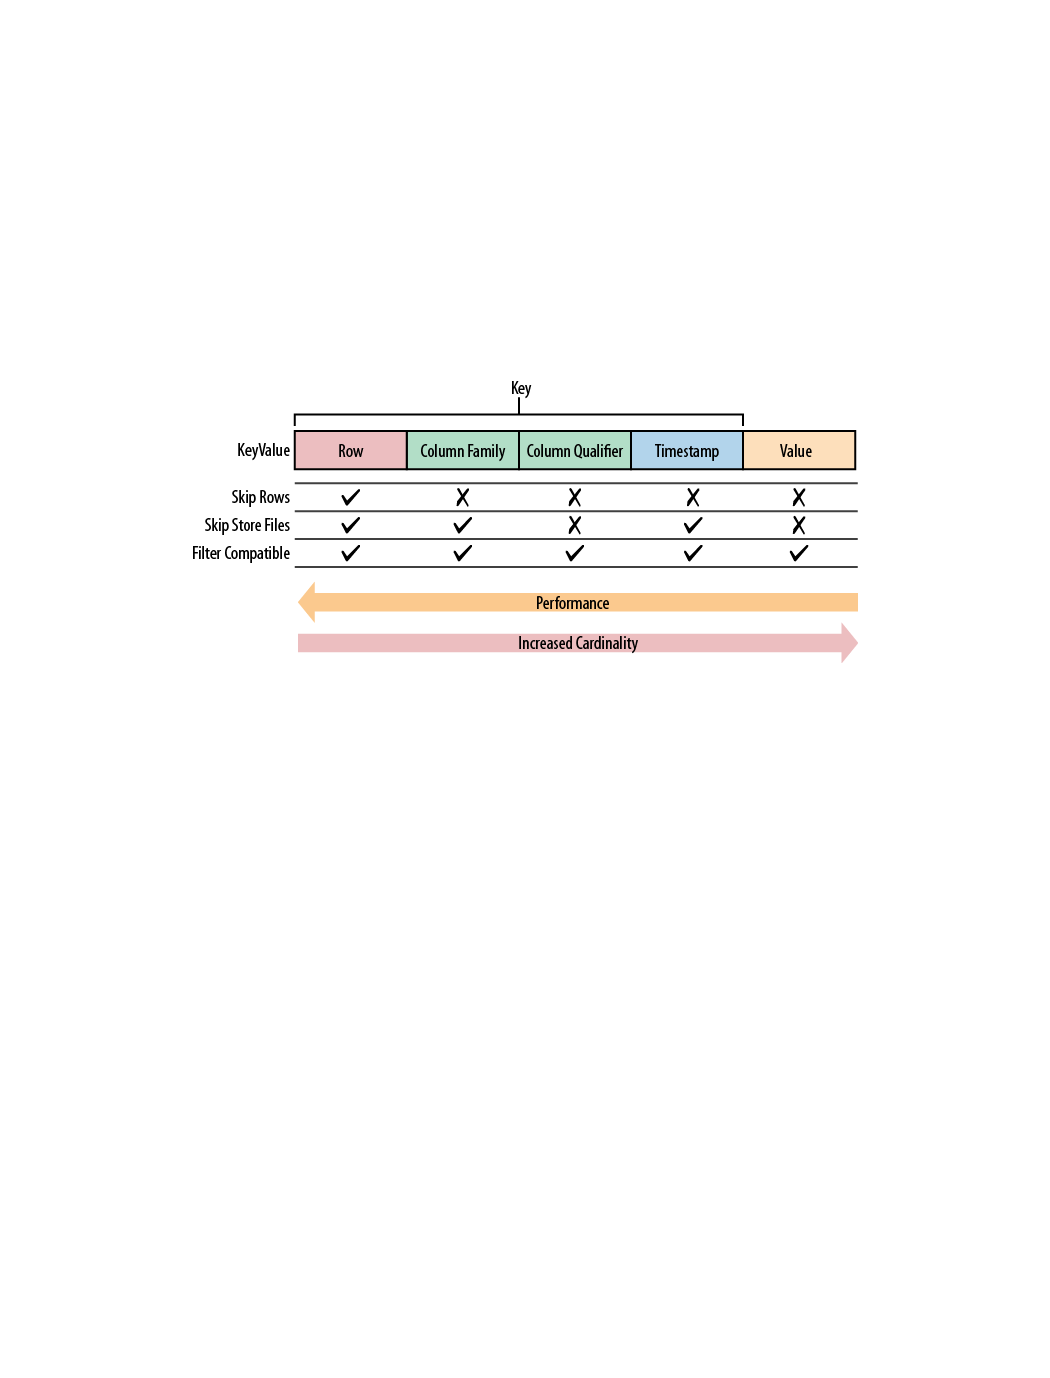
\includegraphics[scale=0.8]{./figures/key-lookup}
  \end{figure}

}

%%%%%%%%%%%%%%%%%%%%%%%%%%%%%%%%%%%%%%%%%%%%%%%%%%%%%%%%%%
\subsection{Tall-Narrow vs. Flat-Wide}
%%%%%%%%%%%%%%%%%%%%%%%%%%%%%%%%%%%%%%%%%%%%%%%%%%%%%%%%%%
\frame {\frametitle{Tall-Narrow vs. Flat-Wide Tables}
  \begin{itemize}
  \item \textbf{Tall-Narrow Tables}
    \begin{itemize}
    \item Few columns
    \item Many rows
    \end{itemize}

    \vspace{20pt}

  \item \textbf{Flat-Wide Tables}
    \begin{itemize}
    \item Many columns
    \item Few rows
    \end{itemize}

    \vspace{20pt}

  \item \textbf{Given the query granularity explained before}
    \begin{itemize}
    \item[$\to$] Store parts of the cell data in the row key
    \item Furthermore, HBase splits at row boundaries
    \item[$\to$] It is recommended to go for Tall-Narrow Tables
    \end{itemize}

  \end{itemize}
}

\frame {\frametitle{Tall-Narrow vs. Flat-Wide Tables}
  \begin{itemize}
  \item \textbf{Example: email data - version 1}
    \begin{itemize}
    \item You have all emails of a user in a single row (e.g. \texttt{userID}
      is the row key)
    \item There will be some outliers with orders of magnitude more
      emails than others
    \item[$\to$] A single row could outgrow the maximum file/region
      size and work against split facility
    \end{itemize}

    \vspace{20pt}

  \item \textbf{Example: email data - version 2}
    \begin{itemize}
    \item Each email of a user is stored in a separate row
      (e.g. \texttt{userID:messageID} is the row key)
    \item On disk this makes no difference (see the disk layout
      figure)
      \begin{itemize}
      \item If the \texttt{messageID} is in the column qualifier or
        the row key, each cell still contains a single email message
      \end{itemize}
    \item[$\to$] The table can be split easily and the query
      granularity is more fine-grained
    \end{itemize}

  \end{itemize}

}


%%%%%%%%%%%%%%%%%%%%%%%%%%%%%%%%%%%%%%%%%%%%%%%%%%%%%%%%%%
\subsection{Partial Key Scans}
%%%%%%%%%%%%%%%%%%%%%%%%%%%%%%%%%%%%%%%%%%%%%%%%%%%%%%%%%%
\frame {\frametitle{Partial Key Scans}
  \begin{itemize}
  \item \textbf{Partial Key Scans reinforce the concept of Tall-Narrow Tables}
    \begin{itemize}
    \item From the email example: assume you have a separate row per
      message, across all users
    \item If you don't have an exact combination of user and message
      ID you cannot access a particular message
    \end{itemize}

    \vspace{20pt}

  \item \textbf{Partial Key Scan solves the problems}
    \begin{itemize}
    \item Specify a \textit{start} and \textit{end} key
    \item The start key is set to the exact \texttt{userID} only, with the
      end key set at \texttt{userID+1}
    \item[$\to$] This triggers the internal lexicographic comparison
      mechanism
      \begin{itemize}
      \item Since the table does not have an exact match, it positions
        the scan at: \texttt{<userID>:<lowest-messageID>}
      \end{itemize}
    \item The scan will then iterate over all the messages of an exact
      user, parse the row key and get the \texttt{messageID}
    \end{itemize}

  \end{itemize}
}

\frame {\frametitle{Partial Key Scans}
  \begin{itemize}
  \item \textbf{Composite keys and atomicity}
    \begin{itemize}
    \item Following the email example: a single user inbox now spans
      many rows
    \item It is no longer possible to modify a single user inbox in
      one atomic operation
    \end{itemize}

    \vspace{20pt}

  \item \textbf{If this is acceptable or not, depends on the application at hand}

  \end{itemize}
}

%%%%%%%%%%%%%%%%%%%%%%%%%%%%%%%%%%%%%%%%%%%%%%%%%%%%%%%%%%
\subsection{Time Series Data}
%%%%%%%%%%%%%%%%%%%%%%%%%%%%%%%%%%%%%%%%%%%%%%%%%%%%%%%%%%
\frame {\frametitle{Time Series Data}
  \begin{itemize}
  \item \textbf{Stream processing of events}
    \begin{itemize}
    \item E.g. data coming from a sensor, stock exchange, monitoring
      system ...
    \item Such data is a time series $\to$ \textbf{The row key represents the
      event time}
  \item[$\to$] HBase will store all rows sorted in a distinct range,
    namely regions with specific start and stop keys
    \end{itemize}

    \vspace{20pt}

  \item \textbf{Sequential monotonously increasing nature of time
      series data}
    \begin{itemize}
    \item All incoming data is written to the same region (and hence
      the same server)
    \item[$\to$] \textbf{Regions become HOT!}
    \item Performance of the whole cluster is bound to that of a
      single machine
    \end{itemize}
  \end{itemize}
}

\frame {\frametitle{Time Series Data}
  \begin{itemize}
  \item \textbf{Solution to achieve load balancing: Salting}
    \begin{itemize}
    \item We want data to be spread over all region servers
    \item This can be done, e.g., by prefixing the row key with a
      non-sequential number
    \end{itemize}
  \end{itemize}
  
  \vspace{10pt}
  
  \begin{beamerboxesrounded}{\textbf{Salting example}}
    
    \begin{footnotesize}
      \texttt{byte prefix = (byte) (Long.hashCode(timestamp) \% <number of region servers>);\\
        byte[] rowkey = Bytes.add(Bytes.toBytes(prefix),
        Bytes.toBytes(timestamp));}
    \end{footnotesize} 
  \end{beamerboxesrounded}

  \vspace{10pt}

  \begin{itemize}
  \item[\textbf{-}]Data access needs to be \textit{fanned out} across many
    servers
  \item[\textbf{+}] Use multiple threads to read for I/O performance: e.g. use the Map
    phase of MapReduce 
  \end{itemize}  
}

\frame {\frametitle{Time Series Data}
  \begin{itemize}
  \item \textbf{Solution to achieve load balancing: Field swap/promotion}
    \begin{itemize}
    \item Move the timestamp filed of the row key or prefix it with
      another field
      \begin{itemize}
      \item If you already have a composite row key, simply \textit{swap}
        elements
      \item Otherwise if you only have the timestamp, you need to
        \textit{promote} another field
      \end{itemize}
    \item The sequential, monotonously increasing timestamp is moved
      to a secondary position in the row key
    \end{itemize}
    
    \vspace{20pt}
    
  \item[\textbf{-}] You can only access data (especially time ranges)
    for a given swapped or promoted field (but this could be a feature)
  \item[\textbf{+}] You achieve load balancing 
  \end{itemize}
}

\frame {\frametitle{Time Series Data}
  \begin{itemize}
  \item \textbf{Solution to achieve load balancing: Randomization}
    \begin{itemize}
    \item \texttt{byte[] rowkey = MD5(timestamp)}
    \item This gives you a random distribution of the row key across
      all available region servers
    \end{itemize}

    \vspace{20pt}

  \item[\textbf{-}] Less than ideal for range scans
  \item[\textbf{+}] Since you can re-hash the timestamp, this solution
    is good for \textbf{random access}
  \end{itemize}
}

\frame {\frametitle{Time Series Data}
  \begin{itemize}
  \item \textbf{Summary}
  \end{itemize}

  \begin{figure}[h]
    \centering
    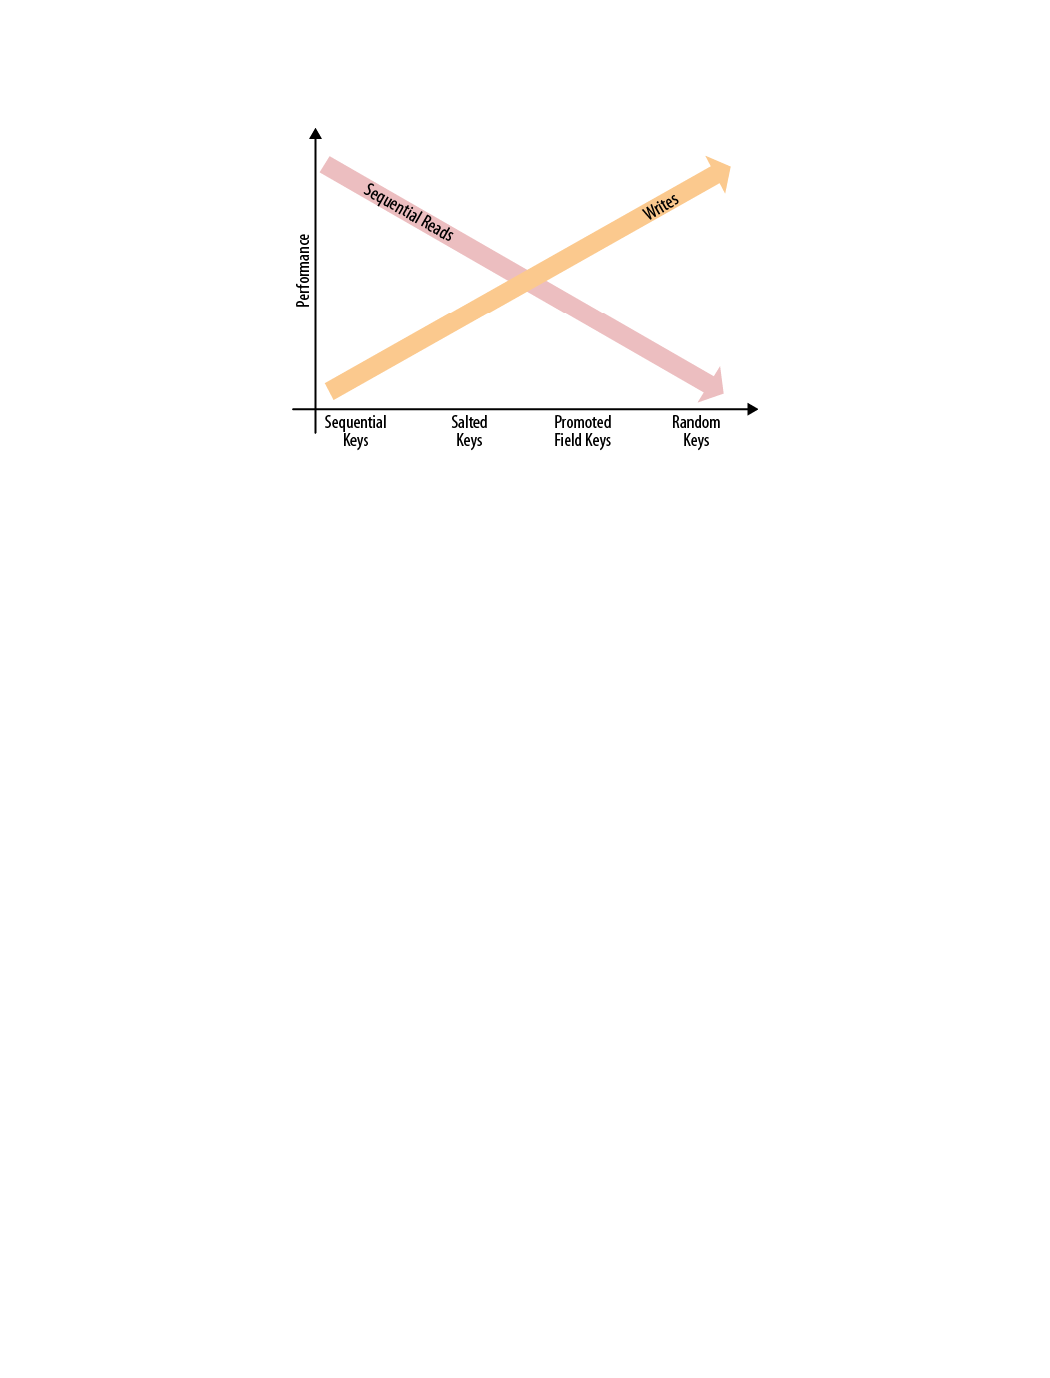
\includegraphics[scale=0.8]{./figures/time-series}
  \end{figure}

}

% %%%%%%%%%%%%%%%%%%%%%%%%%%%%%%%%%%%%%%%%%%%%%%%%%%%%%%%%%%
% \subsection{Time-Ordered Relations}
% %%%%%%%%%%%%%%%%%%%%%%%%%%%%%%%%%%%%%%%%%%%%%%%%%%%%%%%%%%
% \frame {\frametitle{}
% }


\subsection{MapReduce Integration}
%%%%%%%%%%%%%%%%%%%%%%%%%%%%%%%%%%%%%%%%%%%%%%%%%%%%%%%%%%
\begin{frame}
  \begin{beamerboxesrounded}{}
	\begin{center}

\vspace{20pt}

		MapReduce Integration

\vspace{20pt}

	\end{center}    
  \end{beamerboxesrounded}
\end{frame}


%%%%%%%%%%%%%%%%%%%%%%%%%%%%%%%%%%%%%%%%%%%%%%%%%%%%%%%%%%
\subsection{Recap}
%%%%%%%%%%%%%%%%%%%%%%%%%%%%%%%%%%%%%%%%%%%%%%%%%%%%%%%%%%
\frame {\frametitle{Introduction}
  \begin{itemize}
  \item \textbf{In the following we review the main classes involved in
      reading and writing data from/to an underlying data store}

    \vspace{20pt}

  \item \textbf{For MapReduce to work with HBase, some more practical issues
      have to be addressed}
    \begin{itemize}
    \item E.g.: creating an appropriate JAR file inclusive of all
      required libraries
    \end{itemize}

    \vspace{20pt}

  \item Refer to \cite{George2011}, Chapter 7 for an in-depth
    treatment of this subject
  \end{itemize}

}

\frame {\frametitle{Main classes involved in MapReduce}
  \begin{figure}[h]
    \centering
    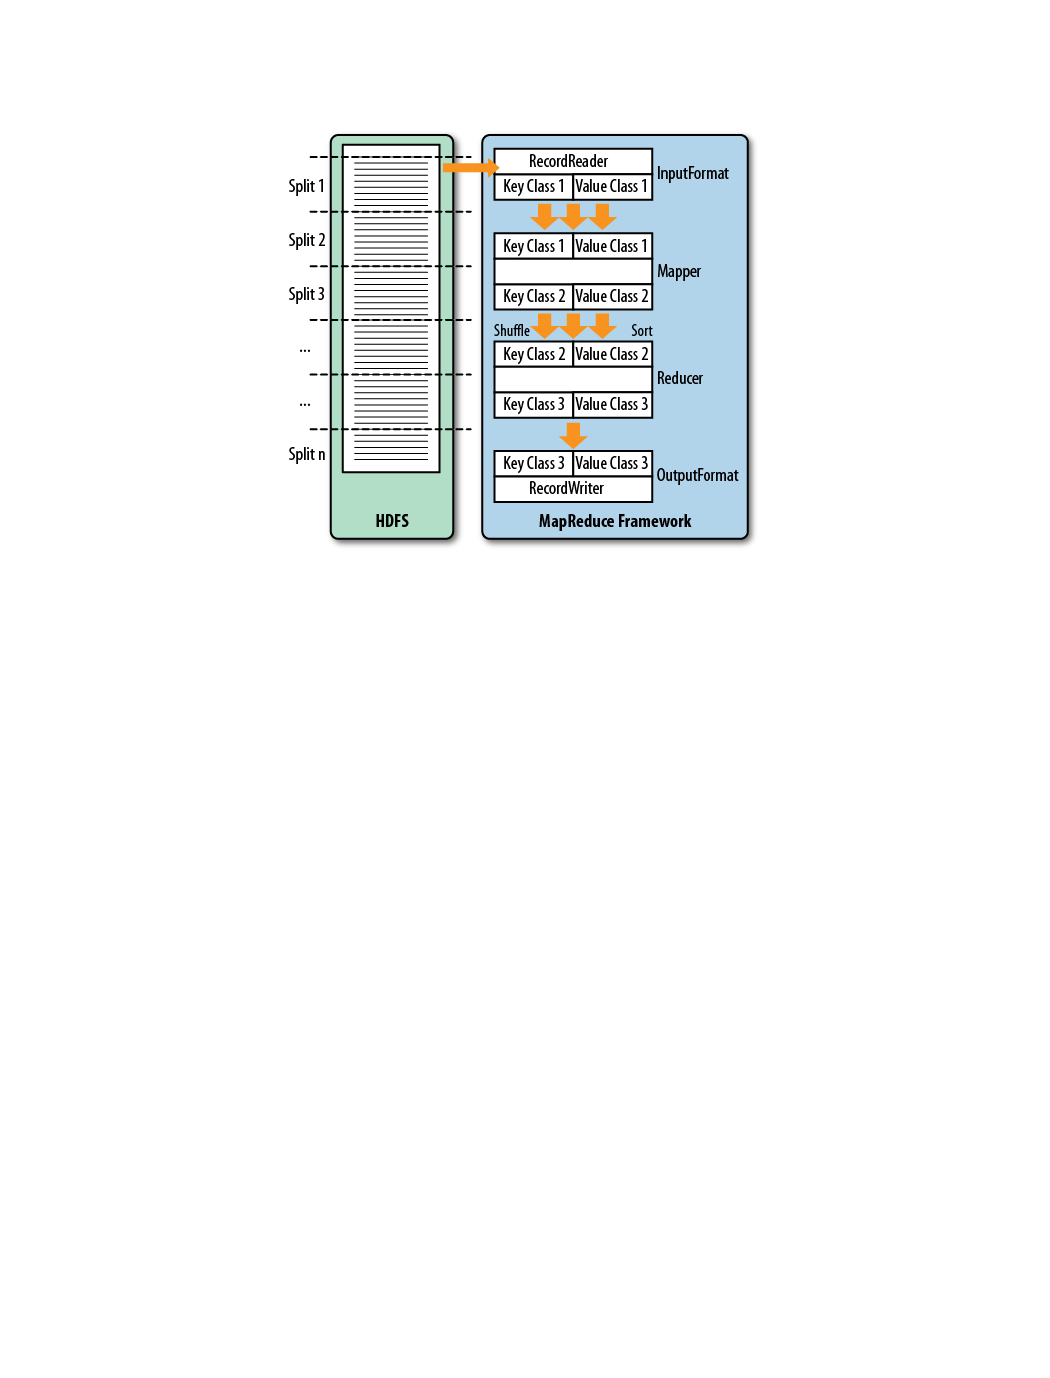
\includegraphics[scale=0.9]{./figures/mr-classes}
    \caption{Main MapReduce Classes}
  \end{figure}
}

\frame {\frametitle{Main classes involved in MapReduce}
  \begin{beamerboxesrounded}{}
    \texttt{InputFormat}
  \end{beamerboxesrounded}

  \begin{itemize}
  \item \textbf{It is responsible for two things}
    \begin{itemize}
    \item Splits input data
    \item Returns a \texttt{RecordReader} instance
      \begin{itemize}
      \item Defines a \textit{key} and a \textit{value} object
      \item Provides a \texttt{next()} method to iterate over input records
      \end{itemize}
    \end{itemize}
  \end{itemize}

  \begin{figure}[h]
    \centering
    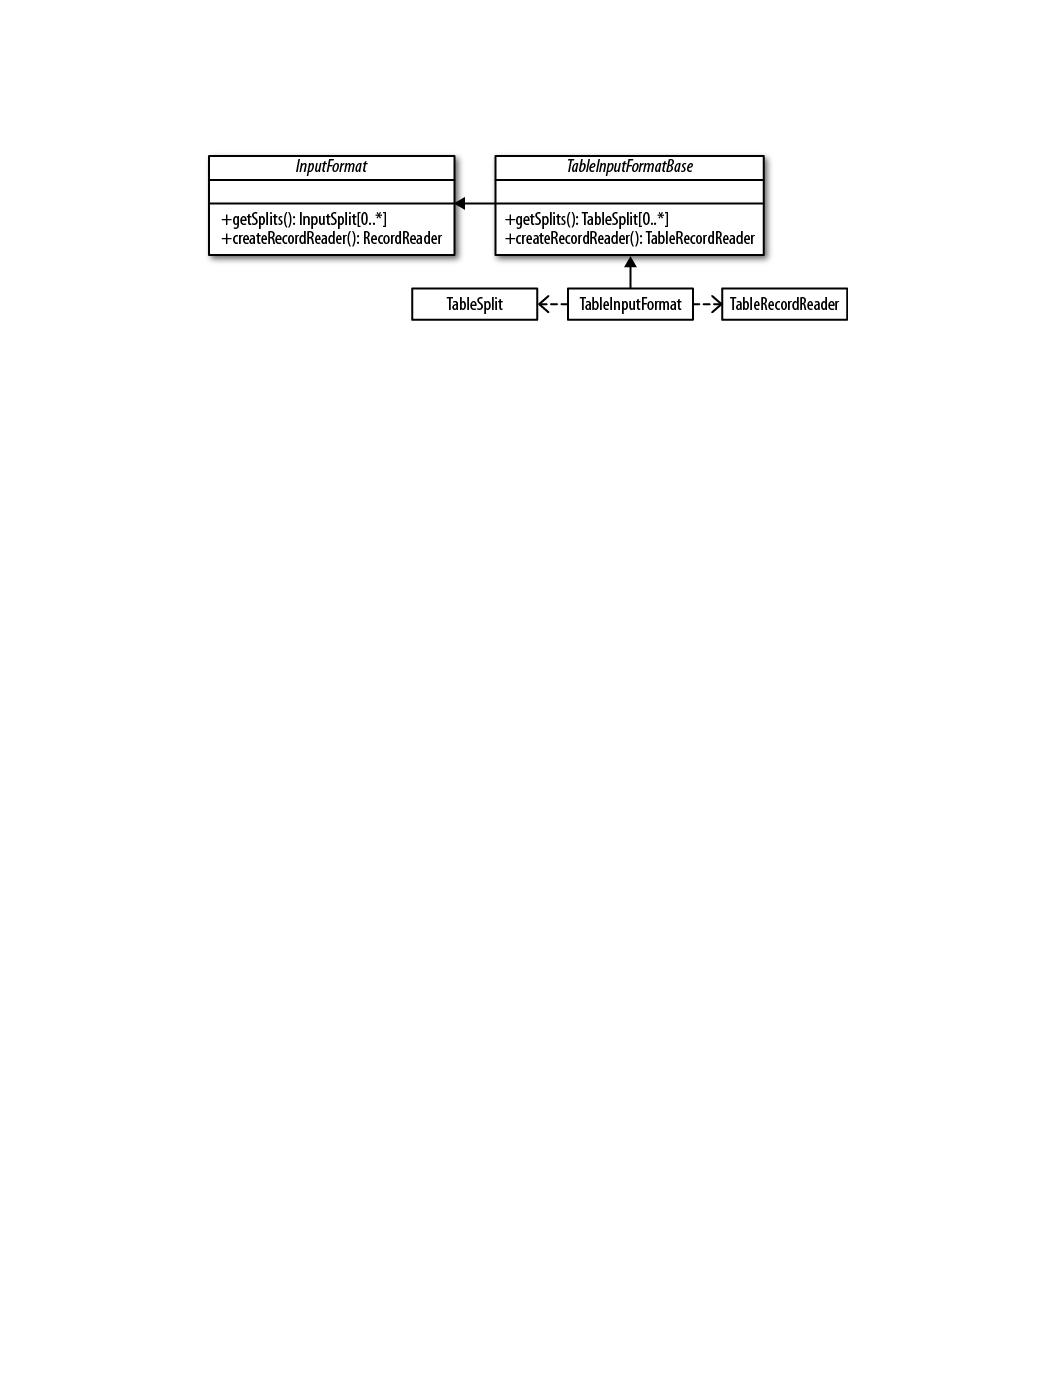
\includegraphics[scale=0.9]{./figures/input-format}
    \caption{InputFormat hierarchy}
    \label{fig:input-format}
  \end{figure}
}

\frame {\frametitle{Main classes involved in MapReduce}
  \begin{beamerboxesrounded}{}
    \texttt{InputFormat $\to$ TableInputFormatBase}
  \end{beamerboxesrounded}

  \begin{itemize}
  \item \textbf{Implement a full turnkey solution to scan an HBase
      table}
    \begin{itemize}
    \item Splits the table into proper blocks and hand them to the
      MapReduce process
    \end{itemize}

\vspace{20pt}

  \item \textbf{Must supply a \texttt{Scan} instance to interact with
      a table}
    \begin{itemize}
    \item Specify start and stop keys for the scan
    \item Add filters (optional)
    \item Specify the number of versions
    \end{itemize}
  \end{itemize}
}

\frame {\frametitle{Main classes involved in MapReduce}
  \begin{beamerboxesrounded}{}
    \texttt{Mapper}
  \end{beamerboxesrounded}

  \begin{itemize}
  \item \textbf{Each record read using the \texttt{RecordReader} is processed
    using the \texttt{map()} method}

  \vspace{20pt}

  \item \textbf{The \texttt{Mapper} reads specific types of input key/value
    pairs, but emit possibly another type}
  \end{itemize}

  \begin{figure}[h]
    \centering
    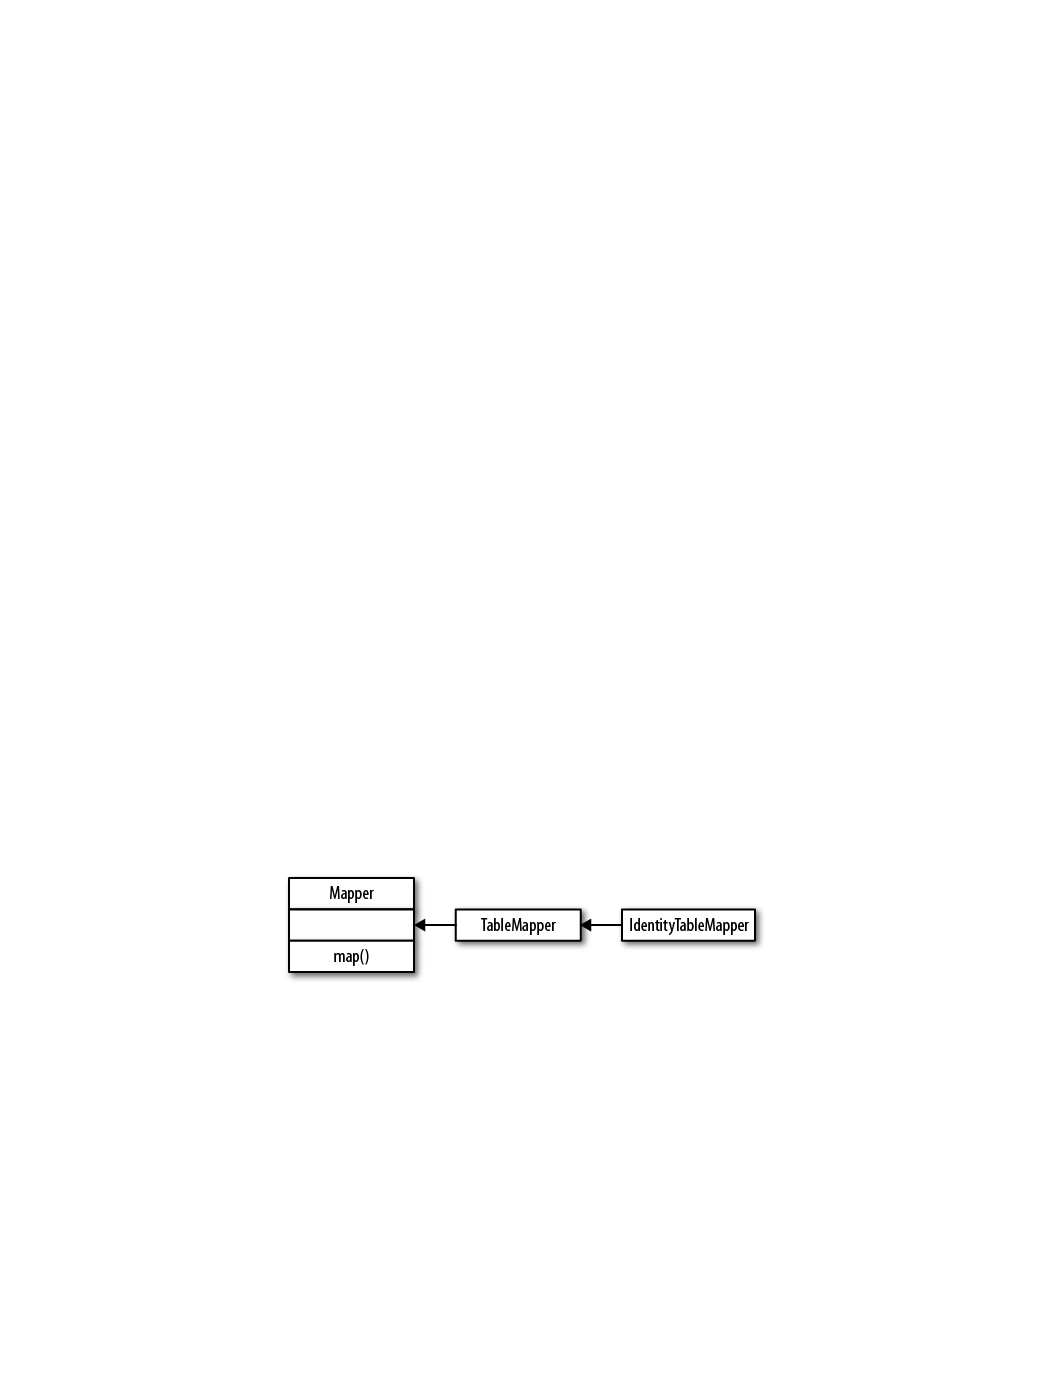
\includegraphics[scale=0.8]{./figures/mapper}
    \caption{The Mapper hierarchy}
    \label{fig:mapper}
  \end{figure}
}

\frame {\frametitle{Main classes involved in MapReduce}
  \begin{beamerboxesrounded}{}
    \texttt{Mapper $\to$ TableMapper}
  \end{beamerboxesrounded}

  \begin{itemize}
  \item \textbf{\texttt{TableMapper} class enforces:}
    \begin{itemize}
    \item The input key to the mapper to be an
      \texttt{ImmutableBytesWritable} type
    \item The input value to be a \texttt{Result} type
    \end{itemize}

    \vspace{20pt}

  \item \textbf{A handy implementation is the
      \texttt{IdentityTableMapper}}
    \begin{itemize}
    \item This is the equivalent of an identity mapper
    \end{itemize}
  \end{itemize}
}

\frame {\frametitle{Main classes involved in MapReduce}
  \begin{beamerboxesrounded}{}
    \texttt{OutputFormat}
  \end{beamerboxesrounded}

  \begin{itemize}
  \item \textbf{Used to persist data}
    \begin{itemize}
    \item Output written to files
    \item Output written to HBase tables
      \begin{itemize}
      \item This is done using a \texttt{TableRecordWriter}
      \end{itemize}
    \end{itemize}
  \end{itemize}

  \begin{figure}[h]
    \centering
    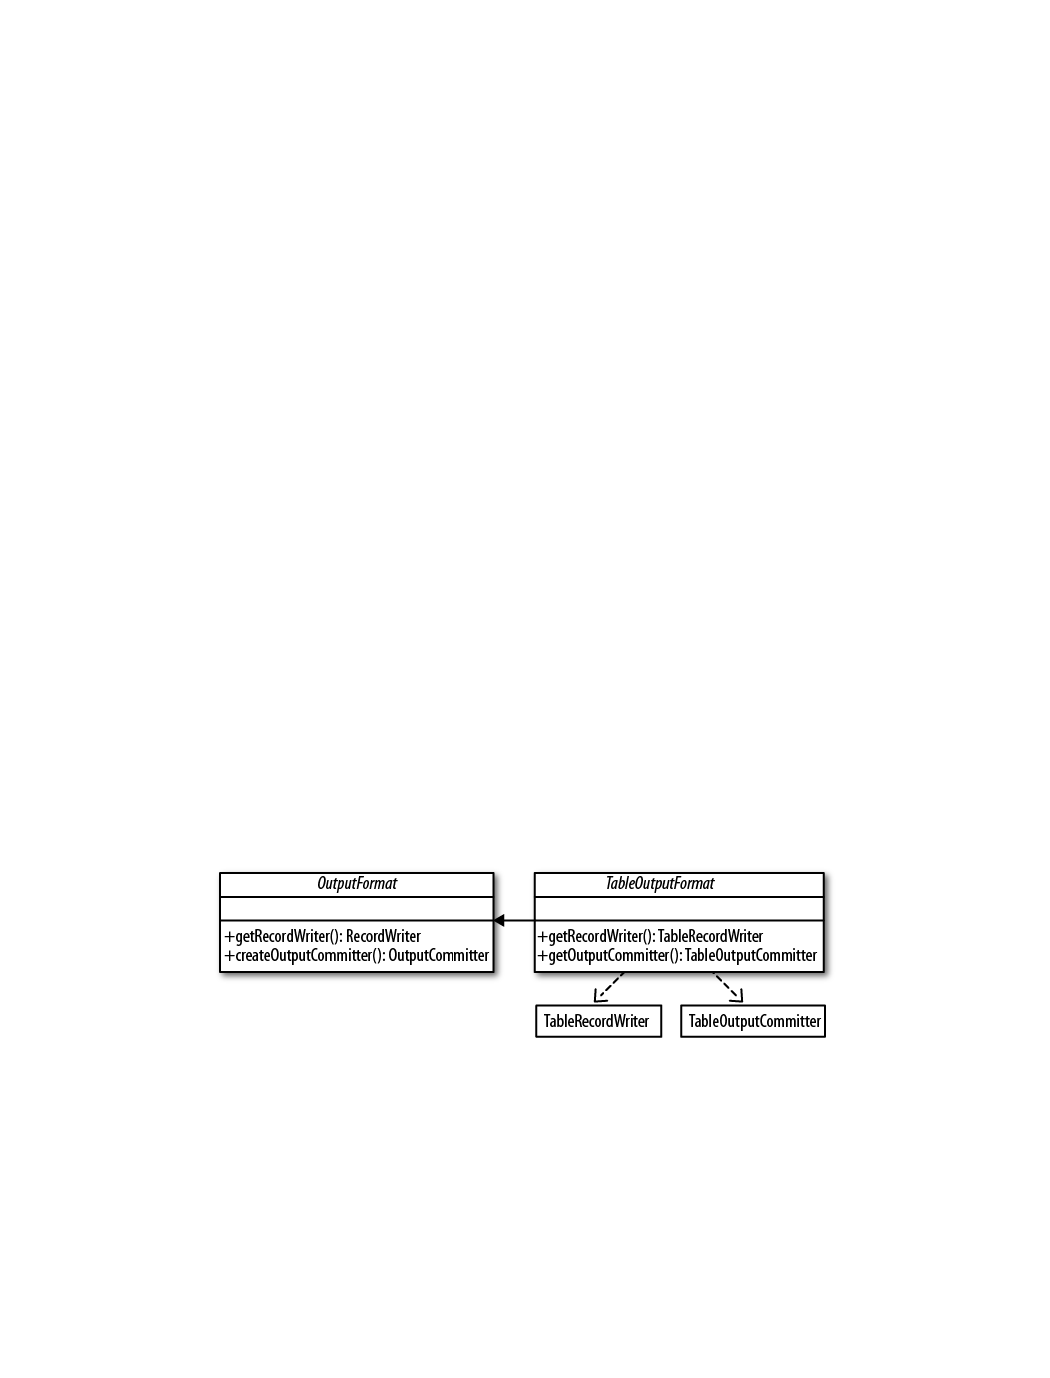
\includegraphics[scale=0.8]{./figures/outputformat}
    \caption{The OutputFormat hierarchy}
    \label{fig:outputformat}
  \end{figure}
}

\frame {\frametitle{Main classes involved in MapReduce}
  \begin{beamerboxesrounded}{}
    \texttt{OutputFormat $\to$ TableOutputFormat}
  \end{beamerboxesrounded}

  \begin{itemize}
  \item \textbf{This is the class that handles the key/valu pairs and writes
      them to their final destination}
    \begin{itemize}
    \item Single instance that takes the output record from each reducer subsequently
    \end{itemize}

    \vspace{20pt}

  \item \textbf{Details}
    \begin{itemize}
    \item Must specify the table name when the MR job is created
    \item Handles buffer flushing implicitly (\textit{autoflush} option is set to false)
    \end{itemize}
  \end{itemize}
}

\frame {\frametitle{MapReduce Locality}
  \begin{itemize}
  \item \textbf{How does the system make sure data is placed close to where it
      is needed?}
    \begin{itemize}
    \item This is done implicitly by MapReduce when using HDFS
    \item When MapReduce uses HBase things are a bit different
    \end{itemize}
    
    \vspace{20pt}
    
  \item \textbf{How HBase handles data locality}
    \begin{itemize}
    \item Shared vs. non-shared cluster
    \item HBase store its files on HDFS (\texttt{HFiles} and WAL)
    \item HBase servers are not restarted frequently and they perform
      compactions regularly
    \item[$\to$] HDFS is smart enough to ensure data locality
      \begin{itemize}
      \item There is a block placement policy that enforces local
        writes 
      \item The data node compares the server name of the writer with
        its own
      \item If they match, the block is written to the local filesystem
      \end{itemize}
    \item Just be careful about region movements during load balancing
      or server failures
    \end{itemize}

  \end{itemize}
}

\frame {\frametitle{Table Splits}
  \begin{itemize}
  \item \textbf{When running a MapReduce job that reads from an HBase table
      you use the \texttt{TableInputFormat}}
    \begin{itemize}
    \item Overrides \texttt{getSplits()} and \texttt{createRecordReader()}
    \end{itemize}

    \vspace{20pt}

  \item \textbf{Before a job is run, the framework calls getSplit() to
      determine how the data is to be separated into chunks}
    \begin{itemize}
    \item \texttt{TableInputFormat}, given the \texttt{Scan} instance
      you define, divide the table at region boundaries
    \item[$\to$] The number of input splits is equal to all regions
      between the start and stop keys
    \end{itemize}
  \end{itemize}
}


\frame {\frametitle{Table Splits}
  \begin{itemize}
  \item \textbf{When a job starts, the framework calls
      \texttt{createRecordReader()} for each input split}
    \begin{itemize}
    \item It iterates over the splits and create a new
      \texttt{TableRecordReader} with the current split
    \item Each \texttt{TableRecordReader} handles exactly one region,
      reading and mapping every row from the region's start and end keys
    \end{itemize}

    \vspace{20pt}

  \item \textbf{Data locality}
    \begin{itemize}
    \item Each split contains the server name hosting the region
    \item The framework checks the server name and if the
      \texttt{TaskTracker} is running on the same machine, it will run
      it on that server
    \item The \texttt{RegionServer} is colocated with the HDFS
      \texttt{DataNode}, hence data is read from the local filesystem
    \end{itemize}


    \vspace{20pt}

  \item \textbf{TIP: Turn off speculative execution!}


  \end{itemize}
}

%%%%%%%%%%%%%%%%%%%%%%%%%%%%%%%%%%%%%%%%%%%%%%%%%%%%%%%%%%
%%%%%%%%%%%%%%%%%%%%%%%%%%%%%%%%%%%%%%%%%%%%%%%%%%%%%%%%%%
\begin{frame}
 \begin{colorblock}{blue}{lightblue}{ }
  \begin{center}
    \Huge \textbf{\texttt{Cassandra}}
  \end{center}
  \end{colorblock}
\end{frame}
%%%%%%%%%%%%%%%%%%%%%%%%%%%%%%%%%%%%%%%%%%%%%%%%%%%%%%%%%%
%%%%%%%%%%%%%%%%%%%%%%%%%%%%%%%%%%%%%%%%%%%%%%%%%%%%%%%%%%
\section{Cassandra}

%%%%%%%%%%%%%%%%%%%%%%%%%%%%%%%%%%%%%%%%%%%%%%%%%%%%%%%%%%

% \section{References}
% \begin{frame}[allowframebreaks]{References}
% \bibliographystyle{plain} 
% \bibliography{references} 
% \end{frame}

\end{document}

%%%%%%%%%%%%%%%%%%%%%%%%%%%%%%%%%%%%%%%%%%%%%%%%%%%%%%%%%%
% PART SEPARATOR
%%%%%%%%%%%%%%%%%%%%%%%%%%%%%%%%%%%%%%%%%%%%%%%%%%%%%%%%%%

% \begin{frame}
%  \begin{colorblock}{blue}{lightblue}{ }
%   \begin{center}
%     \Huge \textbf{\texttt{Part One}}
%   \end{center}
%   \end{colorblock}
% \end{frame}
